\documentclass[12pt]{report}
\input{core/preambulo.tex}

%%%%%%%%%%%%%%%%%%%%%%%%%%%%%%%%%%%%%%%%%%%%%%%%%%%%%%%%%%
\newcommand{\nombreautor}{Vicente Antonio Muñoz L'Huillier}
\newcommand{\mes}{Julio}
\newcommand{\anio}{2022}
\newcommand{\titulo}{Inversión en capacidad de generación eléctrica cuando la atención del planificador es limitada}
\newcommand{\nombreprofuno}{Sebastián Cea Echenique}
\newcommand{\nombreprofdos}{Nombre Profe 2}
\newcommand{\nombreproftres}{Nombre Profesor Invitado}
\newcommand{\codigo}{ING-IN-001/11}

%%%%%%%%%%Aqui se escribe el resumen%%%%%%%%%%%%%%%%%%%%%
\newcommand{\resumen}{
Hacer resumen al terminar la tesis. Máximo 1 página
}

\newcommand{\agradecimientos}{
Muchas gracias a todos}

\newcommand{\dedicatoria}{\it
ok..
}
\renewcommand{\baselinestretch}{1.5}

%%%%%%%%%%%%%%%%%%%%%%%%%%%%%%%%%%%%%%%%%%%%%%%%%%%%%%%%%%

% Por favor coloque todas las definiciones de simbolos a continuacion
% y no en los archivos de capitulos. Esto evitara la  existencia de
% multiples definiciones para las mismas palabras.

\newcommand{\mydef}
	{\stackrel{\mathrm{def}}{=}}
\newcommand{\e}
	{\hbox{\large{e}}}
\newcommand{\mi}
	{\hbox{\large{i}}}
\newcommand{\RR}{\mathbb{R}}


%%%%%%%%%%%%%%%%%%%%%%%%%%%%%%%%%%%%%%%%%%%%%%%%%%%%%%%%%%

\begin{document}
\label{start}

% Genera las paginas de titulo, copyright, resumen,
% agradecimientos, dedicatoria, indices,...

% No es necesario modificar

% Paginas de titulo, derechos de autor y otras mas.

% Jaime Cisternas, julio 2004, agosto 2010

% declaracion especifica de pdfLaTeX
% permite incluir figuras con \includegraphics[...]{figurename}
\DeclareGraphicsExtensions{.jpg,.pdf,.mps,.png}

%%%%%%%%%%%%%%%%%%%%%%%%%%%%%%%%%%%%%%%%%%%%%%%%%%%%%%%%%%%%%%%%

  \pagenumbering{roman}
% \setcounter{page}{1}

% Escribe la pagina de titulo, incluyendo el autor y la facultad

  \thispagestyle{empty}
  \textsc{
  \vspace*{0cm}
  \begin{center}
    \Large
     Universidad de los Andes \\
     Facultad de Ingeniería y Ciencias Aplicadas\\
  \end{center}
     \vspace{1cm}
  \begin{center}
     \includegraphics[angle=0,height=5cm]{logos/Logo-UANDES.png}
  \end{center}
     \vspace{1cm}
  \begin{center}
     \Large
     \titulo
  \end{center}
  \vspace{0.5cm}
  \begin{center}
    \Large
    \nombreautor
  \end{center}
  \vspace{0.5 cm}
  \begin{center}
    Memoria para optar al título de \\
    Ingeniero Civil Industrial 
    Mención Gestión de Operaciones\\
    \vspace{1cm}
    Profesor Guía: \nombreprofuno \\
    \vspace{0.5cm}
    \codigo \\
    \vspace{0.5cm}
    Santiago, \mes\ de \anio
  \end{center}
  }

%%%%%%%%%%%%%%%%%%%%%%%%%%%%%%%%%%%%%%%%%%

% Escribe la segunda pagina de titulo para ser firmada por la comision

\cleardoublepage
\thispagestyle{empty}

\begin{center}

\vspace*{2cm}
\parbox{10cm}{
\noindent
Certifico que he leído esta memoria y que en mi opinión
su alcance y calidad son completamente adecuados como para ser considerada
una memoria conducente al título de Ingeniero.
\vspace{1cm}

\hfill
\begin{tabular}{c}
\hspace{8cm} \\
\hline
\nombreprofuno \\
(Profesor Guía)
\end{tabular}

\vspace*{1.5cm}

}

\end{center}

%%%%%%%%%%%%%%%%%%%%%%%%%%%%%%%%%%%%%%%%%%

% Espaciado entre lineas
  \onehalfspacing
  %\doublespacing

% Hace pagina de derechos de autor

  \cleardoublepage
  \thispagestyle{empty}
  %\vspace*{0in}
  \begin{center}
    \copyright\ \nombreautor\ \anio \\
    Todos los derechos reservados.
  \end{center}

%%%%%%%%%%%%%%%%%%%%%%%%%%%%%%%%%%%%%%%%%%%%%%%%%%%%%%%%%%%%%%%%%%%%%%

% Genera agradecimientos leyendo definicion de agradecimientos

  \cleardoublepage \addcontentsline{toc}{section}{Agradecimientos}
  \begin{center} \Large \textbf{Agradecimientos} \end{center}

Un primer agradecimiento se lo dedico a mi familia, por su constante apoyo tanto emocional como económico a lo largo de toda mi carrera universitaria. Agradezco la motivación y deseos de mejorar que me traspasaron durante todos estos años.
\vspace{2.5mm}

Un segundo agradecimiento es para el profesor Sebastián Cea que me ofreció la oportunidad de desarrollar la memoria con él y trabajar juntos en la mejora de su modelo. Su apoyo constante, reuniones continuas y el perfil personalizado con el cual me guió durante el último año, me permitió aprender y avanzar de forma ordenada en mi memoria. 
\vspace{2.5mm}

Un tercer agradecimiento se lo dedico a Felipe Feijoo por el taller que realizó sobre la resolución de problemas de equilibrio y su ayuda en el área computacional de este trabajo.
\vspace{2.5mm}

Finalmente, un agradecimiento a Orlando Contreras, tutor del Centro de Escritura, quien me apoyó con la redacción de este documento. Su ayuda tuvo un rol fundamental en el orden de mis ideas y el de este documento para realizar la mejor escritura posible.


% Genera resumen leyendo definicion de resumen


  \cleardoublepage
  \refstepcounter{dummy} \addcontentsline{toc}{section}{Resumen}
  \begin{center} \Large \textbf{Resumen} \end{center}
La presente memoria estudia la incorporación de atención racional en el modelo de \textit{cap and trade} de dos etapas creado por \citeB{amigo_two_2021}. Este modelo es una alternativa para fiscalizar las emisiones de dióxido de carbono de las empresas generadoras de electricidad, en que un subastador (también llamado planificador social) emite permisos que luego vende a las empresas generadoras y con los cuales ellas se limitan a contaminar.
\vspace{2.5mm}

La atención limitada guarda relación con la incapacidad de procesar toda la información disponible en la toma de decisiones. La inclusión de atención racional en el modelo se realiza porque la fijación del límite de emisiones implica un costo de adquirir o estimar esa información. La incorporación de este concepto es dificultoso en este modelo ya que este es un problema de optimización de capacidad con varios agentes y restricciones de equilibrio. Con el fin de resolver el problema, se deben transformar varios problemas en uno solo del tipo \textit{Mixed Complementarity Problem} (MCP, por sus siglas en inglés). La dificultad implícita es que el problema resultante es altamente no lineal.
\vspace{2.5mm}

En esta memoria se explica qué son los modelos de equilibrio, las condiciones de optimalidad, los MCP, se proporcionan ejemplos de cómo resolverlos en distintos lenguajes de programación y se replica el modelo original. Por último, se realiza la implementación de atención racional.
\vspace{2.5mm}

La implementación se realiza en el modelo del subastador. Se realizan dos versiones: \textit{Profit oriented}, en la cuál el subastador experimenta pérdidas según el rendimiento determinado y otra \emph{Welfare oriented} enfocada en el bienestar social (sobre la cual se realizaron dos formulaciones). Esta última optimiza el beneficio social en lugar de las utilidades económicas. 
\vspace{2.5mm}

Se resolvieron los nuevos modelos y se compararon con el original. Por un lado, los resultados del modelo \textit{Profit oriented} evidencian el impacto significativo del rendimiento en las variables óptimas del subastador. Este produjo, los precios de electricidad más bajos entre todos los modelos.
\vspace{2.5mm}

Por otro lado, el modelo Tasa Cuadrada (primera formulación \emph{Welfare oriented}) emite la menor cantidad de permisos para altos presupuestos de carbono. El Modelo con Precisión (segunda formulación \emph{Welfare oriented}) proporciona, junto al \textit{Profit oriented}, los precios de permisos de emisión más bajos para todos los presupuestos.
\vspace{2.5mm}

De acuerdo con lo anterior, se concluye que la propuesta aumenta el bienestar social y que existe potencial para perfeccionar ambas versiones y proponer una mejora al sistema.




% Genera dedicatoria

 % \cleardoublepage \vspace*{1.5in}
  %\begin{flushright} \dedicatoria %\end{flushright}

% Produce indice general, listas de figuras y de tablas

  \cleardoublepage
  \tableofcontents
  \cleardoublepage
  \listoffigures
  \cleardoublepage
  \listoftables
  \cleardoublepage

  \normalsize
  \pagenumbering{arabic}

%%%%%%%%%%%%%%%%%%%%%%%%%%%%%%%%%%%%%%%%%%%%%%%%%%%%%%%%%%%


%%%%%%%%%%%%%%%%Ingreso de capitulos%%%%%%%%%%%%%%%%%%%%%%

% cap1.tex

\chapter{Introducción}
\label{c1} % la etiqueta para referencias

En la actualidad, se reconoce a nivel mundial que el planeta está experimentando un cambio climático potencialmente perjudicial para la vida en él. También, múltiples estudios científicos y gran parte de la sociedad concuerdan en que muchas de las actividades del ser humano son un acelerador significativo de este cambio y el aumento de la temperatura. De acuerdo con diversos estudios, esto último apunta a que el aumento global de temperatura se debe al efecto invernadero, principalmente producido por $CO_2$. Este es un componente generado en un gran volumen por las actividades humanas tales como el transporte, la generación de energía, la ganadería, entre otros.
\vspace{2.5mm}

Esta situación ha generado un incentivo en las personas para encontrar soluciones y reducir el factor humano en el cambio climático. Con esto, se han producido importantes innovaciones y cambios en las industrias mencionadas y también se ha impulsado la creación de sistemas que permitan que estas transiciones sean sustentables y realistas en el largo plazo. 
\vspace{2.5mm}

Específicamente en Chile, la Estrategia climática de largo plazo de Chile (ECLP) presentada en el año 2021 por el Ministerio del Medio Ambiente concluye que el sector energético representó un 77\% de los gases de efecto invernadero producidos  en el año 2018 y, en ese sector, la generación de energía representa el mayor aporte con un 30\% del total de emisiones. Con el fin de disminuir este porcentaje, existen alternativas de generación más limpia que en la actualidad se emplean mayoritariamente. Sin embargo su implementación y producción es aún, en la mayoría de los casos, menos rentable, aunque la trayectoria de estas tecnologías muestra que, potencialmente, esto cambiará de forma positiva.
\vspace{2.5mm}

No obstante el trabajo realizado por \citeB{amigo_two_2021} demuestra que, con el sistema actual de penalización de emisiones que regula la industria generadora de electricidad, no es suficiente para lograr un cambio significativo y la reducción necesaria para lograr las metas prepuestas por Chile en el Acuerdo de París ni en el ECLP. Por lo tanto, los autores proponen un sistema de \emph{cap and trade} de dos etapas con mercado de compra y venta de permisos de contaminación. En este, las metas sí se logran cumplir y demuestra cómo es el efecto de este sistema con distintos presupuestos de contaminación. Sin embargo, este modelo propuesto presenta algunas limitaciones y posibilidades de mejora, que este trabajo busca aportar, específicamente sobre el problema del \emph{auctioneer} (subastador en inglés) de estos permisos de contaminación.


\section{Motivación}
Encontrar un modelo óptimo y eficiente para implementar en la industria de energía parece ser una tarea difícil. Muchos países tienen la intención de rebajar su aporte de contaminante global para alcanzar el acuerdo de París, pero una iniciativa no es suficiente, si no se respalda con continuo cambio y mejora. Cualquier tipo de modelo implementado a gran escala, como la fiscalización de la industria eléctrica, requiere de evaluación continua y estudio de implementaciones en otros países para encontrar cuál es la mejor solución al problema.
\vspace{2.5mm}

El ECLP dicta que Chile tiene como objetivo ser carbono neutral\footnote{Carbono neutral no significan 0 toneladas de dióxido de carbono emitidas, sino que las emisiones sean iguales a las absorciones por agentes como el sector forestal.} como fecha límite para el año 2050. A la fecha, el país tiene como estrategia para disminuir las emisiones de la industria eléctrica aplicar un ``impuesto verde'' descrito en la ley 20.780 promulgada en el año 2014. Diversos estudios (mencionados en el marco teórico de este trabajo) argumentan que esto no es suficiente y su aplicabilidad no es sustentable y no incentiva el cambio a energías renovables. En efecto, los autores \citeB{amigo_two_2021} demuestran y concluyen que, en primer lugar, el objetivo de carbono neutralidad es lograble y, en segundo lugar, que el \emph{National Determined Contribution}  (NDC por sus siglas en inglés)\footnote{National Determined Contribution: Aporte del país en la propuesta del acuerdo de París}  propuesto para el acuerdo de París\footnote{En el acuerdo de París se estableció como objetivo no superar un aumento global de temperatura de 2 °C para finales de este siglo.}, que consiste en que, para el año 2030, el nivel de $CO_2 e$ (dióxido de carbono emitido) no supere los 131 $MtCO_2 e$ en Chile, es una meta fácil de lograr y, por lo tanto, ineficiente. Ellos proponen la implementación de una versión de su modelo de \emph{cap and trade}, con la cuál se pueden alcanzar objetivos mucho más ambiciosos en la reducción de emisiones y sobre el cambio a una generación de energía con fuentes sustentables.
\vspace{2.5mm}

Entonces, el propósito de este trabajo es aportar en la investigación, testeo y complementación del modelo para así demostrar que existe un sistema mejor al actualmente utilizado. La finalidad es combatir el problema del cambio climático y que las empresas generadoras puedan seguir funcionando, que sean rentables y que aporten en el desarrollo de las nuevas tecnologías no convencionales.


\section{Objetivos}
\subsection{Objetivo general}
El objetivo general de este trabajo es mejorar la racionalidad del planificador social por medio de la incorporación de nuevos factores en su función objetivo. Por ejemplo, mediante restricciones que influencien el valor óptimo de permisos que este debe emitir con la finalidad de introducir incentivos para que este se convierta en un actor económico que busca cumplir criterios medioambientales asumiendo costos de investigación. En otras palabras, se busca formular penalizaciones en las utilidades del subastador que le incentiven producir una mejor emisión de permisos.

\subsection{Objetivos específicos}
Los objetivos específicos necesarios para lograr el objetivo general son:

\begin{enumerate}
\item Identificar modelos de equilibrio y modelos de equilibrio en capacidad.
\item Identificar métodos de resolución de MCP.
\item Programar problemas MCP en GAMS.
\item Replicar modelo original de Amigo.
\item Implementar mejora en problema del subastador o \emph{auctioneer}.
\item Simular el nuevo modelo y analizar resultados.
\end{enumerate}


\section{Alcances}
Los alcances de este trabajo se circunscriben a resultados teóricos encontrados implementando el nuevo modelo en un \emph{solver}. Entonces, el alcance está definido según lo realizado para encontrar esos resultados en el \emph{solver}, que incluye la replicación del modelo original, la mejora del modelo y luego encontrar sus soluciones para finalmente evaluar estas soluciones.
\vspace{2.5mm}

Primero, se lleva a cabo la replicación del modelo original de Amigo. Para esto es necesario entender el modelo propuesto y saber como resolverlo. Uno de los métodos más eficientes para resolver un problema de esta complejidad y encontrar soluciones para sus variables es resolviendo el problema como un MCP. Pero primero es necesario definir el modelo acorde a lo que un MCP solicita para su realización. Por lo que fue necesario aplicar las condiciones de KKT que como resultado otorgan las condiciones necesarias para resolver el problema como MCP. Por lo que el alcance en esta etapa del proyecto es encontrar las mismas soluciones que el \textit{paper}.
\vspace{2.5mm}

Segundo, la mejora del problema del subastador representa un alcance de entregar una descripción más acertada de como un subastador en un modelo de \textit{cap and trade} debería funcionar y como sus decisiones pueden ser representadas en un problema de optimización.
\vspace{2.5mm}

REVISAR ESTO ANTES SI SERÁ FINALMENTE ASÍ Finalmente, programar el nuevo modelo y encontrar sus soluciones tienen como objetivo lograr que el modelo mejore o sea más certero a si este sistema se implementa en la realidad. No se espera necesariamente encontrar mejores resultados respecto a que se logre acotar aún más las emisiones de carbono o eliminar eliminar la producción con carbón antes de lo encontrado en el modelo original. Entonces el modelo nuevo tiene como objetivo mejorar la interpretación y predicción teórica de lo que se podría realizar en la realidad pero queda fuera de alcance la implementación real del sistema.  

\section{Metodología}
Este trabajo se divide en las siguientes etapas mencionadas anteriormente, pero se detallan con profundidad de la siguiente forma:

\begin{enumerate}
\item Identificar modelos de equilibrio y modelos de equilibrio en capacidad: con bibliografía recomendad por el profesor guía y bibliografía metódicamente filtrada según estándares descritos según publicador y otras características, se lleva a cabo un estudio de los modelos de equilibrio.
\item Identificar métodos de resolución de MCP : para resolver los problemas de equilibrio es posible transformarlos en MCP al aplicar las condiciones de KKT. Se estudió principalmente de un curso realizado por Felipe Feijoo en el verano del año 2022 llamado "Computo de modelos de equilibrio", organizado por Sebastián Cea y la facultad de ingeniería de la Universidad de los Andes.   
\item Programar problemas MCP: es necesario aprender sobre distintos solvers de MCP y softwares que lo soporten. Primero, se realizan ensayos de programación con problemas de similar naturaleza al de Amigo en \citeB{d__aertrycke_risk_2017}. Finalmente, se busca profundizar con el curso de Felipe Feijoo sobre MCP. 
\item Replicar modelo original de Amigo: se desarrollan las condiciones de kkt y formulación de MCP para resolver el modelo original. Luego, se ejecuta el código original con los parámetros utilizados en el \textit{paper} para visualizar resultados y entender el funcionamiento.
\item Implementar mejora en problema del subastador o \textit{autioneer}: se encuentra una reestructuración del problema del subastador por medio de estudio sobre costos asociados al incentivo de mejora en \textit{performance}.
\item Evaluar nuevo modelo en \textit{solver} y analizar resultados: se evalúa el nuevo modelo al ejecutarlo en un \textit{solver} y se analizan las variables óptimas encontradas.
\end{enumerate}


\section{Estructura del documento}






% cap2.tex

\chapter{Marco Teórico}
\label{c2} 


\section{\textit{Cap and Trade} y otros sistemas actuales}\label{c22}
%Agregar desde segundo párrafo de la Revision bibliográfica del hito 1

En el contexto de la generación de energía, el medio ambiente es directamente afectado por la tecnologías utilizadas. Con el fin de generar energía, se necesita de la combustión de un material, el aprovechamiento mecánico de una energía natural externa u otra fuente como energía nuclear. Estos sistemas provocan, en distintos niveles y formas, efectos en el medio ambiente. Particularmente, las termoeléctricas son consideradas como las que más emisiones de dióxido de carbono producen.
\vspace{2.5mm}

La última importante mención por parte del Gobierno de Chile, sobre su plan para combatir esta situación, es la propuesta climática a largo plazo que el Ministerio del Medio Ambiente de Chile presentó en la COP26 el mes de octubre de 2021 (\citeB{gobierno_de_chile_estrategia_2021}). En ella, se proponen medidas drásticas para combatir las emisiones por medio de una propuesta específica en la Sección de generación de energía. En ella, se presenta un presupuesto límite de emisión de carbono para los generadores de energía. Sin  embargo, en contraste, no se incluye un mecanismo o plan específico de cómo las empresas generadoras lograrán esto y de qué forma se llevará a cabo la supervisión de esta meta.
\vspace{2.5mm}

Desde que se identificó al efecto invernadero como un problema, varios países han comenzado a intervenir, directa o indirectamente, en las industrias que más aportan al efecto. 
\vspace{2.5mm}

Por un lado, el impuesto al carbono o impuesto a emisiones de $CO_2$ consiste en un costo adicional para la generación de electricidad con energías no renovables. El impuesto es cobrado por cada tonelada emitida de este compuesto. \citeB{asen_carbon_2021} menciona que Finlandia, en 1990, fue el primer país en implementarlo y desde ese momento 18 otros países del continente y muchos otros en el planeta lo fueron aplicando a distintos valores por tonelada emitida.
\vspace{2.5mm}

Por otro lado, existen los modelos de \textit{cap and trade}, concepto creado por Thomas Crocker. Según \citeB{hanemann_cap-and-trade_2010} este consiste en que un ente regulador determina capacidades máximas de contaminación por emisiones a las empresas de la industria eléctrica. Estos emisores son regulados y se les asignan permisos con determinados márgenes, por lo tanto, si superan la capacidad permitida, deben pagar penalizaciones.
\vspace{2.5mm}

En un contexto en el cual se busca cumplir con promesas por país para lograr el acuerdo de París (no aumentar la temperatura global en más de 2°C para fines del siglo), un modelo de \textit{cap and trade} es el que se presenta como una mejor opción. Esto se debe a que permite establecer, inicialmente, capacidades límites por industria o por país. Entonces, la regulación de un máximo de contaminación es más factible con un modelo que limite el contaminante de cada agente contaminador. Sin embargo, el problema radica en que cada tipo de \textit{cap and trade} implementado puede afectar en distintas formas la industria, las empresas involucradas y la demanda energética. Por un lado, se puede lograr minimizar emisiones gracias a la reducción en la generación y, por otro lado, se puede lograr aumentar la cantidad de empresas generadoras con energías renovables.
\vspace{2.5mm}

\citeB{chen_renewable_2021} prueban que aplicar un mecanismo de \textit{cap and trade} es mucho más efectivo en reducir las emisiones de carbono y en incentivar la inversión en energías renovables en comparación con no implementar ningún mecanismo de \textit{cap and trade}. Los autores estudian 3 escenarios aplicados a una empresa monopólica. Los escenarios son los siguientes: sin mecanismo de cap-and-trade (NM), con \textit{cap and trade} de regla Grandfathering (GM)\footnote{Mecanismo en el cuál una cuota total de carbono emitido  se determina para cada empresa según sus emisiones pasadas. \cite{chen_renewable_2021}} y mecanismo de \textit{cap and trade} con regla Benchmarking (BM).\footnote{El gobierno determina una cuota por unidad de carbono emitido.\cite{chen_renewable_2021}} 
\vspace{2.5mm}

El estudio concluye que al implementar mecanismos siempre existirá una mejora en el área de inversión en energías no convencionales o en la reducción en emisiones de carbono. No obstante también concluyen que un aumento en la inversión en energías renovables no reduce necesariamente las emisiones de carbono totales, debido a que esta inversión puede ser resultado o respuesta únicamente del aumento en generación y no un reemplazo de generación con un nuevo tipo de origen. Entonces, además demuestran que la implementación de BM incentiva más este tipo de inversión y, por el contrario con GM se produce menos emisiones de carbono. De esto, es importante destacar que el tipo de mecanismo de \textit{cap and trade} afecta en gran medida el resultado, entonces se debe construir un modelo que logre las promesas de contaminación propuestas y no implementar cualquier mecanismo. 
\vspace{2.5mm}

\citeB{wang_impact_2021} se focalizan en el efecto que las implementaciones de los mecanismos \textit{Benchmarking} y \textit{Grandfathering} tienen en las cadenas de suministro de las empresas. Se evalúan cómo los modelos de financiamiento Bank Credit Financing (BCF)\footnote{El banco otorga un crédito con la necesidad de que se aplique a bajar emisiones de la empresa prestataria.\cite{wang_impact_2021}} y Trade Credit Financing (TCF)\footnote{Crédito que permite atrasar el pago del manufacturero al proveedor.\cite{wang_impact_2021}}, en conjunto con BM y GM, afectan las cadenas de suministro de las empresas y de que forma estas se comportan. Se observa el comportamiento de un productor y su proveedor. Finalmente, se concluye que sin importar el mecanismo de \textit{cap and trade}, los productores o fabricantes siempre prefieren BCF, mientras que los proveedores se inclinan por TCF. Además, el tipo de mecanismo que sea conveniente para el productor dependerá principalmente de sus emisiones históricas.
\vspace{2.5mm}

En estos estudios, se reconoce la importancia de la implementación del tipo de modelo y de cómo el presupuesto de carbono total puede afectar al mercado. A pesar de esto, el mismo creador del modelo de \textit{cap and trade} mencionó, en el año 2009, ``Soy escéptico de que un modelo de cap-and-trade sea la forma más eficaz de regular el carbono'',\footnote{{\scriptsize \url{https://www.businessinsider.com/inventor-of-cap-and-trade-says-a-carbon-tax-is-better-2009-8}}} debido a que él concluía que era difícil predecir cómo este modelo afectaría al mercado de generación en el futuro, además, si no se tiene un ente regulador, que fiscalice las emisiones continuamente y establezca las capacidades de forma apropiada, un modelo únicamente con impuesto a la emisión parece ser más eficaz. Entonces, un modelo que se pueda regular solo, en el cual exista incentivo en la disminución de emisión, en el que las empresas generadoras tengan más de una oportunidad para cambiar sus inversiones en capacidad y permisos y que este cambio signifique un beneficio para las empresas, sería un camino apropiado para un modelo de \textit{cap and trade} efectivo. Los autores \citeB{amigo_two_2021} proponen un sistema con estas características.


\section{Problemas de equilibrio en capacidad} \label{c21}

Con el fin de interpretar la toma de decisiones de los agentes en cualquier sistema, es necesario modelar los mecanismos en los cuales están involucrados los diferentes actores. Los modelos de optimización bien diseñados orientan la toma de decisiones en base a variables que pueden describir la estrategia de un agente. Estas variables son interpretación de qué decisiones deben tomar los agentes involucrados mientras estos tengan el poder de cambiarlos. 
\vspace{2.5mm}

Un modelo bien estructurado, con restricciones basadas en la teoría económica, puede, por una parte, significar un cambio operacional y táctico para una empresa o actor que busca optimizar algún problema. Por otra parte, un modelo puede mostrar el comportamiento esperado de un mercado.
\vspace{2.5mm}

Los modelos de equilibrio son aquellos que representan un problema donde los tomadores de decisión (representados por conjuntos de variables y funciones objetivos en el modelo) cumplen con una optimalidad individual y restricciones de equilibrio asociadas a sus decisiones que relacionan las acciones óptimas de todos los agentes involucrados.
\vspace{2.5mm}

Estos modelos, por ejemplo, representan las estrategias de varios agentes involucrados para el abastecimiento de una demanda de mercado. 
\vspace{2.5mm}

Esta memoria se focaliza en los modelos de equilibrio en capacidad, relacionados con el mercado de generación eléctrica. En estos, por una parte, presentan un equilibrio entre la demanda de energía de los consumidores y la oferta de los productores y, por otra parte, un equilibrio entre la capacidad instalada de los productores y los permisos para emitir contaminantes. Este problema se formula como la minimización anual de inversión en las plantas generadoras de energía.
\vspace{2.5mm}

Los modelos de equilibrio en capacidad han sido estudiados por \citeB{ehrenmann_generation_2011}, \citeB{d__aertrycke_risk_2017}, \citeB{gabriel_complementarity_2012}, \citeB{ralph_risk_2015}, entre otros.
\vspace{2.5mm}

A continuación, en base al trabajo de \citeB{d__aertrycke_risk_2017}, se explica un problema de equilibrio en capacidad con riesgo asociado de dos etapas y uno de riesgo neutral.

\subsection{Problema de equilibrio en capacidad con riesgo asociado (\textit{risky design equilibrium problem}) y modelos de dos etapas}

En este tipo de problemas, existe una variable o vector de variables de diseño denotada como  $x \in \mathbb{R}^{n}$, la cual describe la inversión en activos riesgosos tales como plantas de producción de energía que llevan consigo poderes de producción determinados y proporcionales al grado de inversión en mercados con incertidumbre de demanda.
\vspace{2.5mm}

Es importante entender que estos son problemas de optimización estocásticos. Es decir, existe aleatoriedad respecto a los parámetros de entrada. En este caso, la aleatoriedad se ve reflejada en los escenarios estocásticos posibles con $w \in \Omega:=\{1,...,K\}$. Entonces, por ejemplo, existen costos $C^{w}$ que corresponden a cada escenario $w$. 
\vspace{2.5mm}

La probabilidad de ocurrencia de cada escenario depende de una distribución de probabilidad $\Theta$, la cuál debe ser definida en el problema estudiado y una de sus aplicaciones es con la notación de valor esperado $E_{\Theta}[Z]$. Esta corresponde a la suma ponderada con una probabilidad de ocurrencia para una realización particular $z_{w}$ de la variable aleatoria $Z$ . En otras palabras, $E_{\Theta}[Z]$ es una suma ponderada de los valores de una variable en todos los escenarios multiplicados por la probabilidad de ocurrencia de cada escenario. En el Anexo \ref{ej:sumapond} se presenta un ejemplo de lo anterior.
\vspace{2.5mm}

Generalmente, estos modelos, tienen dos etapas de decisión $s\in\{0,1\}$ para los agentes diseñados en el problema. En la primera etapa $s=0$, el productor (monopolio) o grupo de productores (mercado competitivo) decide su inversión en capacidad $x$. Luego, en la segunda etapa $s=1$, se decide la producción $Y$ (si existe más de un escenario de ocurrencia, estos presentan distintas demandas o costos). Es decir, la variable de producción también puede depender del escenario $w$, teniendo $Y_{w}$ para cada uno).
\vspace{2.5mm}

 \citeB{d__aertrycke_risk_2017}, identifican estos problemas como aquellos en los que existe una función $f$ convexa y continua, $g$ convexa y continua en los que para cada $x$:

\begin{align}
\min f(x,y)\quad\text{sujeta a}\quad g(x,y)\leq 0
\end{align}


Este problema de optimización busca minimizar los costos asociados al problema y $g(x,y)$ puede ser una o un grupo de restricciones tecnológicas o de equilibrio del sistema.\footnote{Ver página 11 de \citeB{d__aertrycke_risk_2017}.} 
\vspace{2.5mm}

Con el fin de contrarrestar los costos asociados a escenarios con incertidumbre, por ejemplo, sub o sobre inversión, según cada escenario, cada agente $i$ se dota de una medida de riesgo $r_{i}$ que mide el costo de la incertidumbre respecto de una variable incierta (variable aleatoria o estocástica). Para mitigar ese costo por riesgo, el agente puede decidir qué productos financieros $W_i\in\mathbb{R}^K$ elegir para compensar el riesgo de incertidumbre en cada escenario. Estos productos tienen un precio asociado $P^{r}[W_i]$. Este precio es determinado por la condición de que todos los productos financieros deben balancearse y, suponiendo que $N>0$ agentes componen el mercado, lograr que:

\begin{eqnarray}
\sum_{i=1}^{N}W_{i} &=& 0\label{eq:fin-eq}    
\end{eqnarray}

En otras palabras, si un agente necesita un contrato o producto financiero que asegure un determinado valor en el escenario $w$, la condición de equilibrio o balance (ecuación \ref{eq:fin-eq}) anterior asegura que existe otro agente dispuesto a entregar (o prestar) ese valor. Esa entrega o préstamo tiene un valor determinado endógenamente por $P^r$.\vspace{2.5mm}

En cada una de las dos etapas de este sistema, existen importantes consideraciones.
\vspace{2.5mm}

En la primera etapa, la empresa generadora toma una decisión de inversión en capacidad $x$ que acotará la máxima producción. 
\vspace{2.5mm}

En la segunda etapa, se conoce la demanda del periodo y la empresa generadora minimiza sus costos. La producción es $Y_{w}$ para el escenario $w$ y se vende la energía a un precio $P_{w}\geq 0$ y costo $C_{w}(Y_{w})$. En cada escenario $w$, la empresa buscará maximizar las utilidades o minimizar los costos de operación y, al mismo tiempo, el demandante buscará maximizar sus utilidades de demanda $Q_{w}$ al comprar la energía al precio $P_{w}$.

\subsection{Tratamiento del riesgo}

La forma en cómo se valora el riesgo usualmente se ha clasificado entre aversos, neutrales y amantes. Dicha tipología tiene directa relación con la curvatura de la función objetivo que evalúa un valor incierto. La aversión al riesgo se representa mediante la concavidad, la neutralidad con funciones lineales como un valor esperado y el gusto por riesgo con convexidad. En lo que sigue nos centraremos en el caso estándar de riesgo neutralidad como supuesto simplificador.

Este es el caso en el que todos los agentes involucrados en el problema conocen sus costos estocásticos del problema con la probabilidad $\Theta$ anteriormente explicada de cada escenario $w$. Esto significa que aquellos costos asociados a la producción respetan esta probabilidad, sin embargo los costos de inversión en capacidad no son estocásticos, por lo tanto, no son afectados directamente por esta. En el caso neutral al riesgo, existe solamente el riesgo en inversión de capacidad, pero no un riesgo de compra de activos financieros ya que los agentes, en este caso, son neutrales al riesgo de intercambio o compra de activos financieros. 
\vspace{2.5mm}

Como se mencionó anteriormente, este estudio explora la aplicación de estos modelos en el mercado de empresas generadoras de electricidad, en que existen dos tipos de agentes: empresas generadoras únicamente de electricidad y demandantes de la energía producida. Este es un caso que puede ser tomado como de mercado competitivo, en el que las empresas no actúan estratégicamente para influenciar los precios. 
\vspace{2.5mm}

Bajo estas circunstancias, se tiene que este es un problema competitivo de equilibrio en capacidad riesgo neutral si es que existe un grupo de variables, $x_{1}$ para la inversión en capacidad del primer generador, $Y$ para la cantidad ofertada de electricidad para cada escenario $\omega$), $x_{2}$ para la inversión en capacidad del segundo generador, y $Q$ para la demanda energética. El problema debe resolver lo siguiente: 

\begin{align}
 \text{min } I_{1}(x_{1})+ I_{2}(x_{2})+E_{\Theta}[C_{w}(Y_{w}-U_{w}(Q_{w})] \label{foejemplomaere}
\end{align}

sujeto a

\begin{align}
 x_{1} \in X_{1} ,x_{2} \in X_{2}\label{res1ejemplomaere}\\
A_{1w}x_{1}+B_{1w}Y_{w}+b_{1w} \le 0 \label{res2ejemplomaere}\\
A_{2w}x_{2}+B_{2w}Y_{w}+b_{2w} \le 0 \label{res3ejemplomaere}\\
Q_{w}\le e^{\tau}Y_{w}\text{  }\text{ para todo w}\label{res4ejemplomaere}
\end{align}

Modelo en el cuál, la función objetivo \ref{foejemplomaere} minimiza el negativo de utilidad. La restricción \ref{res1ejemplomaere} acota la elección de estrategia de inversión para cada agente según su \textit{set} de estrategias $X_i$. Las restricciones \ref{res2ejemplomaere} y \ref{res3ejemplomaere} acotan los recursos de cada agente según su capacidad de inversión y oferta. La última restricción \ref{res4ejemplomaere} solicita que la demanda se debe abastecer completamente.



\section{MCP y Programación modelos de equilibrio}

\subsection{Resolución Problemas de equilibrio mediante MCP}\label{descripcionkkt}

La mayoría de los estudios sobre modelos de equilibrio, mencionados anteriormente, explican que la mejor forma de resolver los problemas de este tipo, en especial aquellos con gran cantidad de variables o aquellos no lineales, es transformarlos en problemas de complementaridad mixta o \textit{Mixed Complementarity Problems} (MCP por sus siglas en inglés, ver objetivo específico b) en el capítulo introductorio).
\vspace{2.5mm}

\citeB{gabriel_complementarity_2012} explican que para realizar esto, es necesario estructurar el problema de equilibrio de la siguiente forma:

\begin{align}
    \min_{x} & \quad f(x) \label{foej1}\\ 
    \textrm{s.a.} \nonumber\\
    g_{i}(x) \leq 0 ,\quad & i=1,2,...,n  &(\eta_{i}) \label{resej1} 
\end{align}

Con $f(x)$ función objetivo,  $g_{i}(x):\mathbb{R}^n \rightarrow \mathbb{R}$ restricciones y $\eta_i$ los multiplicadores de Lagrange asociados. 
\vspace{2.5mm}

Puede suceder que las restricciones son con sentido inverso y para eso solo basta con multiplicar la restricción \ref{resej1} por $-1$ y así obtener el sistema de ecuaciones deseado. Si la función objetivo \ref{foej1} es una maximización, basta con multiplicarle $-1$ a la función para convertirla en minimización.
\vspace{2.5mm}

Luego, se debe calcular el Lagrangeano de este problema con las variables duales de cada restricción ($\eta_{i}$ en \ref{resej1}) de la siguiente forma:

\begin{align}
    \mathcal{L}=f(x) +  \sum_{i=1}^{n}\eta_{i}g_{i}(x)\label{lagraneanoex}
\end{align}

Finalmente, se puede encontrar un valor óptimo para $x$, en que se cumplan las siguientes condiciones de \textit{Karush-Kuhn-Tucker} (KKT). La primera condición \ref{condicion1}, restringe que el gradiente respecto a la variable $x$ del Lagrangeano en \ref{lagraneanoex} debe ser 0 (estacionariedad). La segunda y tercera condición \ref{condicion2}, \ref{condicion3}, establecen la no negatividad de las restricciones (factibilidad). La última condición \ref{condicion4} establece la complementariedad entre la restricción y su variable dual respectiva\footnote{\ref{condicion2},\ref{condicion3},\ref{condicion4} pueden ser resumidas en una sola condición como: $0\leq\eta_{i}\perp g_{i}(x)\leq 0$}. 

\begin{align}
    0 = \nabla f(x) + \sum_{i=1}^{n} \eta_{i}\nabla g_{i}(x) \label{condicion1}\\
    -g_{i}(x) \geq 0 &, & i=1,2,...,n  \label{condicion2}\\
    \eta_{i} \geq 0 &, & i=1,2,...,n \label{condicion3}\\
    -g_{i}(x)\cdot \eta_{i} = 0 &, & i=1,2,...,n \label{condicion4}
\end{align}

\subsection{Programación de los modelos de equilibrio}\label{explisolvers}

A pesar de que existen diversos lenguajes de programación que soportan optimización de modelos y muchos de estos contienen librerías especializadas para encontrar estas soluciones, la utilización de programas que soporten problemas no lineales NLP (por las siglas \emph{Non Linear Problems} en inglés) son más convenientes de aprender. Esta sub-sección explica el método de cómputo de modelos de equilibrio NLP en \textit{pyscipopt} (librería soportada por Python), GAMS, MCP específico en GAMS y Gurobi(\textit{solver} aplicado en lenguage Julia).

\subsubsection{\textit{Pyscipopt}}

SCIP es una librería de código abierto para distintos programas. En su página web oficial, se solicita citar los siguientes 2 artículos \citeB{perron_constraint_2008}
y \citeB{achterberg_scip_2009} al utilizar el \textit{solver} para un trabajo. 
\vspace{2.5mm}

\textit{Pyscipopt} es la interfaz desde python a la \textit{SCIP Optimization Suite}. La ventaja de este \textit{solver}, además de entregar resultados certeros de modelos no lineales, es que presenta la posibilidad de incluir sumatorias propias para definir las restricciones con mayor facilidad y su notación simplifica la posibilidad de incluir variables y de utilizar las funciones usuales de Python sin el cuidado de afectar la sintaxis del solver.
\vspace{2.5mm}

Con el fin de utilizar este programa es necesario instalar ciertas librerías antes de \textit{pyscipopt}. La forma recomendada es utilizar Google Colab como interfaz de Python.\footnote{Ver \url{https://research.google.com/colaboratory/faq.html}} Una vez en un archivo Colab, es necesario agregar las siguientes líneas de código:

\begin{footnotesize}
\begin{lstlisting}[language=Python]
!pip install -q condacolab
import condacolab            
condacolab.install()
!conda install --channel conda-forge pyscipopt
\end{lstlisting}
\end{footnotesize}

% Waiting answer here:
% https://github.com/gpoore/minted/issues/233
%\begin{listing}[!ht]
%\begin{minted}{c}
%#include <stdio.h>
%int main() {
%   printf("Hello, World!"); /*printf() outputs the quoted string*/
%   return 0;
%}
%\end{minted}
%\caption{Hello World in C}
%\label{listing:2}
%\end{listing}

Luego, la codificación del problema por resolver debe seguir la siguiente forma y condiciones:

\begin{enumerate}
    \item Comenzar el modelo: se debe escribir el comienzo del modelo o apertura de su diseño con el siguiente comando,
    
    \begin{footnotesize}
    \begin{lstlisting}[language=Python]
   modelo=Model()
   \end{lstlisting}
    \end{footnotesize}
   
   \item Definir las variables: es necesario definir todas las variables con la siguiente nomenclatura,
   
   \begin{footnotesize}
   \begin{lstlisting}[language=Python]
   x=modelo.addVar('x', vtype='C')  # C variables continuas 
   y=modelo.addVar('y', vtype='d') # d  variables discretas 
   \end{lstlisting}
   \end{footnotesize}
   
   \item Generar la función objetivo: se debe definir la función objetivo de manera directa o a partir de otra variable inventada. También se define si el problema es de minimización o maximización,
   
   \begin{footnotesize}
   \begin{lstlisting}[language=Python]
  modelo.setObjective(x+y, "minimize")
  \end{lstlisting}
   \end{footnotesize}
   
  \item Agregar las restricciones: hay que agregar las restricciones del modelo. La naturaleza de las variables se pueden agregar en la misma definición de las variables o como restricción,
  
  \begin{footnotesize}
  \begin{lstlisting}[language=Python]
  modelo.addCons(x>=y)
  modelo.addCons(x>=0)
  modelo.addCons(y>=0)
  \end{lstlisting}
  \end{footnotesize}
  
  
  \item  Resolver el problema: se agrega el comando para que el \textit{solver} optimice y así encuentre la mejor solución posible,
  
  \begin{footnotesize}
  \begin{lstlisting}[language=Python]
  modelo.optimize()
  \end{lstlisting}
  \end{footnotesize}
  
  \item  Llamar a las soluciones encontradas: Este paso no es necesario para resolver el problema, pero se necesita si se quieren visualizar las variables óptimas del problema,
  
  \begin{footnotesize}
  \begin{lstlisting}[language=Python]
  modelo.getVal(x)
  modelo.getObjVal()
  \end{lstlisting}
  \end{footnotesize}
  
\end{enumerate}

\subsubsection{GAMS}

Según lo mencionado en la página de \textit{GAMS Studio}\footnote{\url{https://www.gams.com/34/docs/UG_studio_tutorial.html}}, este es un programa que permite la programación e interfaz gráfica para ejecutar GAMS. Es un lenguaje de programación especializado en resolver modelos de optimización. Este sistema es específico para realizar modelamiento de múltiples tipos de modelos de optimización y con un gran número de herramientas para resolverlos. Una de las ventajas de utilizar \emph{GAMS Studio} es el detalle que se entrega luego de encontrada (o no) la solución a un problema de modelamiento. Este detalle muestra los valores óptimos encontrados de cada variables junto con sus intervalos de error posibles y entrega información detallada del computador en el cual se está trabajando. En caso de que el sistema no logre encontrar solución, este entregará esa información junto con los posibles errores del modelo. 
\vspace{2.5mm}

Con el fin de utilizar adecuadamente este programa, es importante entender el problema de optimización que se quiere modelar, considerando todas las restricciones del problema y definiendo todas las variables y parámetros. Con el fin de que no existan errores, es necesario utilizar los separadores “;” para cada línea de código y definir cuáles de estas corresponden a variables, escenarios, parámetros, ecuaciones, restricciones y función objetivo. 
\vspace{2.5mm}

Es importante entender para definir las restricciones que “=g=” significa “mayor que” , “=l=” significa “menor que” y “=e=” significa “igual que”.
\vspace{2.5mm}

Luego, la codificación del problema por resolver debe seguir la siguiente forma y condiciones:

\begin{enumerate}
   \item Definir las variables: es necesario definir las variables dependiendo de su naturaleza. Se emplea la siguiente nomenclatura,
   
   \begin{footnotesize}
    \begin{lstlisting}
  Positive Variable  x; % se define la variable positiva x
  Binary Variable y; % se define la variable binaria y
  Variable z; % se define la variable real z
   \end{lstlisting}
   \end{footnotesize}
  
   \item Se mencionan las ecuaciones del modelo: se deben mencionar todas las ecuaciones del modelo, 
   \begin{footnotesize}
   \begin{lstlisting}
 Equations
 fo funcion objetivo
 rest restriccion;
  \end{lstlisting}
   \end{footnotesize}
   
  \item Definir las ecuaciones: después de mencionarlas, hay que definir las ecuaciones del modelo,
  
  \begin{footnotesize}
   \begin{lstlisting}
  fo.. z=e=5x+2;
  rest.. x=g=0;
  \end{lstlisting}
  \end{footnotesize}
 
  
  \item  Definir el modelo y resolver: se define el modelo con las ecuaciones y variables antes definidas. Se llama al \textit{solver} con el cual resolverlo y se define si se debe minimizar o maximizar la función objetivo. 
  
  \begin{footnotesize}
  \begin{lstlisting}
  Model modelo
  /fo,rest/;
  solve modelo using minlp minimizing z;
  \end{lstlisting}
  \end{footnotesize}
  
  \end{enumerate}


\subsubsection{GAMS con MCP}

Programar un problema MCP en GAMS requiere seguir la misma nomenclatura y base mencionada en la subsección anterior. Con excepción del último punto de definición del modelo y de cómo llamar al \textit{solver}. 
\vspace{2.5mm}

Se requiere entender que para este estilo de resolución de MCP en \textit{GAMS} es necesario tener el problema transformado al formato de un MCP. Para esto, una de las opciones es realizarlo mediante las condiciones de KKT explicadas en \ref{descripcionkkt}. Una vez encontradas las condiciones, se debe utilizar cada una de las derivadas de primer orden del Lagraneano en \ref{condicion1} para despejar las variables duales del problema. Una vez realizado esto, y respetando que se cumpla \ref{condicion3}, se puede llamar al \textit{solver} para solucionar el problema. 
\vspace{2.5mm}

Por ejemplo, se asume que la derivada de primer orden \ref{condicion1} del lagrangeano de un problema de optimización es la siguiente (con $x$ variable primal y $\eta$ dual):

$$\frac{\partial \mathcal{L}}{\partial x}=0=x-\eta \leftrightarrow \eta=x$$

Luego, se define la ecuación $KKT$ que corresponde a la dual $\eta$:

\begin{footnotesize}
\begin{lstlisting}
  kkt.. x=g=0;
 \end{lstlisting}
\end{footnotesize}


Finalmente, asumiendo que no hay restricciones adicionales y que la variable x está definida previamente como una variable positiva, se define el modelo y se llama al \textit{solver} \textit{PATH} (para problemas MCP) de la siguiente forma:

\begin{footnotesize}
\begin{lstlisting}
  options mcp=path;
  model Modelo2
  /kkt.x/
  solve Modelo2 using mcp;
\end{lstlisting}
\end{footnotesize}


Es importante entender que la sección \textbf{/kkt.x/} es la que define la condición de complementariedad \ref{condicion4} del MCP. Siendo \textbf{/kkt.x/} el equivalente a  $kkt \perp x$. 

\subsubsection{Gurobi con \julia}\label{mtjulia}

Gurobi\footnote{Ver \url{https://www.gurobi.com/}} es un \textit{solver} de programación matemática con licencia académica gratis, reconocido por su rapidez y aplicabilidad en múltiples lenguajes de programación. En su instalación, se deben seguir las instrucciones presentes en la descarga luego de solicitar una licencia académica temporal. En su página oficial\footnote{Ver  \url{https://www.gurobi.com/products/gurobi-optimizer/}}, se encuentra todo lo necesario para adquirir la descarga y licencia, además se señalan las instrucciones de llamado para los distintos lenguajes que soportan Gurobi y distintos tutoriales para su aplicabilidad.
\vspace{2.5mm}

\julia\footnote{Ver \url{https://julialang.org/}. Un libro virtual está disponible en \url{https://introajulia.org/} está creado para aprender a utilizar Julia, incluso como primer lenguaje de programación.}, por su parte, es uno de los lenguajes de programación con mayor crecimiento en adopción por parte de programadores y en capacidad.\footnote{Ver {\tiny \url{ https://www.hpcwire.com/2021/01/13/julia-update-adoption-keeps-climbing-is-it-a-python-challenger/}}} Además, su diseño 'primitivo', pero intuitivo, lo convierte en uno de los lenguajes más eficientes. 
\vspace{2.5mm}

A continuación, se definen los pasos generales para programar un modelo de optimización en \julia, utilizando el \textit{solver} Gurobi. 


\begin{enumerate}
    \item Iterfaz Jupyter: Aunque este paso no es necesario (se puede programar con la consola de \julia), se recomienda utilizar la interfaz Jupyter\footnote{Ver \url{https://jupyter.org/}} para programar con \julia. Una vez en la terminal de \julia se debe escribir lo siguiente:
    
    \begin{footnotesize}
    \begin{lstlisting}
    using Pkg
    Pkg.activate(".") # Activate environment 
    #in current directory
    Pkg.instantiate() # Download all packages
    using WebIO
    WebIO.install_jupyter_nbextension() # Required for 
    #plotting in Jupyter notebooks

    using IJulia #Required for notebook
    notebook(dir=".") # Start the 
    #Jupyter notebook in this directory.
    \end{lstlisting}
    \end{footnotesize}
    
    Con esto, se debería abrir un \textit{notebook} de Jupyter en el navegador.
    
   \item Librerías: se llama a las librerías comúnmente utilizadas para optimizar de la siguiente forma:
   
   \begin{footnotesize}
   \begin{lstlisting}
   using JuMP,Gurobi
   \end{lstlisting}
   \end{footnotesize}
   
   \item Definir modelo: se define el modelo y el optimizador por utilizar para resolverlo:
   
   \begin{footnotesize}
   \begin{lstlisting}
   modelo=Model(Gurobi.Optimizer)
   \end{lstlisting}
   \end{footnotesize}
   
   \item Definir las variables: es necesario definir las variables según su naturaleza, con la siguiente nomenclatura,
   
   \begin{footnotesize}
   \begin{lstlisting}
  @variable(model, x>=0)  # Variable mayor a 0
  @variable(model, Y[i in 1:5]>=0) # 5 Variables 
  #Y mayores a 0
   \end{lstlisting}
   \end{footnotesize}
   
  \item Definir la función objetivo:
  
  \begin{footnotesize}
  \begin{lstlisting}
  @objective(modelo, Min, x + sum(Y[i] for i in 1:5)) 
   \end{lstlisting}
  \end{footnotesize}
  
  \item Definir las restricciones: se definen las restricciones del modelo.
  
  \begin{footnotesize}
  \begin{lstlisting}
  @constraint(model, demanda[i in 1:5], Y[i] == Q[i] )
  @constraint(model, capacidad[i in 1:5], Y[i]-x<=0.0)
  \end{lstlisting}
  \end{footnotesize}
  
  \item  Resolver: se llama al \textit{solver} para encontrar una solución.
  
  \begin{footnotesize}
   \begin{lstlisting}
  JuMP.optimize!(model)
  \end{lstlisting}
  \end{footnotesize}
 
  
  \item Visualizar resultados: Si se quieren ver los valores encontrados de alguna variable en específico, se debe realizar lo siguiente.
  
  \begin{footnotesize}
  \begin{lstlisting}
  println("Variable = ", JuMP.value.(Variable))
  \end{lstlisting}
  \end{footnotesize}
  
\end{enumerate}



\subsection{Resolución ejemplo 3.3.1 D'{}Aertrycke et al. (2017)}

Con el fin de aplicar lo expuesto en la sección \ref{explisolvers}, se lleva a cabo la resolución del problema 3.3.1, presente en la página 24 de \citeB{d__aertrycke_risk_2017}. Este es un problema competitivo de equilibrio en capacidad con riesgo neutral, el cual está relacionado con el tema central de este trabajo ya que modela la minimización de costos de generación de electricidad al suplir la demanda energética que esta abastece. 
\vspace{2.5mm}

\subsubsection{Explicación del Problema}

En este ejemplo, existe un productor que puede invertir únicamente en una tecnología de producción energética. La planta tiene un costo de capital anualizado $I=90 \frac{\textup{\euro}}{kW}$ y costo de operación $C=60 \frac{\textup{\euro}}{kW}$. El año se representa, para este caso, con duración en horas $\tau = 8760$ horas. 
\vspace{2.5mm}

$B = 1\textup{\euro}/MWh^2$ es un parámetro constante en todos lo escenarios $w \in W$ de la utilidad de abastecimiento de demanda $Q_w$: $U_w(Q_w) = A_wQ_w-\frac{B}{2}Q_w^2$. Mientras que el parámetro $A_w$ depende del escenario $w$ y tiene los siguientes valores para cada uno de ellos:

\begin{table}[H]
\centering
\begin{tabular}{|l|l|l|l|l|l|}
\hline
\textbf{w} & \textbf{1} & \textbf{2} & 3 & 4 & 5 \\ \hline
A {[$\frac{\textup{\euro}}{MWh}$]} & 300 & 350 & 400 & 450 & 500 \\ \hline
\end{tabular}
\caption{Parámetro de costos}
\end{table}

\vspace{2.5mm}

Este es un modelo de dos etapas:
\begin{enumerate}
    \item[1)] Etapa 0 : la planta toma la decisión de inversión en capacidad instalada para producir en etapa 1.
    \item[2)] Etapa 1: se revela la demanda y se produce energía.
\end{enumerate}

Existen tres variables de decisión en el problema:
\vspace{2.5mm}
\begin{enumerate}
    \item $Q_w: \text{demanda energética en escenario w de etapa 1}$
    \item $Y_w: \text{producción energética en escenario w de etapa 1}$
    \item $x: \text{inversión en capacidad en etapa 0}$
\end{enumerate}

Este problema se modela como una minimización del sistema de la siguiente forma:

\begin{equation}
\begin{array}{rrclcl}
    \displaystyle \min_{Q,x,Y} & Ix+\tau E_{\Theta}[CY_w-A_wQ_w+\frac{B}{2}Q_w^2]  \\\textrm{s.a.} \label{eq:331}
\end{array}
\end{equation}
\begin{equation}
\begin{array}{cl}
    Q_w=Y_w \label{res1:331}
\end{array}
\end{equation}
\begin{equation}
\begin{array}{cl}
   0\leq Y_w \leq x\label{res2:331}
\end{array}
\end{equation}

En que la restricción \ref{res1:331} restringe que la generación debe ser igual a la demanda y \ref{res2:331} acota la variable de generación entre 0 y la capacidad instalada en la etapa 0.

\subsubsection{Resolución con GAMS}

El código se encuentra en el anexo, Capítulo \ref{codigoresoluciongams}.

\subsubsection{Resolución con pyscipopt}

El código se encuentra en el anexo, Capítulo \ref{codigopysipopt}.

\subsubsection{Resolución con Julia y Gurobi}

El código se encuentra en el anexo, Capítulo \ref{ejerciciojulia}.

\subsubsection{Comparación de resultados}

Finalmente, se comparan los resultados del modelo en ambos \textit{solvers} junto con los resultados presentes en \citeB{d__aertrycke_risk_2017}.

\begin{table}[H]
\centering
\begin{tabular}{|l|l|l|l|l|l|l|l|l|}
\hline
w & Q{[}MWh{]} & Q* & Q** & Q*** & P & P* & P** & P*** \\ \hline
1 & 240 & 240 & 240 & 239.99 & 60 & 60 & 60 & 60 \\ \hline
2 & 290 & 290 & 290 & 290 & 60 & 60 & 60 & 60 \\ \hline
3 & 340 & 340 & 340 & 340 & 60 & 60 & 60 & 60 \\ \hline
4 & 389 & 389.32 & 388.99 & 389.31 & 60.7 & 60,68 & 61 & 60.68 \\ \hline
5 & 389 & 389.31 & 388.99 & 389.31 & 110.7 & 110.69 & 111 & 110.68 \\ \hline
Promedio & 329.6 & 331.52 & 329.59 & 329.72 & 70.3 & 70.3 & 70.4 & 70.27 \\ \hline
 &  &  &  &  &  &  &  &  \\ \hline
x{[}MW{]} & x* & x** & x*** &  &  &  &  &  \\ \hline
389 & 389.31 & 388.99 & 389.31 &  &  &  &  &  \\ \hline
\multicolumn{9}{l}{\footnotesize 
() valor  \citeB{d__aertrycke_risk_2017} , (*) valor \textit{GAMS}, (**) valor \textit{pyscipopt}, (***) valor \textit{Julia}}

\end{tabular}
\caption{Resultados ejemplo (Fuente: realización propia)}
\label{tabla:ejemplos}
\end{table}

Por un lado, el cuadro \ref{tabla:ejemplos} muestra que el rendimiento de los tres programas entregó resultados similares a aquellos presentes en el trabajo original. Por otro lado, los códigos en el Anexo muestran que la versión realizada con \julia logra el mismo resultado con menos líneas de código que los otros programas.



\section{Amigo, Cea-Echenique \& Feijoo, 2021}

Como se menciona en el Capítulo \ref{c22}, los mecanismos de \textit{cap and trade}, por lo menos en teoría, pueden funcionar de forma efectiva cuando se aplica el mecanismo correcto para el problema que se quiere solucionar. El modelo de \textit{cap and trade} de dos etapas propuesto por \citeB{amigo_two_2021}, busca disminuir las emisiones de $CO_2$ e incentivar el cambio de generación de energía a fuentes más sustentables al aplicar un modelo que reconoce que, tanto los productores como el planificador social (subastador o regulador), tienen como finalidad maximizar sus beneficios.
\vspace{2.5mm}

El modelo propone un sistema de dos etapas que involucra a los generadores de electricidad y al subastador que proporciona los permisos de emisiones de dióxido de carbono ($CO_2 e$). En la primera etapa (periodo $t=0$), el subastador determina los permisos de contaminación que serán vendidos a los productores de electricidad. Estos permisos corresponden a la contaminación máxima que cada generador puede emitir. Además, en la misma etapa, las empresas generadoras deciden su inversión en capacidad, su generación y la asignación de sus permisos para satisfacer una demanda exógena. Ellas compran los permisos $A_i$ al subastador a un precio $\pi^a$ para hacer viable, en términos de permisos de emisión de contaminante, su producción. 
\vspace{2.5mm}

La segunda etapa se distribuye entre el periodo siguiente a la asignación inicial de permisos por parte del subastador hasta el fin del período analizado ($t=1,...,T$). Particularmente en $t=1$,  se revela la demanda futura dada por un estado de la naturaleza $w \in W :=\{ 1,..,K\}$, en que su probabilidad de ocurrencia está definida por $P(w)$. Según esta demanda, los productores recalculan sus niveles de generación y financiar nuevamente su capacidad e inversión en permisos faltantes. También tienen la oportunidad de comprar permisos o vender los suyos para adaptar su esperanza de generación en el futuro. Esto les otorga una segunda oportunidad para adaptar sus variables de generación sin ser afectados, significativamente, por la incertidumbre de demanda.
\vspace{2.5mm}

La Figura \ref{fig:nomenclatura1} define todas las variables del modelo original para simplificar la lectura de las ecuaciones que se definen a continuación.
\vspace{2.5mm}

\begin{figure}[H]
    \centering
    \includegraphics[width=15cm]{docs/DocumentoMemoria/core/images/Tabla amigo.png}
    \caption{Nomenclatura modelo original (Fuente: \protect\citeB{amigo_two_2021})}
    \label{fig:nomenclatura1}
\end{figure}

El modelo de \textit{cap and trade} propuesto se divide en dos partes que modelan el problema de los agentes (subastador y productores). Por una parte los agentes buscan maximizar sus beneficios (racionalidad individual) y, por otra parte, se definen condiciones de mercado que completan el problema de equilibrio (racionalidad social).
\vspace{2.5mm}

Por un lado, está el problema de los productores, mostrado en la ecuación \ref{fo:prod}. Este está acotado por restricciones de capacidad en generación en la restricción \ref{res:1}, restricción en generación inicial en \ref{res:2}, de límites en capacidad en \ref{res:3} y venta y compra de permisos en \ref{res:4} y \ref{res:5}. 

\begin{align}
\min_{(x_i,Q_i,A_i,P_i,V_i)\in \mathbb{X}} &  f_i \big( \pi^d(0),Q_i(0)\big)+ A_i \pi^{a} + I_i x_i(0) \nonumber \\ 
& + \sum_{\omega} Pr(\omega)   \Bigg[ \sum_{t>0} \frac{1}{(1+R)^t} \Big[ TC_i(t,\omega)\cdot f_i \big( \pi^d(t,\omega),Q_i(t,\omega) \big)  \nonumber \\
 & + TCR_i(t,\omega) \cdot I_i\cdot x_i(t,\omega) \Big] + \pi^v(\omega)\cdot \big(P_i(\omega)-V_i(\omega)\big) \Bigg]  \label{fo:prod}\\
     \textrm{s.t \ } \nonumber
\end{align}
\begin{align}
    \Big(CF_i \cdot\tau\Big)  \Bigg[\bar{Q}_i + \sum_{t^{\prime}<\bar{t}} x_i(t^\prime,\omega) + x_i(0)+ \bar{Q}_i(t) \Bigg] - Q_i(t,\omega) & \geq 0  & \forall  \quad i,\omega, t  > 0 & \quad (\alpha_{i,\omega,t})\label{res:1}\\
    \Big(CF_i\cdot\tau \Big)\bar{Q_i}-Q_{i}(0) & \geq 0  & \forall  \quad i & \quad (\kappa_i) \label{res:2}\\
     RP_i - \bar{Q}_i  - x_i(0) - \sum_{t > 0} x_i(t,\omega) & \geq 0 &  \forall \quad i,\omega &   \quad (\psi_{i,\omega}) \label{res:3}\\
 A_{i} -V_i(\omega) & \geq  0  & \forall  \quad \omega & \quad (\beta_{i,\omega}) \label{res:4}\\
 A_{i} + (P_i(\omega) - V_i(\omega))-\sum_{t>0}Q_i(t, \omega)\cdot \varepsilon_{i}-Q_i(0)\varepsilon_{i} & \geq  0  &\forall \quad \omega & \quad (\gamma_{i,\omega})\label{res:5}\\
 Q_i(0) & \geq  0 & \forall \quad i & \quad (\lambda_i) \label{res:q0}\\ 
 Q_i(t, \omega) & \geq  0   & \forall \quad \omega, t >0 & \quad (\delta_{i,\omega,t})\label{res:qt}\\
  x_i(0) & \geq  0 & \forall  \quad i & \quad (\xi_i)  \label{res:capi0}\\ 
  x_i(t, \omega) & \geq  0   & \forall  \quad \omega, t >0 & \quad (\varphi_{i,\omega,t})\label{res:capt}
  \end{align}

Es importante considerar que las variables presentes al final de cada restricción (por ejemplo $\varphi_{i,\omega,t}$ en la restricción \ref{res:capt}) corresponden a las variables duales de cada una, respectivamente.
\vspace{2.5mm}

Por otro lado, el problema del subastador está formulado de la siguiente forma en la función objetivo \ref{eq:sub}. En la sección siguiente, se explica con más detalle este modelo y sus restricciones.

\begin{equation}
\begin{array}{rrclcl}
    \displaystyle \min_{\theta} &-\theta \pi^a + F(\theta) \\\textrm{s.a.} \label{eq:sub}\\
\end{array}
\end{equation}
\begin{equation}
\begin{array}{cl}
    \varphi^-1 (\varepsilon )\sigma + \mu - \theta \geq 0 & (\eta) \label{res:sub1}
\end{array}
\end{equation}
\begin{equation}
\begin{array}{cl}
   \theta \geq 0 & (\varrho)\label{res:sub2}
\end{array}
\end{equation}

Con la finalidad de que ambos modelos se relacionen y puedan ser resueltos en un único sistema de ecuaciones como MCP, las variables de ambos problemas deben resolver las siguientes condiciones de mercado.

\begin{align}
   \sum_{i}A_i = \theta  &\quad (\pi^a)\label{rescom:1}
\end{align}

La anterior restringe que los permisos disponibles en el primer periodo no pueden superar los emitidos por el subastador.

\begin{align}
    \sum_{i}P_{i,\omega} = \sum_{i}V_{i,\omega} \quad& \forall \omega &(\pi^v (w))\label{rescom:2}
\end{align}
    


Esta explica que debe haber equilibrio en el mercado de compra y ventas de permisos.

\begin{align}
  \sum_{i}Q_i(0) = D(0) \quad (\pi^d (0))\label{rescom:3}  
\end{align}


La demanda energética debe ser abastecida en la primera etapa.

\begin{align}
    \sum_{i}Q_i(t,\omega) = D(t,\omega) \quad& \forall  \omega,t & (\pi^d (\omega,t))\label{rescom:4}
\end{align}

Finalmente, la restricción \ref{rescom:4} restringe que la demanda sea igual a la producción en todos los periodos y escenarios de la segunda etapa.
\vspace{2.5mm}

Al evaluar, en general, este modelo, el sistema permite a los generadores modificar sus sistemas en la segunda etapa con el propósito de obtener mayor utilidad al ajustar sus emisiones.
\vspace{2.5mm}

Esta oportunidad de reajuste otorga interesantes oportunidades, tanto a las empresas generadoras como al gobierno que pretende disminuir las emisiones. Por un lado, esta instancia permite a las empresas mejorar sus ganancias, acorde con las proyecciones de demanda. Por otro lado, el gobierno o ente regulador tendrá la opción de forzar ventas de permisos a las empresas de carbón para incentivar el cambio a opciones más renovables. 
\vspace{2.5mm}

Finalmente, el trabajo concluye que con el actual impuesto al carbono utilizado en Chile, no se llegaría al objetivo de eliminar el carbón como fuente de generación para el 2030 ni para ser carbono neutral en el año 2050. No obstante, proponen que definir un presupuesto de carbono (\textit{CAP}) entre 500-600 $MtCO_2 e$ o menos eliminaría al carbón en 15 años. También que con un \textit{CAP} menos severo (mayor $MtCO_2 e$) aumentaría la producción por energía con fuentes no convencionales(sustentables) a un 60-70\% del total de empresas generadoras, pero no eliminaría totalmente al carbón en el tiempo prometido. Como tercer punto, se concluye que si se añaden restricciones adicionales a las empresas generadoras (como imponer que estas deben vender sus permisos al llegar al año 2035), el objetivo de eliminar el carbón se puede alcanzar.
\vspace{2.5mm}

En el análisis anterior, se reconoce la importancia del subastador en este modelo y en el futuro de la generación eléctrica si se planea utilizar este sistema de \textit{cap and trade}. La cantidad de permisos emitidos según el \textit{CAP} deben estar de acuerdo con un criterio de optimalidad. Es decir, lo más cercanos a la realidad en cuanto al presupuesto determinado y la demanda futura. Por esto, se decide profundizar en el problema del subastador para que su rol en el sistema sea más real.
\vspace{2.5mm}

\section{Transformación del modelo original de Amigo et al. (2021) a un MCP}

Una de las maneras de resolver el modelo original de \citeB{amigo_two_2021}, gracias a su estructura, es transformarlo en un MCP. Esto es posible por medio del teorema de Karush-Kuhn-Tucker \ref{descripcionkkt} y sus condiciones resultantes. 
\vspace{2.5mm}

Por lo tanto, para lograr replicar el modelo original,  se debe realizar esta transformación. Es necesario entender que el modelo creado consiste de dos modelos que optimizan las utilidades de dos grupos de agentes distintos. Por un lado, se optimizan las utilidades de los productores de electricidad en el modelo \ref{fo:prod} y, por otro lado, está el modelo que optimiza al subastador o ente regulador de permisos de contaminación mostrado en \ref{eq:sub}. Con el fin de resolver el modelo como un solo problema MCP, es necesario agruparlos en un único problema de tipo MCP. Para lograr esto, además de encontrar las ecuaciones de KKT de cada uno de los grupos de agentes, es necesario incorporar las 4 condiciones de mercado \ref{rescom:1}, \ref{rescom:2},\ref{res:3},\ref{rescom:4} que relacionan ambos grupos de agentes.

\subsection{MCP problema del productor}\label{MCPproductor}

Primero, es necesario aplicar el teorema de KKT en el problema del productor \ref{fo:prod} para transformarlo en un MCP.
\vspace{2.5mm}

El lagrangeano del problema del productor se presenta de la siguiente manera: 

\begin{footnotesize}
\begin{align}
&\mathcal{L}_i(x_i,Q_i,A_i,P_i,V_i) = f_i \big( \pi^d(0),Q_i(0)\big)+ A_i \pi^{a} + I_i x_i(0)  +& \nonumber \\ 
&\sum_{\omega} Pr(\omega)\Bigg[ \sum_{t>0} \frac{1}{(1+R)^t} \Big[ TC_i(t)\cdot f_i \big( \pi^d(t,\omega),Q_i(t,\omega) \big) + TCR_i(t) \cdot I_i\cdot x_i(t,\omega) \Big] + \pi^v(\omega)\cdot \big(P_i(\omega)-V_i(\omega)\big) \Bigg]   + &\nonumber \\
&\kappa_{i}\Big[Q_i(0) -  \big(CF_i\cdot\tau \big)\bar{Q}_i \Big] +\sum_{\omega,t>0} \alpha_{i,\omega,t}\Bigg[Q_i(t,\omega) - \big(CF_i \cdot\tau\big) \big(\bar{Q}_i + \sum_{t^{\prime} \leq t } x_i(t,\omega) + x_i(0) \big)\Bigg] + & \nonumber \\ &\sum_{\omega}\beta_{i,\omega}\Big[V_i(\omega)-A_i \Big] + \sum_{\omega}\gamma_{i,\omega} \Big[-A_{i} - P_{i}(\omega) + V_i(\omega) +\sum_{t>0} Q_i(t,\omega) \varepsilon_{i} + Q_i(0)\varepsilon_{i}\Big] - \sum_{\omega, t>0}\delta_{i,\omega,t} Q_i(t,\omega) + & \nonumber \\ &\sum_{\omega}\psi_{i,\omega} \Big[  \bar{Q}_i+ x_i(0) + \sum_{t > 0} x_i(t,\omega) - RP_i \Big] - \lambda_{i}\Big[Q_{i}(0)\Big] - \sum_{\omega, t>0}\varphi_{i,\omega,t} x_i(t,\omega) - \xi_i x_i(0) & \label{eq:lagrange}
\end{align}
\end{footnotesize}

Al calcular las derivadas de primer orden, se obtienen:

\subsubsection{Derivada parcial respecto a $x_i(0)$}
\begin{footnotesize}
\begin{align}
    \frac{\partial \mathcal{L} }{\partial x_i(0)} = 0 = I_i  + \sum_{\omega}\psi_{i,\omega} -\sum_{\omega, t>0} \alpha_{i,\omega,t}(CF_i\cdot \tau) -\xi_i=0  \qquad \forall \  i \\
    \Leftrightarrow I_i  + \sum_{\omega}\psi_{i,\omega} -\sum_{\omega, t>0} \alpha_{i,\omega,t}(CF_i\cdot \tau) = \xi_i  \qquad \forall \  i 
\end{align}
\end{footnotesize}


En la que $\xi_i$ es la variable dual en \ref{res:capi0}. Por lo que esta KKT debe ser complementaria a $x_i(0)$, con lo que se obtiene la siguiente complementariedad:

\begin{footnotesize}
\begin{align}
    x_i(0)\geq 0 \qquad \forall \  i \\
    I_i  + \sum_{\omega}\psi_{i,\omega} -\sum_{\omega, t>0} \alpha_{i,\omega,t}(CF_i\cdot \tau) \geq 0  \qquad \forall \  i\\
    x_i(0)\cdot(I_i  + \sum_{\omega}\psi_{i,\omega} -\sum_{\omega, t>0} \alpha_{i,\omega,t}(CF_i\cdot \tau))=0 \qquad \forall \  i
\end{align}
\end{footnotesize}



\subsubsection{Derivada parcial respecto a $x_i(t,\omega)$}

\begin{footnotesize}
\begin{align}
    \frac{\partial \mathcal{L} }{\partial x_i(t,\omega)}= 0 = Pr(\omega) \Bigg[\frac{1}{(1+R)^t}TCR_i(t) \cdot I_i \Bigg] - \sum_{t> t\prime}\alpha_{i,\omega,t} ( CF_i \cdot \tau)+ \psi_{i,\omega}-\varphi_{i,\omega,t} \qquad  \forall \  i, \omega, t> 0\\
    \leftrightarrow Pr(\omega) \Bigg[\frac{1}{(1+R)^t}TCR_i(t) \cdot I_i \Bigg] - \sum_{t> t\prime}\alpha_{i,\omega,t} ( CF_i \cdot \tau)+ \psi_{i,\omega}=\varphi_{i,\omega,t} \qquad  \forall \  i, \omega, t> 0
\end{align}
\end{footnotesize}


En la que $\varphi$ es la variable dual en la restricción \ref{res:capt}, por lo que, para resolver como MCP, se tiene la siguiente complementariedad:


\begin{footnotesize}
\begin{align}
    Pr(\omega) \Bigg[\frac{1}{(1+R)^t}TCR_i(t) \cdot I_i \Bigg] - \sum_{t> t\prime}\alpha_{i,\omega,t} ( CF_i \cdot \tau)+ \psi_{i,\omega} \geq 0 \qquad  \forall \  i, \omega, t> 0\\
    x_i(t,\omega) \geq 0 \qquad  \forall \  i, \omega, t> 0\\
    (Pr(\omega) \Bigg[\frac{1}{(1+R)^t}TCR_i(t) \cdot I_i \Bigg] - \sum_{t> t\prime}\alpha_{i,\omega,t} ( CF_i \cdot \tau)+ \psi_{i,\omega})\cdot x_i(t,\omega)=0
\end{align}

\end{footnotesize}


\subsubsection{Derivada parcial respecto a $Q_i(0)$}
\begin{footnotesize}
\begin{align}
    \frac{\partial \mathcal{L} }{\partial Q_i(0)}= 0 =  \big(a_{i}+b_i Q_{i}(0)\big)-\pi^d(0) + \kappa_i  + \sum_{\omega} \gamma_{i,\omega}\varepsilon_i-\lambda_i \qquad \forall \  i  \\
     \leftrightarrow \big(a_{i}+b_i Q_{i}(0)\big)-\pi^d(0) + \kappa_i  + \sum_{\omega} \gamma_{i,\omega}\varepsilon_i = \lambda_i \qquad \forall \  i
\end{align}

\end{footnotesize}

$\lambda_i$ es la variable dual de la restricción \ref{res:q0}, por lo que, para resolver como MCP, se tiene lo siguiente:

\begin{footnotesize}
\begin{align}
    \big(a_{i}+b_i Q_{i}(0)\big)-\pi^d(0) + \kappa_i  + \sum_{\omega} \gamma_{i,\omega}\varepsilon_i \geq 0 \qquad \forall \  i  \\
    Q_i(0) \geq 0 \qquad \forall \  i  \\
    Q_i(0)\cdot ( \big(a_{i}+b_i Q_{i}(0)\big)-\pi^d(0) + \kappa_i  + \sum_{\omega} \gamma_{i,\omega}\varepsilon_i)=0 
\end{align}

\end{footnotesize}



\subsubsection{Derivada parcial respecto a $Q_i(t,\omega)$}
\begin{footnotesize}
\begin{align}
   \frac{\partial \mathcal{L} }{\partial Q_i(t,w)}= 
   0= Pr(\omega)  \frac{1}{(1+R)^t} \bigg( TC_i(t) \big(a_{i}+b_i Q_i(t,\omega)\big ) -\pi^d(t,\omega) \bigg) + \alpha_{i,\omega,\tau} + \gamma_{i,\omega} \varepsilon_{i} -\delta_{i,\omega,t} \qquad  \forall \ i, \omega, t > 0\\
   \leftrightarrow Pr(\omega)  \frac{1}{(1+R)^t} \bigg( TC_i(t) \big(a_{i}+b_i Q_i(t,\omega)\big ) -\pi^d(t,\omega) \bigg) + \alpha_{i,\omega,\tau} + \gamma_{i,\omega} \varepsilon_{i}= \delta_{i,\omega,t} \qquad \forall \ i, \omega, t > 0
\end{align}
\end{footnotesize}

$\delta_{i,\omega,t}$ es la variable dual de la restricción \ref{res:qt}, al resolverlo como MCP se tiene la siguiente complementariedad:

\begin{footnotesize}
\begin{align}
    Pr(\omega)  \frac{1}{(1+R)^t} \bigg( TC_i(t) \big(a_{i}+b_i Q_i(t,\omega)\big ) -\pi^d(t,\omega) \bigg) + \alpha_{i,\omega,\tau} + \gamma_{i,\omega} \varepsilon_{i} \geq 0 \qquad \forall \ i, \omega, t > 0\\
    Q_i(t,\omega) \geq 0 \qquad  \forall i, \omega, t > 0\\
    (Pr(\omega)  \frac{1}{(1+R)^t} \bigg( TC_i(t) \big(a_{i}+b_i Q_i(t,\omega)\big ) -\pi^d(t,\omega) \bigg) + \alpha_{i,\omega,\tau} + \gamma_{i,\omega} \varepsilon_{i})\cdot  Q_i(t,\omega)= 0 \qquad \forall \ i, \omega, t > 0
\end{align}

\end{footnotesize}


\subsubsection{Derivada parcial respecto a $A_i(t)$}
\begin{footnotesize}
\begin{align}
   \frac{\partial \mathcal{L} }{\partial A_i}= 0
   = \pi^{a} - \sum_{\omega}\beta_{i,\omega} - \sum_{\omega}\gamma_{i,\omega}  \qquad \forall \  i \\
\end{align}

\end{footnotesize}


Para resolverlo como MCP, se tiene la siguiente complementariedad:
\begin{footnotesize}
\begin{align}
    \pi^{a} - \sum_{\omega}\beta_{i,\omega} - \sum_{\omega}\gamma_{i,\omega} \geq 0 \qquad \forall  i\\
    A_i \geq 0 \qquad \forall  i\\
    (\pi^{a} - \sum_{\omega}\beta_{i,\omega} - \sum_{\omega}\gamma_{i,\omega}) \cdot A_i = 0 \qquad \forall  i
\end{align}

\end{footnotesize}


\subsubsection{Derivada parcial respecto a $V_i(w)$}
\begin{footnotesize}
\begin{align}
   \frac{\partial \mathcal{L} }{\partial V_i(w)}= 0
   = -Pr(\omega) \pi^v(\omega) + \beta_{i,\omega}  + \gamma_{i,\omega}  \qquad \forall \  i, \omega \\
\end{align}

\end{footnotesize}


Para resolverlo como MCP, se tiene la siguiente complementariedad:
\begin{footnotesize}
\begin{align}
    -Pr(\omega) \pi^v(\omega) + \beta_{i,\omega}  + \gamma_{i,\omega} \geq 0 \qquad \forall \  i, \omega \\
    V_i(w) \geq 0 \qquad \forall  i,\omega \\
    (-Pr(\omega) \pi^v(\omega) + \beta_{i,\omega}  + \gamma_{i,\omega}) \cdot  V_i(w) = 0  \qquad \forall \  i, \omega 
\end{align}

\end{footnotesize}


\subsubsection{Derivada parcial respecto a $P_i(w)$}
\begin{footnotesize}
\begin{align}
   \frac{\partial \mathcal{L} }{\partial P_i(w)}= 0
   = Pr(\omega) \pi^v(\omega) -\gamma_{i,\omega} \qquad \forall \  i, \omega \\
\end{align}

\end{footnotesize}


Para resolverlo como MCP, se tiene la siguiente complementariedad:
\begin{footnotesize}
\begin{align}
    Pr(\omega) \pi^v(\omega) -\gamma_{i,\omega} \geq 0 \qquad \forall \  i, \omega \\
    P_i(w) \geq 0 \qquad \forall  i,\omega \\
    (Pr(\omega) \pi^v(\omega) -\gamma_{i,\omega}) \cdot  P_i(w) = 0  \qquad \forall \  i, \omega 
\end{align}

\end{footnotesize}


\subsubsection{Completando el problema del productor}

Las demás complementariedades del problema del productor se producen al complementar las restricciones del modelo original con sus variables duales:

\begin{footnotesize}
\begin{align}
    & 0 \leq \big(CF_i \cdot \tau \big) \Bigg[\bar{Q}_i + \sum_{t\leq t^{\prime}} x_i(t,\omega) + x_i(0) \Bigg] - Q_i(t,\omega)  \perp \alpha_{i,\omega,\tau} \geq 0 \qquad \forall \ i, \omega, t  > 0\\
    & 0 \leq \Big(CF_i\cdot\tau \Big)\bar{Q}_i(0)-Q_{i}(0) \perp \kappa_i \geq 0 \qquad \forall \ i \\
    & 0 \leq  A_{i} - V_i(\omega) \perp \beta_{i,\omega} \geq 0 \qquad \forall  \ \omega \\
    & 0 \leq  A_{i} + P_{i} (\omega) - V_i(\omega) - \sum_{t>0} Q_i(t,\omega) \varepsilon_{i} -Q_i(0)\varepsilon_{i} \perp \gamma_{i,\omega} \geq 0 \qquad \forall \ i, \omega\\
    & 0 \leq  RP_i - \bar{Q}_i - x_i(0) - \sum_{t>0} x_i(t,\omega) \perp \psi_{i,\omega} \geq 0 \qquad \forall \ i,\omega 
\end{align}

\end{footnotesize}


\subsection{MCP problema del subastador}

Debido a que esta memoria se centra en la mejora e innovación de este modelo, este MCP se incluye en el siguiente capítulo ( \ref{MCP:subastador}). En él, luego de encontrar las restricciones, se proporciona una reestructuración del problema del subastador. 

\subsection{Condiciones de mercado}\label{MCPmercado}

Debido a que el modelo de \textit{cap and trade} funciona como un único sistema en el cuál los precios elegidos por el subastador influyen directamente en los generadores y la cantidad de permisos comprados por ellos afecta las ganancias del subastador, estos problemas deben ser resueltos en un solo modelo. Con el fin de lograr esto, los modelos del subastador y productor deben ser resueltos en un solo MCP que considere todas las variables y restricciones del sistema. Esta unión es posible al incluir las restricciones de condiciones de mercado \ref{rescom:1}, \ref{rescom:2},\ref{res:3},\ref{rescom:4}. A partir de estas, se calculan las siguientes complementariedades:

\subsubsection{Restricción de permisos disponibles}
\begin{footnotesize}
\begin{align}
 \pi^a \geq 0 \\
 \theta - \sum_{i}A_i = 0 \\
0 \leq \pi^a \perp \theta - \sum_{i}A_i= 0 \label{complementariedadcondicion1}
\end{align}
\end{footnotesize}


\subsubsection{Restricción de equilibrio en el mercado de compra y venta de permisos}

\begin{footnotesize}
\begin{align}
 \pi^v(\omega) \geq 0 \qquad \forall \omega\\
 \sum_{i}P_{i,\omega} - \sum_{i}V_{i,\omega} = 0 \qquad \forall \omega \\
0 \leq \pi^v(\omega) \perp \sum_{i}P_{i,\omega} - \sum_{i}V_{i,\omega} = 0 \qquad \forall \omega
\end{align}
\end{footnotesize}


\subsubsection{Abastecimiento de demanda en la primera etapa}

\begin{footnotesize}
\begin{align}
 \pi^d(0) \geq 0 \\
 \sum_{i}Q_i(0) - D(0) = 0\\
0 \leq \pi^d(0) \perp \sum_{i}Q_i(0) - D(0)= 0
\end{align}
\end{footnotesize}


\subsubsection{Abastecimiento de demanda en la segunda etapa}

\begin{footnotesize}
\begin{align}
 \pi^d(\omega,t) \geq 0 \qquad \forall \omega,t\\
 \sum_{i}Q_i(t,\omega) - D(t,\omega) = 0 \qquad \forall \omega,t\\
 0 \leq \pi^d(\omega,t) \perp \sum_{i}Q_i(t,\omega) - D(t,\omega) = 0 \qquad \forall \omega,t
\end{align}
\end{footnotesize}




\section{Costos de información y su aplicación en problemas de maximización de beneficios}\label{marco:costos}

En el contexto de modelos de optimización en economía, por ejemplo la maximización de utilidades, diversos factores pueden afectar su función objetivo. En varios casos, se reconoce la existencia de ``ruidos'' que afectan el rendimiento de una inversión. Estos modelos con ``ruidos'' pueden ser complejos de manejar ya que proveen predicciones estocásticas y no deterministicas \citeB{gabaix_behavioral_2019}. Además, se pueden interpretar como señales que afectan las decisiones de inversión. Estos pueden clasificarse como señales de información erróneas sobre la inversión que pueden afectar el rendimiento del inversionista. No obstante, se reconoce que en la realidad existe la posibilidad de gastar dinero en mejorar la información y, por ende, disminuir el ruido, gasto que se incluye en el modelo que se está evaluando.
\vspace{2.5mm}

La proporción de la información que está disponible, es definida en como información pública. Por ella no se debe pagar. Por lo tanto, si se quiere aumentar la información beneficiosa y disminuir el ruido, se incurre en un costo asociado para obtener esa información (por ejemplo, el costo de contratar servicios de consultoría financiera). \citeB{verrecchia_information_1982} fue de los primeros en explorar el incentivo de inversionistas de pagar para obtener información en los mercados financieros y mejorar sus inversiones. En otras palabras, demuestra que los agentes pagan para obtener mejor información y así obtener señales claras para disminuir el ruido. 
\vspace{2.5mm}

\citeB{gabaix_behavioral_2019} propone un modelo de optimización en el que se considera la precisión de la señal sujeta a su costo por mejorarla. En esta, se explica el costo de inatención que tienen las personas al tomar decisiones y su falta de representación en los modelos económicos.
\vspace{2.5mm}

Trabajos más contemporáneos proponen maneras de caracterizar la forma en que estos costos de información se presentan en la realidad. Por ejemplo, \citeB{dewan_estimating_2020} proponen la función objetivo del tomador de decisión de la siguiente forma: 

\begin{align}
    \max_{P}\quad rP-C(P)
\end{align}


En la que $P \in [0,1]$ representa el \textit{performance} (rendimiento en castellano) elegido por el tomador de decisión. A mayor rendimiento, más elevado será el total de \textit{reward} (premio en castellano) $r$ que el tomador obtendrá de la inversión o decisión tomada. $C(P)$ es el costo asociado con ese rendimiento. 
\vspace{2.5mm}

El modelado de este costo permite la resolución del problema del tomador de decisión. Este costo debe ser diferenciable\footnote{Una función diferenciable es aquella derivable por lo menos de primer orden} y bien comportado\footnote{\textit{well-behaved:} un costo continuo y convexo es bien comportado. \citeB{dewan_estimating_2020}}. Con esto, se llega a la \textbf{Proposición 4} del modelo de \citeB{dewan_estimating_2020} en que se demuestra que con el costo convexo, la función $\max_{P}\, rP-C(P)$ es cóncava. Por lo tanto, existe un máximo local que es también global máximo que resuelve el modelo.
\vspace{2.5mm}

 Estos autores consideran como ejemplo un costo $C(P)$ cuadrático, presentado en \ref{costocuad}, en el que $d \in [0,1]$ representa la información libre y gratis para todos (información pública) y $c$ el costo marginal de información. 

\begin{equation}
\begin{array}{rrclcl}
    {\mathcal{C}}(P)=\begin{cases}0,&P\leq d\\c(P-d)^2,&P>d\end{cases}\label{costocuad}\\
\end{array}
\end{equation}
\vspace{2.5mm}

\ref{costocuad} muestra que si el rendimiento es mayor a la información pública, se incurrirá un costo de obtención de un \textit{performance} mayor posible gracias a la obtención de información adicional.
\vspace{2.5mm}

Finalmente, al aplicar la \textbf{Proposición 4} se determina que el rendimiento óptimo, según el premio $r$ previamente definido, será dependiente de los costos asociados con información y su magnitud en comparación con el premio. Además, como se definió previamente, $P$ no puede superar a 1 ya que no se puede obtener un premio mayor al ofrecido.

\begin{equation}
\begin{array}{rrclcl}
    P^*(r) = \begin{cases}\frac{r}{2c}+d,&r\leq 2c(1-d)\\1,&r>2c(1-d)\end{cases}, \label{perforopt}\\
\end{array}
\end{equation}






% cap3.tex

\chapter{Desarrollo Metodológico} \label{c3} % la etiqueta para referencias


\section{Replicación del Modelo original y resolución por medio de MCP}

Una de las formas de resolver el problema original de \citeB{amigo_two_2021}, gracias a su forma, es transformarlo en un MCP. Esto es posible gracias al teorema de Karush-Kuhn-Tucker \ref{descripcionkkt} y sus condiciones resultantes. 
\vspace{2.5mm}

Por lo tanto, para replicar el modelo original, se realiza esta transformación y luego es probada en un \textit{solver} para evaluar y comparar sus resultados con el original.

\subsection{MCP problema del productor}

Primero, es necesario aplicar el teorema de KKT en  el problema del productor \ref{fo:prod} para transformarlo en un MCP.
\vspace{2.5mm}

El lagrangeano del problema del productor queda: 

\footnotesize{
\begin{align}
&\mathcal{L}_i(x_i,Q_i,A_i,P_i,V_i) = f_i \big( \pi^d(0),Q_i(0)\big)+ A_i \pi^{a} + I_i x_i(0)  +& \nonumber \\ 
&\sum_{\omega} Pr(\omega)\Bigg[ \sum_{t>0} \frac{1}{(1+R)^t} \Big[ TC_i(t)\cdot f_i \big( \pi^d(t,\omega),Q_i(t,\omega) \big) + TCR_i(t) \cdot I_i\cdot x_i(t,\omega) \Big] + \pi^v(\omega)\cdot \big(P_i(\omega)-V_i(\omega)\big) \Bigg]   + &\nonumber \\
&\kappa_{i}\Big[Q_i(0) -  \big(CF_i\cdot\tau \big)\bar{Q}_i \Big] +\sum_{\omega,t>0} \alpha_{i,\omega,t}\Bigg[Q_i(t,\omega) - \big(CF_i \cdot\tau\big) \big(\bar{Q}_i + \sum_{t^{\prime} \leq t } x_i(t,\omega) + x_i(0) \big)\Bigg] + & \nonumber \\ &\sum_{\omega}\beta_{i,\omega}\Big[V_i(\omega)-A_i \Big] + \sum_{\omega}\gamma_{i,\omega} \Big[-A_{i} - P_{i}(\omega) + V_i(\omega) +\sum_{t>0} Q_i(t,\omega) \varepsilon_{i} + Q_i(0)\varepsilon_{i}\Big] - \sum_{\omega, t>0}\delta_{i,\omega,t} Q_i(t,\omega) + & \nonumber \\ &\sum_{\omega}\psi_{i,\omega} \Big[  \bar{Q}_i+ x_i(0) + \sum_{t > 0} x_i(t,\omega) - RP_i \Big] - \lambda_{i}\Big[Q_{i}(0)\Big] - \sum_{\omega, t>0}\varphi_{i,\omega,t} x_i(t,\omega) - \xi_i x_i(0) & \label{eq:lagrange}
\end{align}}

Realizando las derivadas de primer orden se obtienen:

\subsubsection{Derivada parcial respecto a $x_i(0)$}
\footnotesize{
\begin{align}
    \frac{\partial \mathcal{L} }{\partial x_i(0)} = 0 = I_i  + \sum_{\omega}\psi_{i,\omega} -\sum_{\omega, t>0} \alpha_{i,\omega,t}(CF_i\cdot \tau) -\xi_i=0  \qquad \forall \  i \\
    \Leftrightarrow I_i  + \sum_{\omega}\psi_{i,\omega} -\sum_{\omega, t>0} \alpha_{i,\omega,t}(CF_i\cdot \tau) = \xi_i  \qquad \forall \  i 
\end{align}
}

Donde $\xi_i$ es la variable dual en \ref{res:capi0}. Por lo que esta kkt debe ser complementaria a $x_i(0)$, obteniendo la siguiente complementariedad:

\footnotesize{
\begin{align}
    x_i(0)\geq 0 \qquad \forall \  i \\
    I_i  + \sum_{\omega}\psi_{i,\omega} -\sum_{\omega, t>0} \alpha_{i,\omega,t}(CF_i\cdot \tau) \geq 0  \qquad \forall \  i\\
    x_i(0)\cdot(I_i  + \sum_{\omega}\psi_{i,\omega} -\sum_{\omega, t>0} \alpha_{i,\omega,t}(CF_i\cdot \tau))=0 \qquad \forall \  i
\end{align}
}
En el código GAMS , se escribió la kkt de esta complementariedad de la siguiente forma en la línea 654:
\begin{verbatim}
kkt_x_first_producer(i).. Inv(i)*(1+percent(i)) + sum(w, psi(i,w))- CF(i)*t_year
*sum(w, sum( tau2,alpha(i,w,tau2))) - xi(i)=g=0;
\end{verbatim}
Siendo xi(i) la variable dual $\xi_i$ . Donde esta kkt se complementa con la variable respectiva $x_i(0)$ en la línea 724 del código.
\begin{verbatim}
kkt_x_first_producer.x_first
\end{verbatim}

\subsubsection{Derivada parcial respecto a $x_i(t,\omega)$}
\footnotesize{
\begin{align}
    \frac{\partial \mathcal{L} }{\partial x_i(t,\omega)}= 0 = Pr(\omega) \Bigg[\frac{1}{(1+R)^t}TCR_i(t) \cdot I_i \Bigg] - \sum_{t> t\prime}\alpha_{i,\omega,t} ( CF_i \cdot \tau)+ \psi_{i,\omega}-\varphi_{i,\omega,t} \qquad  \forall \  i, \omega, t> 0\\
    \leftrightarrow Pr(\omega) \Bigg[\frac{1}{(1+R)^t}TCR_i(t) \cdot I_i \Bigg] - \sum_{t> t\prime}\alpha_{i,\omega,t} ( CF_i \cdot \tau)+ \psi_{i,\omega}=\varphi_{i,\omega,t} \qquad  \forall \  i, \omega, t> 0
\end{align}
}

Donde $\varphi$ es la variable dual en la restricción \ref{res:capt}, por lo que, para resolver como MCP se tiene la siguiente complementariedad:


\footnotesize{
\begin{align}
    Pr(\omega) \Bigg[\frac{1}{(1+R)^t}TCR_i(t) \cdot I_i \Bigg] - \sum_{t> t\prime}\alpha_{i,\omega,t} ( CF_i \cdot \tau)+ \psi_{i,\omega} \geq 0 \qquad  \forall \  i, \omega, t> 0\\
    x_i(t,\omega) \geq 0 \qquad  \forall \  i, \omega, t> 0\\
    (Pr(\omega) \Bigg[\frac{1}{(1+R)^t}TCR_i(t) \cdot I_i \Bigg] - \sum_{t> t\prime}\alpha_{i,\omega,t} ( CF_i \cdot \tau)+ \psi_{i,\omega})*x_i(t,\omega)=0
\end{align}
}

Al igual que en el caso anterior, el código mantiene la variable dual, se puede ver en la línea 657 del código el KKT respectivo:

\begin{verbatim}
kkt_x_second_producer(i,tau2,w).. ((1/(1+R))**(ord(tau2)))*Prob(w)*Inv(i)*
(1+percent(i))*TCR(i,tau2)- CF(i)*t_year*sum(tau3$(tauAlpha_i(i,tau2,
tau3)),alpha(i,w,tau3)) + psi(i,w) -varphi(i,w,tau2)  =g=0;
\end{verbatim}

Con varphi(i,w,tau2) como la variable dual mencionada $\varphi_{i,\omega,t}$. 


\subsubsection{Derivada parcial respecto a $Q_i(0)$}
\footnotesize{
\begin{align}
    \frac{\partial \mathcal{L} }{\partial Q_i(0)}= 0 =  \big(a_{i}+b_i Q_{i}(0)\big)-\pi^d(0) + \kappa_i  + \sum_{\omega} \gamma_{i,\omega}\varepsilon_i-\lambda_i \qquad \forall \  i  \\
     \leftrightarrow \big(a_{i}+b_i Q_{i}(0)\big)-\pi^d(0) + \kappa_i  + \sum_{\omega} \gamma_{i,\omega}\varepsilon_i = \lambda_i \qquad \forall \  i
\end{align}
}
$\lambda_i$ es la variable dual de la restricción \ref{res:q0}, por lo que, para resolver como MCP se tiene lo siguiente:
\footnotesize{
\begin{align}
    \big(a_{i}+b_i Q_{i}(0)\big)-\pi^d(0) + \kappa_i  + \sum_{\omega} \gamma_{i,\omega}\varepsilon_i \geq 0 \qquad \forall \  i  \\
    Q_i(0) \geq 0 \qquad \forall \  i  \\
    Q_i(0)*( \big(a_{i}+b_i Q_{i}(0)\big)-\pi^d(0) + \kappa_i  + \sum_{\omega} \gamma_{i,\omega}\varepsilon_i)=0 
\end{align}
}
Como en los anteriores, en el código no se despeja la variable dual $\lambda_i$, se mantiene y se programa el MCP respectivo con la variable $Q_i(0)$. Se puede ver en la línea 660 del código de la siguiente forma:

\begin{verbatim}
kkt_q1_producer(i,tau).. (int(i)+C(i)*Q_first(i,tau))-pi_d(tau) + kappa(i,tau) - 
lambda(i,tau)+sum(w,gamma(i,w)*epsilon(i))=g= 0;
\end{verbatim}

Programando la complementariedad en la línea 728:

\begin{verbatim}
kkt_q1_producer.Q_first    
\end{verbatim}


\subsubsection{Derivada parcial respecto a $Q_i(t,\omega)$}
\footnotesize{
\begin{align}
   \frac{\partial \mathcal{L} }{\partial Q_i(t,w)}= 0
   =Pr(\omega)  \frac{1}{(1+R)^t} \bigg( TC_i(t) \big(a_{i}+b_i Q_i(t,\omega)\big ) -\pi^d(t,\omega) \bigg) + \alpha_{i,\omega,\tau} + \gamma_{i,\omega} \varepsilon_{i} -\delta_{i,\omega,t} \qquad  \forall \ i, \omega, t > 0\\
   \leftrightarrow Pr(\omega)  \frac{1}{(1+R)^t} \bigg( TC_i(t) \big(a_{i}+b_i Q_i(t,\omega)\big ) -\pi^d(t,\omega) \bigg) + \alpha_{i,\omega,\tau} + \gamma_{i,\omega} \varepsilon_{i}= \delta_{i,\omega,t} \qquad \forall \ i, \omega, t > 0
\end{align}
}
$\delta_{i,\omega,t}$ es la variable dual de la restricción \ref{res:qt}, al resolverlo como MCP se tiene la siguiente complementariedad:

\footnotesize{
\begin{align}
    Pr(\omega)  \frac{1}{(1+R)^t} \bigg( TC_i(t) \big(a_{i}+b_i Q_i(t,\omega)\big ) -\pi^d(t,\omega) \bigg) + \alpha_{i,\omega,\tau} + \gamma_{i,\omega} \varepsilon_{i} \geq 0 \qquad \forall \ i, \omega, t > 0\\
    Q_i(t,\omega) \geq 0 \qquad  \forall i, \omega, t > 0\\
    (Pr(\omega)  \frac{1}{(1+R)^t} \bigg( TC_i(t) \big(a_{i}+b_i Q_i(t,\omega)\big ) -\pi^d(t,\omega) \bigg) + \alpha_{i,\omega,\tau} + \gamma_{i,\omega} \varepsilon_{i})\cdot  Q_i(t,\omega)= 0 \qquad \forall \ i, \omega, t > 0
\end{align}
}

La línea 662 del código completa la kkt de la siguiente forma: 

\begin{verbatim}
kkt_qtau_producer(i,tau2,w).. 
((1/(1+R))**(ord(tau2)))*Prob(w)*((TC(i,tau2)*(int(i)+C(i)*Q_second(i,tau2,w)))- 
\end{verbatim}
\begin{verbatim}
pi2_d(tau2,w))+alpha(i,w,tau2)+gamma(i,w)*epsilon(i)-delta(i,tau2,w) =g= 0;
\end{verbatim}

Con la complementariedad escrita de la siguiente forma en la línea 729 del código:
\begin{verbatim}
kkt_qtau_producer.Q_second    
\end{verbatim}

\subsubsection{Derivada parcial respecto a $A_i(t)$}
\footnotesize{
\begin{align}
   \frac{\partial \mathcal{L} }{\partial A_i}= 0
   = \pi^{a} - \sum_{\omega}\beta_{i,\omega} - \sum_{\omega}\gamma_{i,\omega}  \qquad \forall \  i \\
\end{align}
}

Para resolverlo como MCP se tiene la siguiente complementariedad:
\footnotesize{
\begin{align}
    \pi^{a} - \sum_{\omega}\beta_{i,\omega} - \sum_{\omega}\gamma_{i,\omega} \geq 0 \qquad \forall  i\\
    A_i \geq 0 \qquad \forall  i\\
    (\pi^{a} - \sum_{\omega}\beta_{i,\omega} - \sum_{\omega}\gamma_{i,\omega}) \cdot A_i = 0 \qquad \forall  i
\end{align}
}

En el código se tiene lo siguiente en la línea 664:
\begin{verbatim}
   kkt_A_producer(i).. pi_a - sum(w, beta(i,w)) - sum(w, gamma(i,w))=g= 0 
\end{verbatim}

Y efectuando la complementariedad en la línea 730:
\begin{verbatim}
    kkt_A_producer.A
\end{verbatim}

\subsubsection{Derivada parcial respecto a $V_i(w)$}
\footnotesize{
\begin{align}
   \frac{\partial \mathcal{L} }{\partial V_i(w)}= 0
   = -Pr(\omega) \pi^v(\omega) + \beta_{i,\omega}  + \gamma_{i,\omega}  \qquad \forall \  i, \omega \\
\end{align}
}

Para resolverlo como MCP se tiene la siguiente complementariedad:
\footnotesize{
\begin{align}
    -Pr(\omega) \pi^v(\omega) + \beta_{i,\omega}  + \gamma_{i,\omega} \geq 0 \qquad \forall \  i, \omega \\
    V_i(w) \geq 0 \qquad \forall  i,\omega \\
    (-Pr(\omega) \pi^v(\omega) + \beta_{i,\omega}  + \gamma_{i,\omega}) \cdot  V_i(w) = 0  \qquad \forall \  i, \omega 
\end{align}
}

Programando la kkt en el código en la línea 667:
\begin{verbatim}
    kkt_V_producer(i,w)..  -Prob(w)*pi_v(i,w)+beta(i,w)+gamma(i,w)=g= 0
\end{verbatim}

Completando la complementariedad en la línea 731:
\begin{verbatim}
    kkt_V_producer.V
\end{verbatim}

\subsubsection{Derivada parcial respecto a $P_i(w)$}
\footnotesize{
\begin{align}
   \frac{\partial \mathcal{L} }{\partial P_i(w)}= 0
   = Pr(\omega) \pi^v(\omega) -\gamma_{i,\omega} \qquad \forall \  i, \omega \\
\end{align}
}

Para resolverlo como MCP se tiene la siguiente complementariedad:
\footnotesize{
\begin{align}
    Pr(\omega) \pi^v(\omega) -\gamma_{i,\omega} \geq 0 \qquad \forall \  i, \omega \\
    P_i(w) \geq 0 \qquad \forall  i,\omega \\
    (Pr(\omega) \pi^v(\omega) -\gamma_{i,\omega}) \cdot  P_i(w) = 0  \qquad \forall \  i, \omega 
\end{align}
}

Programando la kkt en el código en la línea 670:
\begin{verbatim}
    kkt_P_producer(i,j,w)$(ord(j) <> ord(i))..      Prob(w)* pi_v(j,w)-gamma(i,w) =g= 0
\end{verbatim}

Completando la complementariedad en la línea 732:
\begin{verbatim}
    kkt_P_producer.P  
\end{verbatim}

\subsubsection{Completando el problema del productor}
El resto de las complementariedades del problema del productor se producen al complementar las restricciones del modelo original con sus variables duales:

\footnotesize{
\begin{align}
    & 0 \leq \big(CF_i \cdot \tau \big) \Bigg[\bar{Q}_i + \sum_{t\leq t^{\prime}} x_i(t,\omega) + x_i(0) \Bigg] - Q_i(t,\omega)  \perp \alpha_{i,\omega,\tau} \geq 0 \qquad \forall \ i, \omega, t  > 0\\
    & 0 \leq \Big(CF_i\cdot\tau \Big)\bar{Q}_i(0)-Q_{i}(0) \perp \kappa_i \geq 0 \qquad \forall \ i \\
    & 0 \leq  A_{i} - V_i(\omega) \perp \beta_{i,\omega} \geq 0 \qquad \forall  \ \omega \\
    & 0 \leq  A_{i} + P_{i} (\omega) - V_i(\omega) - \sum_{t>0} Q_i(t,\omega) \varepsilon_{i} -Q_i(0)\varepsilon_{i} \perp \gamma_{i,\omega} \geq 0 \qquad \forall \ i, \omega\\
    & 0 \leq  RP_i - \bar{Q}_i - x_i(0) - \sum_{t>0} x_i(t,\omega) \perp \psi_{i,\omega} \geq 0 \qquad \forall \ i,\omega 
\end{align}
}
Las cuales se encuentran programadas entre las líneas 609 y 703 del código:

\begin{verbatim}
    capacity_stage_2_xnext(i,w,tau2).. CF(i)*t_year*(sum(tau3$(tau3_i(i,tau2,tau3)),
    x_next(i,tau3,w))+x_first(i)+Q_barT2(i,tau2) +Q_bar(i))-Q_second(i,tau2,w) =g=0;
\end{verbatim}
\begin{verbatim}
    capacity_stage_1(i,tau)..  CF(i)*t_year*Q_bar(i)- Q_first(i,tau) =g=0;
\end{verbatim}
\begin{verbatim}
    trading_permits(i,w)..  A(i)-V(i,w) =g= 0;
\end{verbatim}
\begin{verbatim}
    total_allowances(i,w)..  A(i) + sum(j$(ord(j) <> ord(i)),P(i,j,w))-V(i,w) - 
    sum(tau2,Q_second(i,tau2,w)*epsilon(i)) - sum(tau,Q_first(i,tau)*epsilon(i))   =g= 0;
\end{verbatim}
\begin{verbatim}
    resource_potential(i,w)..   -Q_bar(i) - x_first(i) - sum(tau3,x_next(i,tau3,w))+
    sum(tau2,Q_barT2(i,tau2)) + RP(i) =g= 0;
\end{verbatim}

Existiendo sus complementariedades entre las líneas 734 y 744:

\begin{verbatim}
    capacity_stage_1.kappa
    capacity_stage_2_xnext.alpha
    resource_potential.psi
    trading_permits.beta
\end{verbatim}

\subsection{MCP problema del subastador}

En adición a lo realizado con el problema del productor, se debe transformar el problema del subastador \ref{eq:sub} en un MCP. Al igual que el caso anterior, para convertir el problema en un MCP, una de las opciones es aplicar el teorema de KKT. Para comenzar, se obtiene el siguiente lagrangeano:

\footnotesize{
\begin{align}
\mathcal{L}(\theta) = -\theta\pi^a + \mathcal{F}(\theta) - \eta (\varphi^-1(M)\sigma+\mu-\theta) - \varrho(\theta)  \label{eq:lagrange2}
\end{align}}

\subsubsection{Derivada parcial respecto a $\theta$}

Debido a que $\theta$ es la única variable del modelo, solo se debe realizar la derivada del lagrangeano respecto a esta. Obteniendo lo siguiente:

\footnotesize{
\begin{align}
    \frac{\partial \mathcal{L}(\theta) }{\partial \theta} = 0 =  -\pi^a + \frac{\partial\mathcal{F}(\theta)}{\partial \theta} + \eta - \varrho \\
    \Leftrightarrow -\pi^a + \frac{\partial\mathcal{F}(\theta)}{\partial \theta} + \eta = \varrho \label{kkt:subastadororiginal}
\end{align}
}
Donde $\varrho$ es la variable dual de la naturaleza de $\theta$ (\ref{res:sub2}). Obteniendo la siguiente complementariedad:

\footnotesize{
\begin{align}
    \theta \geq 0 \\
    -\pi^a + \frac{\partial\mathcal{F}(\theta)}{\partial \theta} + \eta \geq 0\\
    \theta \cdot (-\pi^a + \frac{\partial\mathcal{F}(\theta)}{\partial \theta} + \eta)=0
\end{align}
}
En el código GAMS de la programación del modelo, se encuentra la kkt \ref{kkt:subastadororig} en la línea 716:

\begin{verbatim}
    kkt_auctioneer..                         -pi_a + eta  =g=0
\end{verbatim}

Realizando la complementariedad en la línea 756:

\begin{verbatim}
    kkt_auctioneer.theta
\end{verbatim}

Para finalizar el MCP del subastador es necesario considerar la complementariedad de la restricción \ref{res:sub2}, obteniendo lo siguiente: 

\footnotesize{
\begin{align}
 \eta \geq 0 \\
 \varphi^-1(M)\sigma+\mu-\theta \geq 0 \\
 \eta \cdot (\varphi^-1(M)\sigma+\mu-\theta)=0
\end{align}}

Esta restricción y complementariedad se encuentran en las líneas 717 y 757 respectivamente:

\begin{verbatim}
    theta_const..   -theta + PhiRisk*(Std)+mean =g= 0;
    theta_const.eta
\end{verbatim}

\subsection{Condiciones de mercado}
Para lograr unir ambos problemas en un solo MCP es necesario incluir las restricciones de condiciones de mercado \ref{rescom:1}, \ref{rescom:2},\ref{res:3},\ref{rescom:4}. De estas se obtienen las siguientes complementariedades:

\subsubsection{Restricción de permisos disponibles}
\footnotesize{
\begin{align}
 \pi^a \geq 0 \\
 \theta - \sum_{i}A_i = 0  
\end{align}}
En el código se encuentra la restricción y complementariedad en las líneas 708 y 751 respectivamente: 
\begin{verbatim}
    kkt_A_theta..    theta - sum(i,A(i))=e= 0;
    kkt_A_theta.pi_a
\end{verbatim}

\subsubsection{Restricción de equilibrio en el mercado de compra y venta de permisos}
\footnotesize{
\begin{align}
 \pi^v(\omega) \geq 0 \qquad \forall \omega\\
 \sum_{i}P_{i,\omega} - \sum_{i}V_{i,\omega} = 0 \qquad \forall \omega  
\end{align}}
En el código se encuentra la restricción y complementariedad en las líneas 713 y 752 respectivamente: 
\begin{verbatim}
    kkt_P_V(i,w).. V(i,w)=e=sum(j$(ord(j) <> ord(i)),P(j,i,w));
    kkt_P_V.pi_v 
\end{verbatim}

\subsubsection{Abastecimiento de demanda en la primera etapa}
\footnotesize{
\begin{align}
 \pi^d(0) \geq 0 \\
 \sum_{i}Q_i(0) - D(0) = 0   
\end{align}}
En el código se encuentra la restricción y complementariedad en las líneas 710 y 753 respectivamente: 
\begin{verbatim}
    kkt_Q_D_first(tau).. sum(i,Q_first(i,tau))=e=D1(tau);
    kkt_Q_D_first.pi_d
\end{verbatim}

\subsubsection{Abastecimiento de demanda en la segunda etapa}
footnotesize{
\begin{align}
 \pi^d(\omega,t) \geq 0 \qquad \forall \omega,t\\
 \sum_{i}Q_i(t,\omega) - D(t,\omega) = 0 \qquad \forall \omega,t  
\end{align}}
En el código se encuentra la restricción y complementariedad en las líneas 711 y 754 respectivamente: 
\begin{verbatim}
    kkt_Q_D_second(tau2,w)..sum(i,Q_second(i,tau2,w))=e=D2(w,tau2);
    kkt_Q_D_second.pi2_d
\end{verbatim}

\subsection{Resolución del problema y resultados}

Finalmente, para resolver el problema en GAMS, solo se debe completar la información adicional, como parámetros, definición de variables y aplicar las líneas de código necesarias para un MCP en GAMS. Con esto realizado, se obtuvieron los siguientes resultados:
\vspace{2.5mm}

CREAR UNA TABLA CON LOS RESULTADOS DEL GAMS, INCLUIR DISTINTOS CAP, THETA, LOS PRECIOS, PRODUCCIONES. 
TAL VEZ COMPARAR CON LOS RESULTADOS CON JULIA.

\section{Problema del subastador}

Uno de los problemas del modelo original del subastador \ref{eq:sub} es que para simplificar su cálculo en el \textit{solver} y KKT, la distribución normal asociada al $CAP$ presentaba desviación estándar $\sigma$ igual a cero y el único valor representativo del presupuesto era la media $\mu$, dejando de ser realmente una entrada estocástica. 
\vspace{2.5mm}

También, el subastador es representado como un planificador que minimiza el negativo de la utilidad, siendo $-\theta \pi^a$ el ingreso negativo por ventas de los permisos y $F(\theta)$ una función de costo asociado a la producción de energía por carbón. El problema en esto es que parece no explicar con totalidad la importancia del subastador en el problema. Ya que este debe ser un ente que busca maximizar sus beneficios tal cual  lo son las empresas generadoras de electricidad en el sistema pero debe tener restricciones que lo incentiven a emitir la cantidad de permisos correctos, o sea, la cantidad de permisos más cercana al presupuesto de carbono $CAP$ estocástico del sistema.
\vspace{2.5mm}

Entonces, esta es un área de exploración para determinar cuál sería una reformulación del problema del subastador donde exista un incentivo por emitir los permisos adecuados y así los generadores no tengan que pagar precios más elevados de los que deberían ser.
\vspace{2.5mm}

Una forma propuesta es la de incluir la probabilidad de encontrar un $\theta$ adecuado, el cual afecte el ingreso del subastador (la ganancia no se calcula como $p\cdot q$ sino que como $p\cdot q\cdot P$, donde $P$ es una proporción entre $[0,1]$ que representa la precisión). Esta probabilidad esté determinada por la cantidad invertida en acercarse al presupuesto lo más posible, medido como gasto en información. Esto no remplaza al costo social del carbón (SCC por sus siglas en inglés), es un costo adicional.


\section{Racionalidad del Planificador}

El planificador debe elegir el número de permisos $\theta$ a vender en el mercado en $t=0$ a precio $\pi^a$. Para esto es lógico pensar que la elección del número de permisos se debe basar en el beneficio que genera la venta de los permisos. Los ingresos serán dados por $\pi^a\cdot\theta$. Los costos vendrán dados por una función $\mathcal{F}(\theta)$ que representa, usualmente, el Costo Social del Carbon. Adicionalmente, el subastador dispone de un presupuesto de emisiones de $CO_2$ es $CAP\in\mathbb{R}_+$ que es una variable aleatoria. De esta forma el planificador debiera maximizar sus beneficios, $\pi^a\cdot\theta-\mathcal{F}(\theta)$, restringido a vender una cantidad de permisos inferior al presupuesto, $\theta\leq CAP$.
\vspace{2.5mm}

Sin embargo, $CAP$ es una variable aleatoria difícil de estimar. De esta forma, \citeB{amigo_two_2021} se limitan a incluir una restricción probabilística que limita la sobre-emisión de permisos por una probabilidad $\epsilon$ pequeña:

$$Pr(\theta\geq CAP)\leq\epsilon.$$

De esta forma, dada la estructura estocástica de $CAP$ (por ejemplo, distribuida según una normal con media $\mu$ y varianza $\sigma^2$), el problema del planificador se resume por las ecuaciones (9) y (10) de Amigo et alii.
\vspace{2.5mm}

En este trabajo el objetivo principal del planificador social es el grado de precisión con el que se cumple la restricción presupuestaria $\theta\leq CAP$. De esta forma maximizará

$$r\cdot Pr(\theta\leq CAP)-\tilde{\mathcal{F}}(Pr(\theta\leq CAP)),$$ \label{nuevafposible}

Donde $r$ es la valor de cumplir exactamente con el presupuesto, en este caso es el ingreso total de venta de los permisos ($r = \theta \pi^a$) y $\tilde{\mathcal{F}}$ es una función de costo por desempeño de cumplimiento que puede tomar una forma cuadrática:

\begin{equation}
\begin{array}{rrclcl}
    \tilde{\mathcal{F}}(P)=\begin{cases}0,&P\leq d\\c(P-d)^2,&P>d\end{cases}\label{costoperformace}\\
\end{array}
\end{equation}

Donde $d$ es el umbral de desempeño con información pública y $c$ es el costo marginal de adquirir información para mejorar el desempeño en cumplimiento.
\vspace{2.5mm}

Finalmente, se define el \emph{performance} óptimo para el premio ($r = \theta \pi^a$). Donde el \emph{performace} óptimo  se define como $P^*(r) = (C')^{-1}(r)$ de la siguiente forma:

\begin{equation}
\begin{array}{rrclcl}
    P^*(\theta \pi^a) = \begin{cases}\frac{\theta \pi^a}{2c}+d,&\theta \pi^a\leq 2c(1-d)\\1,&\theta \pi^a>2c(1-d)\end{cases}, \label{performaceoptimo}\\
\end{array}
\end{equation}

\section{Reordenando modelo del subastador con función de costo diferenciable}

\citeB{dewan_estimating_2020} propone la opción de agregar una función de costo asociada al \textit{performance}(rendimiento en inglés) de obtener la variable de decisión (en este caso $*\theta*$) lo más cercana a la óptima al invertir en investigación que mejore la estimación de la variable.
\vspace{2.5mm}

Considerando \ref{nuevafposible}, tomando $Pr(\theta\leq CAP) = P$ con $P = $\textit{performance}, la función objetivo del subastador puede reorganizarse de la siguiente forma:

\begin{equation}
\begin{array}{rrclcl}
    \displaystyle \min_{\theta,P} & -\theta \pi^aP + \tilde{\mathcal{F}}(P)+F(\theta)  \label{fo:performance0}\\
\end{array}
\end{equation}

Para completar el problema de optimización se debe definir ciertos supuesto. Para comenzar, se debe definir que factores serán variables y parámetros. Por el momento, se asume que la única variable es $\theta$ y el subastador busca un \textit{performace} mayor al umbral de información pública.  
\vspace{2.5mm}

Entonces, debe identificarse $\tilde{\mathcal{F}}(P)$ de acuerdo a su definición en \ref{costoperformace} cuando se cumple que el \textit{performace} es mayor al umbral de información pública $d$ entonces se define lo siguiente, conociendo los parámetros $c, d$:

$$\tilde{\mathcal{F}}(P)=c(P-d)^2$$ 

De esto se deben definir las restricciones del problema. La primera corresponde a la positividad de $\theta$. 

\begin{equation}
\begin{array}{cl}
    \theta \geq 0 & (\varrho)\label{res:newsub1}
\end{array}
\end{equation}

Para la segunda, se debe aplicar la función de \textit{performance} óptimo para el ingreso \ref{performaceoptimo}. La idea es encontrar una restricción para definir este problema teniendo solo a $\theta$ como variable. Entonces la opción es aplicar la siguiente restricción: 

\begin{equation}
\begin{array}{cl}
    \theta \pi^a\leq 2c(1-d) & (\eta) \label{res:newsub2}
\end{array}
\end{equation}

Con esto el problema del subastador quedaría reformulado de la siguiente manera:

\begin{equation}
\begin{array}{rrclcl}
    \displaystyle \max_{\theta} & \theta \pi^a(\frac{\theta \pi^a}{2c}+d) - c((\frac{\theta \pi^a}{2c}+d)-d)^2  \\\textrm{s.a.}\\
\end{array}
\end{equation}
\begin{equation}
\begin{array}{cl}
    \theta \pi^a\leq 2c(1-d) & (\eta) \label{res:newsub2}
\end{array}
\end{equation}
\begin{equation}
\begin{array}{cl}
    \theta \geq 0 & (\varrho)\label{res:newsub1}
\end{array}
\end{equation}

\subsubsection{Maximizando el rendimiento}

Esta formulación es considerada completa en un contexto donde, al igual que el trabajo original, se quiere maximizar los \textit{allowances} (permisos de contaminación) para la industria generadora. Pero, en esta memoria, se busca reordenar el problema donde el subastador sufra perdidas por su mala gestión, intentando mejorar su rendimiento.
\vspace{2.5mm}

Para lograr lo anterior, es necesario definir el problema tomando como variable de decisión el rendimiento ( \textit{performance}). Con esto, es necesario definir la variable $P$ respecto a $\theta$ para que poder utilizar el problema en el modelo general al incluir a el problema de los productores(generadores de electricidad).
\vspace{2.5mm}

Luego, de \ref{res:newsub2} y \ref{performaceoptimo} se obtiene la siguiente igualdad:

$$P^*(\theta \pi^a) = \frac{\theta \pi^a}{2c}+d$$

Si se despeja $P$ se obtiene su valor respecto a $\theta$:

$$\theta=\frac{(P-d)2c}{\pi^a}$$

Despejando esta variable en \ref{fo:performance0}, se obtiene la siguiente función objetivo:


\begin{equation}
\begin{array}{rrclcl}
    \displaystyle \max_{P} & \frac{(P-d)2c}{\pi^a} \pi^{a}P - c(P-d)^2  \label{fo:3}\\
\end{array}
\end{equation}

La cuál se puede simplificar llegando a lo siguiente:

\begin{equation}
\begin{array}{rrclcl}
    \displaystyle \max_{P} & c(P^{2}-d^{2}) \label{fo:4}\\
\end{array}
\end{equation}

La cuál tiene sentido pero no es aplicable en el trabajo \citeB{dewan_estimating_2020}, ya que según la proposición 4, descrita en \ref{marco:costos}, el problema de maximización debe ser cóncavo. Pero debido a la forma en la que se definió el premio ($r=\pi^{a}\theta$), la concavidad de la función de costo en este caso no transforma \ref{fo:4} en cóncava. Debido a esto, no se puede encontrar un máximo local que sea también un máximo global en el problema que comprueba la proposición 4.
\vspace{2.5mm}

Esto se comprueba en el gráfico INSERTAR GRÁFICO DE MAXIMIZACIÓN NO CONCAVA
\vspace{2.5mm}

Para lograr la concavidad necesaria, se encuentra la posibilidad de incorporar un elemento del problema original del subastador. Con esto, además de cumplir con la proposición 4, se expande el alcance de este trabajo, ya que ahora no solo se está reordenado el problema al aplicar un sistema nuevo de incentivo, si no que, se incorpora el costo mencionado en el trabajo originial de AMIGO llamado Costo Social del Carbón (SCC). Con esto amplía el estudio para definir este costo respecto al rendimiento del subastador.
\vspace{2.5mm}

La primera aplicación de este costo es la de entender que el costo SCC dependerá de los permisos emitidos, ya que a mayor cantidad de permisos, existirá mayor costos asociados al uso del carbón. Por lo que, inicialmente, se  define el SCC como: $F(\theta)= \alpha\theta + \beta$ ($\alpha$,$\beta$ parámetros). 
\vspace{2.5mm}

Luego, la idea es que este costo transforme \ref{fo:4} a una función cóncava, por lo que se debe cumplir lo siguiente:

\begin{equation}
\begin{array}{rrclcl}
    F(\theta)= \alpha\theta + \beta = kP^2 \label{fo:5}\\
\end{array}
\end{equation}

Donde, si $k>c$ (de \ref{fo:4}), se logra una función objetivo cóncava. Obteniendo, luego de reemplazar la variable de permisos $\theta$ por su valor en función del rendimiento $P$, la siguiente función de costo social a incorporar en el modelo:

\begin{equation}
\begin{array}{rrclcl}
    F(\frac{(P-d)2c}{\pi^a})= \alpha\frac{(P-d)2c}{\pi^a} + \beta = kP^2 \label{fo:5}\\
\end{array}
\end{equation}

De la cuál, se deben encontrar los valores de $\alpha$ y $\beta$ que cumplan con la igualdad.

\section{Reordenar KKT subastador Amigo et alii}


Para evaluar el comportamiento del reordenamiento del subastador, es necesario entender como se comporta el modelo al variar los parámetros y comparar los resultados con el modelo original. \vspace{2.5mm}

Para comenzar, se evaluará el comportamiento del modelo al incluir el nuevo costo de rendimiento explicado en \ref{fo:performance0}. Este será evaluado al modelar el sistema como un MCP al aplicar el teorema de KKT con el nuevo costo resolviendo el problema en GAMS. Se resolverán primero al solamente incluir el costo de rendimiento y no considerar restricciones (solo se considera la naturaleza de las variables) y luego se resolverá considerando restricciones adicionales.
\vspace{2.5mm}

Para realizar la evaluación del modelo, se realizará un gráfico con los resultados similar a la figura \ref{fig:fig6}. En esta se grafica la cantidad de permisos vendidos por el productor que produce energía con carbón y su influencia en el precio de mercado de los permisos. Esto representa el impacto que puede tener el modelo en eliminar el carbón como productor.

\begin{figure}[H]
    \centering
    \includegraphics[width=15cm]{docs/DocumentoMemoria/images/figura 6 amigo.png}
    \caption{Venta de permisos por generador de carbón (Fuente: \protect\citeB{amigo_two_2021})}
    \label{fig:fig6}
\end{figure}


\subsubsection{Modelo sin restricciones}

Primero se evaluará el modelo al considerar únicamente la función objetivo del subastador con el costo original $\mathcal{F}$ y el costo de rendimiento. También se considera como variable de decisión únicamente los permisos $\theta$.  

\begin{equation}
\begin{array}{rrclcl}
    \displaystyle \min_{\theta} & -\theta \pi^aP + \tilde{\mathcal{F}}(P)+F(\theta)  \label{fo:perfornorest}\\
\end{array}
\end{equation}
\begin{equation}
\begin{array}{cl}
    \theta \geq 0 & (\varrho)\label{res:sub2}
\end{array}
\end{equation}

Con lo anterior se logra el siguiente Lagrangiano:

$$\mathcal{L}(\theta)=-P\theta\pi^a+\mathcal{F}(\theta)+c(P-d)^2 - \varrho\theta $$

Realizando la derivada de primer orden para $\theta$ se obtiene:

\begin{equation}
\begin{array}{rrclcl}
    \frac{\partial\mathcal{L}(\theta)}{\partial (\theta)}=-P\pi^a+\frac{\partial\mathcal{F}(\theta)}{\partial(\theta)}-\varrho=0 \label{lag1}\\
\end{array}
\end{equation}
\begin{equation}
\begin{array}{rrclcl}
    \rightarrow -P\pi^a+\frac{\partial\mathcal{F}(\theta)}{\partial(\theta)}=\varrho \label{lag1}\\
\end{array}
\end{equation}
Con esto se obtiene la siguiente complementariedad para el problema del subastador:

\begin{equation}
\begin{array}{rrclcl}
    0\leq -P\pi^a+\frac{\partial\mathcal{F}(\theta)}{\partial(\theta)}\perp \theta \geq 0 \label{compllag1}\\
\end{array}
\end{equation}

Al igual que en el modelo original de \citeB{amigo_two_2021}, se consideran los siguientes valores para constantes y parámetros:
\begin{enumerate}
    \item $\frac{\partial\mathcal{F}(\theta)}{\partial(\theta)}=0$
    \item $CAP\sim \mathcal{N}(100MtCO_{2}e,0)$
\end{enumerate}

Con esto, al correr el modelo en el \textit{solver}, cambiando únicamente el valor del rendimiento ($P$), se encontraron los siguientes resultados:

\begin{table}[H]
\centering
\begin{tabular}{|l|l|l|}
\hline
\textbf{P($\%$)} & \textbf{$\theta$ (millones)} & \textbf{$\pi^a$($\frac{\$}{\theta}$)} \\ \hline
0 & N/A & N/A \\ \hline
5 & 104 & 223 \\ \hline
10 & 3203 & 0 \\ \hline
15 & 3203 & 0 \\ \hline
20 & 3203 & 0 \\ \hline
25 & 3203 & 0 \\ \hline
30 & 3203 & 0 \\ \hline
35 & 3203 & 0 \\ \hline
40 & 3203 & 0 \\ \hline
45 & 3203 & 0 \\ \hline
50 & 3203 & 0 \\ \hline
55 & 3203 & 0 \\ \hline
60 & 3203 & 0 \\ \hline
65 & 3203 & 0 \\ \hline
70 & 3203 & 0 \\ \hline
75 & 3203 & 0 \\ \hline
80 & 3203 & 0 \\ \hline
85 & 3203 & 0 \\ \hline
90 & 3203 & 0 \\ \hline
95 & 3203 & 0 \\ \hline
100 & 1870 & 0 \\ \hline
\end{tabular}
\caption{Resultados con rendimiento y sin restricciones}
\label{tabla:sinrestr}
\end{table}


Los resultados encontrados en el Cuadro \ref{tabla:sinrestr}, pueden ser resultado de no considerar una restricción para $\theta$ respecto al presupuesto de carbono en el problema del subastador. En la siguiente subsección se desarrolla el problema incluyendo la restricción adicional.

\subsubsection{Modelo con restricción original}

Manteniendo la restricción original de \citeB{amigo_two_2021} mostrada en \ref{res:sub1}. Se tiene el siguiente modelo:

\begin{equation}
\begin{array}{rrclcl}
   \displaystyle \min_{\theta} & -\theta \pi^aP + c(P-d)^2+F(\theta) \\\textrm{s.a.} \label{eq:perforconrestr}\\
\end{array}
\end{equation}
\begin{equation}
\begin{array}{cl}
    \varphi^-1 (\varepsilon )\sigma + \mu - \theta \geq 0 & (\eta)  \label{perforconrestr:r1}
\end{array}
\end{equation}
\begin{equation}
\begin{array}{cl}
    \theta \geq 0 & (\varrho)
\end{array}
\end{equation}

Al igual que el caso anterior, se debe convertir este modelo en un MCP. Para esto se aplican las condiciones de KKT.

$$\mathcal{L}(\theta)=-P\theta\pi^a+\mathcal{F}(\theta)+c(P-d)^2 -\eta(\varphi^-1 (\varepsilon )\sigma + \mu - \theta)- \varrho\theta $$

Realizando la derivada de primer orden para $\theta$ se obtiene:

\begin{equation}
\begin{array}{rrclcl}
    \frac{\partial\mathcal{L}(\theta)}{\partial (\theta)}=-P\pi^a+\frac{\partial\mathcal{F}(\theta)}{\partial(\theta)}-\eta -\varrho=0 \label{lag20}\\
\end{array}
\end{equation}
\begin{equation}
\begin{array}{rrclcl}
    \rightarrow -P\pi^a+\frac{\partial\mathcal{F}(\theta)}{\partial(\theta)}-\eta=\varrho \label{lag21}\\
\end{array}
\end{equation}

Obteniendo la primera complementariedad:

\begin{equation}
\begin{array}{rrclcl}
    0\leq -P\pi^a+\frac{\partial\mathcal{F}(\theta)}{\partial(\theta)}-\eta \perp \theta \geq 0 \label{compllag2}\\
\end{array}
\end{equation}

La segunda complementariedad se obtiene al considera la restricción \ref{perforconrestr:r1} con su variable dual respectiva $\eta$. Obteniendo:

\begin{equation}
\begin{array}{rrclcl}
    0 \leq \varphi^-1 (\varepsilon )\sigma + \mu - \theta \perp \eta \geq 0 \label{compllag2}\\
\end{array}
\end{equation}

Nuevamente, al igual que en el modelo original de \citeB{amigo_two_2021}, se consideran los siguientes valores para constantes y parámetros:
\begin{enumerate}
    \item $\frac{\partial\mathcal{F}(\theta)}{\partial(\theta)}=0$
    \item $CAP\sim \mathcal{N}(100MtCO_{2}e,0)$
\end{enumerate}

Con esto, al correr el modelo en el \textit{solver}, cambiando únicamente el valor del rendimiento ($P$), se encontraron los siguientes resultados:

\begin{table}[H]
\centering
\begin{tabular}{|l|l|l|}
\hline
\textbf{P($\%$)} & \textbf{$\theta$ (millones)} & \textbf{$\pi^a$($\frac{\$}{\theta}$)} \\ \hline
0 & 0.3336 & 30130 \\ \hline
5 & 100 & 315.825 \\ \hline
10 & 100 & 315.825 \\ \hline
15 & 100 & 315.825 \\ \hline
20 & 100 & 315.825 \\ \hline
25 & 100 & 315.825 \\ \hline
30 & 100 & 315.825 \\ \hline
35 & 100 & 315.825 \\ \hline
40 & 100 & 315.825 \\ \hline
45 & 100 & 315.825 \\ \hline
50 & 100 & 315.825 \\ \hline
55 & 100 & 315.825 \\ \hline
60 & 100 & 315.825 \\ \hline
65 & 100 & 315.825 \\ \hline
70 & 100 & 315.825 \\ \hline
75 & 100 & 315.825 \\ \hline
80 & 100 & 315.825 \\ \hline
85 & 100 & 315.825 \\ \hline
90 & 100 & 315.825 \\ \hline
95 & 100 & 315.825 \\ \hline
100 & 100 & 315.825 \\ \hline
\end{tabular}
\caption{Resultados con rendimiento y restricción original}
\label{tabla:conrestr}
\end{table}

Del Cuadro \ref{tabla:conrestr} se entiende que al incluir únicamente las restricciones del problema original solo existe un efecto en el precio y cantidad de permisos cuando el rendimiento es 0. Pero esto no debería ocurrir ya que por lo menos se tiene la información pública $d$. Cabe notar que una cantidad de $100 MtCO_2 e$ con un precio de 315.825 USD cada una, son los valores de resolución del problema original con los mismos parámetros. Este resultado puede resultar debido a que no se a incluido una restricción que describa de mejor forma el costo de rendir.

\subsubsection{Modelo con restricción de rendimiento}\label{modelo:conrendimiento}

En esta versión del modelo se evalúa la opción de incluir una restricción que involucre de forma directa el rendimiento donde se espera obtener un análisis de como el modelo responde al rendimiento. Para realizar esto, se decide considerar la restricción de factibilidad donde el ingreso de la venta de permisos multiplicada por el rendimiento debe ser mayor al costo de obtener el rendimiento. 
$$\theta \pi^a P  \geq  c(P-d)^2 $$
$$\leftrightarrow \theta \pi^a P - c(P-d)^2 \geq 0 $$

Agregando esta restricción, se obtiene el siguiente modelo: 

\begin{equation}
\begin{array}{rrclcl}
   \displaystyle \min_{\theta} & -\theta \pi^aP + c(P-d)^2+F(\theta) \\\textrm{s.a.} \label{eq:perforconrestrfact}\\
\end{array}
\end{equation}
\begin{equation}
\begin{array}{cl}
    \theta \pi^a P - c(P-d)^2 \geq 0 & (\eta)  \label{perforconrestrfact:r1}
\end{array}
\end{equation}
\begin{equation}
\begin{array}{cl}
    \theta \geq 0 & (\varrho)
\end{array}
\end{equation}

\ref{eq:perforconrestrfact} se convierte en MCP por medio de las condiciones de KKT explicadas anteriormente en este trabajo. 

$$\mathcal{L}(\theta)=-P\theta\pi^a+\mathcal{F}(\theta)+c(P-d)^2 -\eta(\theta \pi^a P - c(P-d)^2)- \varrho\theta $$

Realizando la derivada de primer orden para $\theta$ se obtiene:

\begin{equation}
\begin{array}{rrclcl}
    \frac{\partial\mathcal{L}(\theta)}{\partial (\theta)}=-P\pi^a+\frac{\partial\mathcal{F}(\theta)}{\partial(\theta)}-\eta(\pi^a P) -\varrho=0 \label{lag30}\\
\end{array}
\end{equation}
\begin{equation}
\begin{array}{rrclcl}
    \rightarrow -P\pi^a(1+\eta)+\frac{\partial\mathcal{F}(\theta)}{\partial(\theta)}=\varrho \label{lag31}\\
\end{array}
\end{equation}

Obteniendo la primera complementariedad:

\begin{equation}
\begin{array}{rrclcl}
    0\leq -P\pi^a(1+\eta)+\frac{\partial\mathcal{F}(\theta)}{\partial(\theta)} \perp \theta \geq 0 \label{compllag3}\\
\end{array}
\end{equation}

La segunda complementariedad se obtiene al considera la restricción \ref{perforconrestrfact:r1} con su variable dual respectiva $\eta$. Obteniendo:

\begin{equation}
\begin{array}{rrclcl}
    0 \leq \theta \pi^a P - c(P-d)^2 \perp \eta \geq 0 \label{compllag3}\\
\end{array}
\end{equation}




% cap4.tex

\chapter{Análisis de Resultados}
\label{c4} % la etiqueta para referencias


\section{Resultados Replicación modelo original}\label{replicaciongams}

\begin{table}[H]
    \centering
    \begin{tabular}{|l|l|l|l|l|l|l|}
    \hline
        CAP &  $\theta$ & $\pi^a$ & Ingreso &  Año Carbón & $ \pi^v$   \\ \hline
        100,000,000  & 100,000,000  &  \$315.82  &  \$31,582,452,378.43  & 2020 &  \$315.82   \\ \hline
        200,000,000  & 200,000,000  &  \$183.55  &  \$36,710,421,141.24  & 2025 &  \$183.55   \\ \hline
        300,000,000  & 300,000,000  &  \$138.02  &  \$41,404,754,716.75  & 2028 &  \$138.02   \\ \hline
        400,000,000  & 400,000,000  &  \$110.19  &  \$44,074,042,301.57  & 2031 &  \$110.19   \\ \hline
        500,000,000  & 500,000,000  &  \$92.93  &  \$46,465,119,507.96  & 2035 &  \$92.93   \\ \hline
        600,000,000  & 600,000,000  &  \$79.43  &  \$47,656,975,707.52  & 2038 &  \$79.43   \\ \hline
        700,000,000  & 700,000,000  &  \$68.65  &  \$48,056,890,569.06  & 2040 &  \$68.65   \\ \hline
        800,000,000  & 800,000,000  &  \$59.49  &  \$47,589,690,505.72  & 2042 &  \$59.49   \\ \hline
        900,000,000  & 900,000,000  &  \$52.44  &  \$47,194,995,047.68  & 2050 &  \$52.44   \\ \hline
        1,000,000,000  & 1,000,000,000  &  \$46.66  &  \$46,660,328,771.21  & 2050 &  \$46.66   \\ \hline
    \end{tabular}
    \caption{{\footnotesize Resultados Modelo Original}}
    \label{resultadosmodelooriginal}
\end{table}

\section{Determinación parámetros de los modelos nuevos}\label{introresultados}

En el capítulo anterior se aplica el concepto de atención racional en el modelo del subastador. Basada en \cite{dewan_estimating_2020}, se agrega un rendimiento de obtención de ingreso (en este caso el ingreso del subastador es la venta de permisos en la primera etapa), dependiente de cuanto dinero gasta en información adicional. Finalmente, se aplica el concepto de atención (inatención) racional en dos versiones: \textit{Profit Oriented} \ref{profit} y Bienestar Social \ref{bienestarsocial}. 
\vspace{2.5mm}

Para completar los modelos, se deben agregar los parámetros de estos, los cuales están definidos en la Figura \ref{fig:nomenclatura1}, sobre costos, capacidades instaladas, demanda energética en cada periodo, factores de contaminación por tecnología, entre otros. Para esta nueva estructuración del modelo de \textit{cap and trade}, se repetirán los valores de los parámetros aplicados en el modelo original de \cite{amigo_two_2021}. Sus valores específicos se encuentran en el Anexo \ref{anexo:parametros}.
\vspace{2.5mm}

Para utilización de los nuevos parámetros $d$ y $c$ (información pública y costo marginal de información ) se hacen los siguientes supuestos para cada uno de ellos.
\vspace{2.5mm}

Por un lado,  el parámetro $d$ de información disponible se determina considerando que esta información es equivalente al error de cálculo de los presupuestos de carbono realizados para el NDC chileno. Este supuesto se hizo ya que tiene sentido en cuanto al trabajo que debe realizar el subastador para aumentar sus ganancias y encontrar un beneficio social mayor. Invertir por disminuir el ruido (o error) de determinación de presupuesto de carbono, para generar un mayor beneficio social y económico, es necesario invertir en la obtención de información que disminuya este ruido. \vspace{2.5mm}

Para determinar este error, debido a que no se encontró información sobre cómo se calculó el presupuesto de $1.100\quad MTCO_{2}e$ establecido en el NDC actualizado de Chile para el periodo 2020-2030 por el Ministerio del Medio Ambiente de Chile, se utilizó un estudio sobre el cálculo de estos presupuestos.
\vspace{2.5mm}

Los autores de \citeB{andres_new_2014} y \citeB{ballantyne_audit_2015} estudian este cálculo y la existencia de un error en ellos. Proponen, debido a diferentes circunstancias y características de cada país, un error estimado del cálculo de estos parámetros. Señalando que existe un error en Chile de 0,202. Con esto, se toma un valor de información pública o información disponible $d=0,798$, el cuál representa el total del valor del presupuesto de carbono determinado por Chile que sí es confiable o sí representa una estimación real del presupuesto que se debe considerar.   
\vspace{2.5mm}

A partir de este presupuesto, es trabajo del subastador minimizar el ruido y encontrar un presupuesto que maximice sus ganancias y, consecuentemente, maximice el bienestar social.
\vspace{2.5mm}


Por otro lado, el valor del parámetro $c$, se determina por medio de una calibración de cada modelo, variando este parámetro hasta calibrar cada uno con el modelo original. En otras palabras, se toma como referencia la solución del modelo original para un presupuesto de carbono (parámetro exógeno al modelo)  dado de 100 millones de toneladas de $CO_{2}e$. Se toma el óptimo encontrado de la variable $\pi_a$ para calibrar el modelo. Entonces, se varía el parámetro $c$ en los modelos nuevos hasta obtener un precio de venta de permisos por parte del subastador (representado por la variable $\pi_a$ en los modelos) similar o igual al del modelo original para el mismo presupuesto de carbono.
\vspace{2.5mm}

El modelo original, con un presupuesto de 100$MtCO_{2}e$, encuentra un óptimo con la variable $\pi^a= \$315.83$.
\vspace{2.5mm}

A continuación, se calibran, resuelven, evalúan y analizan ambas versiones reestructuradas del modelo original.

\section{Modelo \textit{Profit Oriented}} \label{resultadosprofit}

El modelo propuesto en el capítulo \ref{profit} se traduce en el siguiente problema de equilibrio en formato MCP: 

\textbf{MCP productor}

\begin{footnotesize}
\begin{align}
    0 \leq x_i(0) \perp (I_i  + \sum_{\omega}\psi_{i,\omega} -\sum_{\omega, t>0} \alpha_{i,\omega,t}(CF_i\cdot \tau)) \geq 0 \qquad \forall \  i \\
    0 \leq x_i(t,\omega) \perp (Pr(\omega) \Bigg[\frac{1}{(1+R)^t}TCR_i(t) \cdot I_i \Bigg] - \sum_{t> t\prime}\alpha_{i,\omega,t} ( CF_i \cdot \tau)+ \psi_{i,\omega}) \geq 0\\
    0 \leq Q_i(0) \perp ( \big(a_{i}+b_i Q_{i}(0)\big)-\pi^d(0) + \kappa_i  + \sum_{\omega} \gamma_{i,\omega}\varepsilon_i) \geq 0\\
    0 \leq Q_i(t,\omega) \perp (Pr(\omega)  \frac{1}{(1+R)^t} \bigg( TC_i(t) \big(a_{i}+b_i Q_i(t,\omega)\big ) -\pi^d(t,\omega) \bigg) + \alpha_{i,\omega,\tau} + \gamma_{i,\omega} \varepsilon_{i}) \geq 0 \qquad \forall \ i, \omega, t > 0\\
    0 \leq A_i \perp (\pi^{a} - \sum_{\omega}\beta_{i,\omega} - \sum_{\omega}\gamma_{i,\omega}) \geq 0 \qquad \forall  i\\
    0 \leq \cdot  V_i(w) \perp (-Pr(\omega) \pi^v(\omega) + \beta_{i,\omega}  + \gamma_{i,\omega})\geq 0 \qquad \forall \  i, \omega\\ 
   0 \leq  P_i(w) \perp (Pr(\omega) \pi^v(\omega) -\gamma_{i,\omega}) \geq  0  \qquad \forall \  i, \omega \\
     0 \leq \big(CF_i \cdot \tau \big) \Bigg[\bar{Q}_i + \sum_{t\leq t^{\prime}} x_i(t,\omega) + x_i(0) \Bigg] - Q_i(t,\omega)  \perp \alpha_{i,\omega,\tau} \geq 0 \qquad \forall \ i, \omega, t  > 0\\
     0 \leq \Big(CF_i\cdot\tau \Big)\bar{Q}_i(0)-Q_{i}(0) \perp \kappa_i \geq 0 \qquad \forall \ i \\
     0 \leq  A_{i} - V_i(\omega) \perp \beta_{i,\omega} \geq 0 \qquad \forall  \ \omega \\
     0 \leq  A_{i} + P_{i} (\omega) - V_i(\omega) - \sum_{t>0} Q_i(t,\omega) \varepsilon_{i} -Q_i(0)\varepsilon_{i} \perp \gamma_{i,\omega} \geq 0 \qquad \forall \ i, \omega\\
     0 \leq  RP_i - \bar{Q}_i - x_i(0) - \sum_{t>0} x_i(t,\omega) \perp \psi_{i,\omega} \geq 0 \qquad \forall \ i,\omega 
\end{align}
\end{footnotesize}

\textbf{MCP condiciones de mercado}

\begin{footnotesize}
\begin{align}
0 \leq \pi^a \perp \theta - \sum_{i}A_i= 0\\
0 \leq \pi^v(\omega) \perp \sum_{i}P_{i,\omega} - \sum_{i}V_{i,\omega} = 0 \qquad \forall \omega\\
0 \leq \pi^d(0) \perp \sum_{i}Q_i(0) - D(0)= 0\\
 0 \leq \pi^d(\omega,t) \perp \sum_{i}Q_i(t,\omega) - D(t,\omega) = 0 \qquad \forall \omega,t
\end{align}
\end{footnotesize}

\textbf{MCP subastador}

\begin{footnotesize}
\begin{align}
0\leq -P\pi^a(1+\eta) \perp \theta \geq 0 \label{compllag33}\\
0 \leq \theta \pi^a P - c(P-d)^2 \perp \eta \geq 0 \label{compllag331}
\end{align}
\end{footnotesize}

\subsection{Calibración del modelo}

Para realizar la calibración del modelo, se resuelve repetidas veces en el \textit{solver} variando únicamente el costo $c$ hasta encontrar un valor óptimo de $\pi^a $ similar al del modelo original para el CAP de 100 millones de $CO_{2}e$.     
\vspace{2.5mm}

En el Cuadro \ref{calibracionPO}, se observa que no se encuentran valores mayores a \$100. Esto es debido a las altas cantidades de permisos emitidos por el subastador. A mayor cantidad de permisos, menor será el precio debido a la ley de oferta y demanda.
\vspace{2.5mm}

\begin{table}[H]
    \centering
    \begin{tabular}{|l|l|l|l|l|l|}
    \hline
        c & $\pi^a$ & $\theta$ & $\pi^a$ original &  CAP& $\Delta \pi^a$  \\ \hline
         \$10  &  \$38.03  & 3.29E+08 &  \$315.83  & 1.00E+08 &  \$-277.80   \\ \hline
         \$50  &  \$43.13  & 2.97E+08 &  \$315.83  & 1.00E+08 &  \$-272.69   \\ \hline
         \$500  &  \$38.47  & 3.31E+08 &  \$315.83  & 1.00E+08 &  \$-277.35   \\ \hline
         \$5,000  &  \$38.25  & 3.33E+08 &  \$315.83  & 1.00E+08 &  \$-277.57   \\ \hline
         \$50,000  &  \$30.57  & 7.95E+08 &  \$315.83  & 1.00E+08 &  \$-285.26   \\ \hline
         \$500,000  &  \$28.29  & 8.46E+08 &  \$315.83  & 1.00E+08 &  \$-287.54   \\ \hline
         \$5,000,000  &  \$27.96  & 8.53E+08 &  \$315.83  & 1.00E+08 &  \$-287.87   \\ \hline
         \$50,000,000  &  \$28.64  & 8.39E+08 &  \$315.83  & 1.00E+08 &  \$-287.18   \\ \hline
         \$500,000,000  &  \$27.66  & 8.59E+08 &  \$315.83  & 1.00E+08 &  \$-288.17   \\ \hline
         \$5,000,000,000  &  \$27.91  & 8.54E+08 &  \$315.83  & 1.00E+08 &  \$-287.92   \\ \hline
         \$10,000,000,000  &  \$27.00  & 8.60E+08 &  \$315.83  & 1.00E+08 &  \$-288.83   \\ \hline
         \$50,000,000,000  &  \$28.18  & 8.49E+08 &  \$315.83  & 1.00E+08 &  \$-287.65   \\ \hline
         \$100,000,000,000  &  \$27.71  & 8.58E+08 &  \$315.83  & 1.00E+08 &  \$-288.11   \\ \hline
         \$200,000,000,000  &  \$25.16  & 9.22E+08 &  \$315.83  & 1.00E+08 &  \$-290.67   \\ \hline
         \$300,000,000,000  &  \$28.00  & 8.53E+08 &  \$315.83  & 1.00E+08 &  \$-287.82   \\ \hline
         \$450,000,000,000  &  \$26.51  & 8.87E+08 &  \$315.83  & 1.00E+08 &  \$-289.32   \\ \hline
         \$500,000,000,000  &  \$33.36  & 6.12E+08 &  \$315.83  & 1.00E+08 &  \$-282.47   \\ \hline
         \$5,000,000,000,000  &  \$-  & 1.29E+09 &  \$315.83  & 1.00E+08 &  \$-315.83   \\ \hline
         \$50,000,000,000,000  &  \$-  & 5.87E+09 &  \$315.83  & 1.00E+08 &  \$-315.83   \\ \hline
    \end{tabular}
    \caption{{\footnotesize Calibración modelo Profit Oriented}}
    \label{calibracionPO}
\end{table}

Para entender por qué se emiten tantos permisos para cada costo, basta con observar que falta restringir la cantidad de permisos que se pueden emitir. El subastador busca únicamente maximizar sus utilidades, por lo que siempre emitirá la mayor cantidad de permisos posibles para así vender más y producir más ganancias. La única restricción que tienen estos permisos es la de no producir más permisos que los necesarios para abastecer la demanda de electricidad en el futuro. Entonces, con este formato, se emitirá la cantidad de permisos necesarios para abastecer esta demanda con la contaminación que esta produce.
\vspace{2.5mm}

En consecuencia a lo analizado y debido a que producir con fuentes no renovables es más rentable, el modelo hace que se emita la cantidad de permisos que las empresas de generación contaminantes necesitarán para abastecer la demanda. 
\vspace{2.5mm}

Con el fin de resolver el problema anterior, ya que el objetivo de este trabajo es encontrar un modelo que minimice las emisiones de carbono y aumente la inversión en energías renovables, se debe restringir la cantidad de permisos a emitir respecto al CAP.


\subsection{Resultados}

NO CREO QUE DEBA INCUIR ESTO 

A pesar de lo anterior, se utiliza este modelo para tener una idea inicial de cómo responde el subastador al cambio exógeno del rendimiento.

Con esto, al correr el modelo en el \textit{solver}, cambiando únicamente el valor del rendimiento ($P$), se encontraron los siguientes resultados:

\begin{table}[H]
\centering
\begin{tabular}{|l|l|l|}
\hline
\textbf{P($\%$)} & \textbf{$\theta$ (millones)} & \textbf{$\pi^a$($\frac{\$}{\theta}$)} \\ \hline
20 & 3203 & 0 \\ \hline
25 & 190 & 103.196 \\ \hline
30 & 204.63 & 73.335 \\ \hline
35 & 219.81 & 77.973 \\ \hline
40 & 219.79 & 60.880 \\ \hline
45 & 235.31 & 60.448 \\ \hline
50 & 379.72 & 77.507 \\ \hline
55 & 221.79 & 52.927 \\ \hline
60 & 230.75 & 48.799 \\ \hline
65 & 239.28 & 46.123 \\ \hline
70 & 248.33 & 49.598 \\ \hline
75 & 225.99 & 47.855 \\ \hline
80 & 235.93 & 62.802 \\ \hline
85 & 263.95 & 42.426 \\ \hline
90 & 272.16 & 41.955 \\ \hline
95 & 275.08 & 39.492 \\ \hline
100 & 328.44 & 38.110 \\ \hline
\end{tabular}
\caption{{\footnotesize Resultados modelo con restricción de rendimiento}}
\label{tabla:conrestrrend}
\end{table}

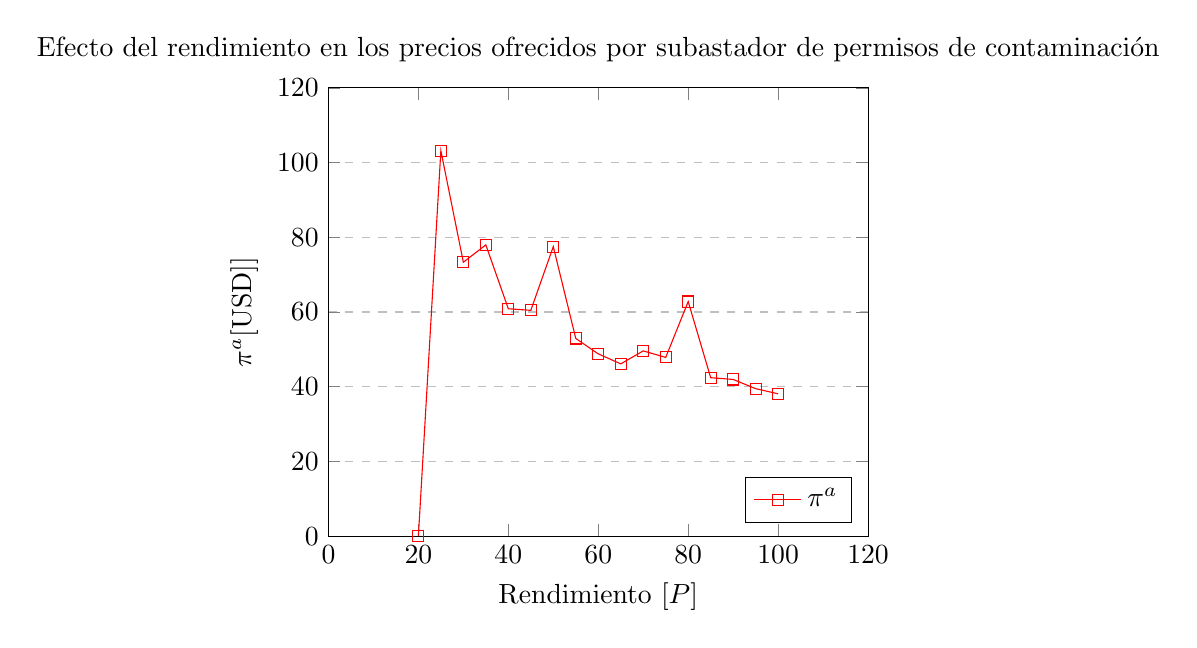
\begin{tikzpicture}
\begin{axis}[
    title={Efecto del rendimiento en los precios ofrecidos por subastador de permisos de contaminación},
    xlabel={Rendimiento [$P$]},
    ylabel={$\pi^a$[USD]]},
    xmin=0, xmax=120,
    ymin=0, ymax=120,
    xtick={0,20,40,60,80,100,120},
    ytick={0,20,40,60,80,100,120},
    legend pos=south east,
    ymajorgrids=true,
    grid style=dashed,
]

\addplot[
    color=red,
    mark=square,
    ]
    coordinates {
    (20,0)(25,103.196)(30,73.335)(35,77.973)(40,60.880)(45,60.448)(50,77.507)(55,52.927)(60,48.799)(65,46.123)(70,49.598)(75,47.855)(80,62.802)(85,42.426)(90,41.955)(95,39.492)(100,38.110)
    };
    \legend{$\pi^a$}
    
\end{axis}
\end{tikzpicture}

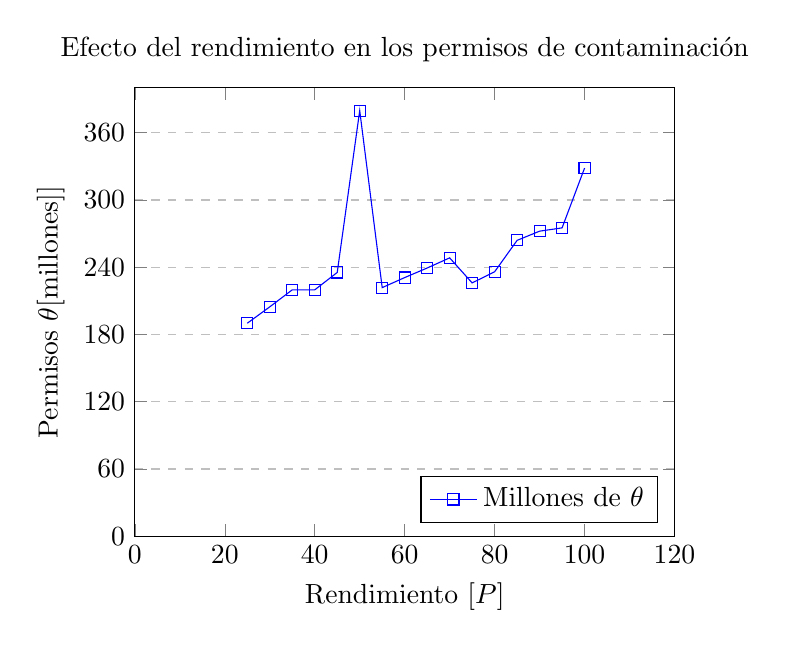
\begin{tikzpicture}
\begin{axis}[
    title={Efecto del rendimiento en los permisos de contaminación},
    xlabel={Rendimiento [$P$]},
    ylabel={Permisos $\theta$[millones]]},
    xmin=0, xmax=120,
    ymin=0, ymax=400,
    xtick={0,20,40,60,80,100,120},
    ytick={0,60,120,180,240,300,360},
    legend pos=south east,
    ymajorgrids=true,
    grid style=dashed,
]

\addplot[
    color=blue,
    mark=square,
    ]
    coordinates {
    (25,190)(30,204.63)(35,219.81)(40, 219.79)(45, 235.31)(50,379.72)(55,221.79)(60, 230.75)(65,239.28)(70,248.33)(75,225.99)(80,235.93 )(85,263.95)(90,272.16)(95,275.08)(100,328.44)
    };
    \legend{Millones de $\theta$}
    
\end{axis}
\end{tikzpicture}

\subsection{Adaptación modelo \textit{Profit Oriented}}

\begin{footnotesize}
\begin{equation}
\begin{array}{rrclcl}
   \displaystyle \min_{\theta} & -\theta \pi^aP + c(P-d)^2+F(\theta) \\\textrm{s.a.} \label{eq:profit2}\\
\end{array}
\end{equation}
\begin{equation}
\begin{array}{cl}
    \theta \pi^a P - c(P-d)^2 \geq 0 & (\eta)  \label{profit2:r1}
\end{array}
\end{equation}
\begin{equation}
\begin{array}{cl}
    \hat{\theta}\cdot(1+error)-\theta \geq 0 & (\mu)  \label{profit2:r2}
\end{array}
\end{equation}
\begin{equation}
\begin{array}{cl}
    \theta \geq 0 & (\varrho)
\end{array}
\end{equation}
\end{footnotesize}

La incorporación de la restricción \ref{profit2:r2}, tiene como fin restringir la emisión de permisos incorporando el CAP. Los permisos se acotan a que estos no pueden superar el CAP mas su error de cálculo explicado anteriormente.
\vspace{2.5mm}

$\hat{\theta}$ toma el valor del presupuesto de emisiones (CAP) impuesto por el gobierno. En esta misma restricción, se utiliza el valor error, el cuál representa el error de cálculo de este presupuesto, estimado por \cite{andres_new_2014}. Definiendo un $error=0,202$. 
\vspace{2.5mm}

Con esta nueva formulación, se calibra el modelo y posteriormente se resuelve.

\subsection{Calibración}

Para calibrar, se realiza el mismo procedimiento explicado anteriormente. 

\begin{table}[H]
    \centering
    \begin{tabular}{|l|l|l|l|l|l|}
    \hline
        c & $\pi^a$ & $\theta$ & $\pi^a$ original &  CAP& $\Delta \pi^a$  \\ \hline
         \$5  &  \$270.13  & 1.20E+08 &  \$315.83  & 1.00E+08 &  \$45.70   \\ \hline
         \$5,000  &  \$241.47  & 1.20E+08 &  \$315.83  & 1.00E+08 &  \$74.36   \\ \hline
         \$50,000  &  \$239.26  & 1.20E+08 &  \$315.83  & 1.00E+08 &  \$76.57   \\ \hline
         \$500,000  &  \$223.70  & 1.20E+08 &  \$315.83  & 1.00E+08 &  \$92.12   \\ \hline
         \$5,000,000  &  \$226.19  & 1.20E+08 &  \$315.83  & 1.00E+08 &  \$89.64   \\ \hline
         \$50,000,000  &  \$270.13  & 1.20E+08 &  \$315.83  & 1.00E+08 &  \$45.70   \\ \hline
         \$500,000,000  &  \$270.13  & 1.20E+08 &  \$315.83  & 1.00E+08 &  \$45.70   \\ \hline
         \$5,000,000,000  &  \$260.94  & 1.20E+08 &  \$315.83  & 1.00E+08 &  \$54.89   \\ \hline
         \$50,000,000,000  &  \$17.56  & 1.16E+08 &  \$315.83  & 1.00E+08 &  \$298.26   \\ \hline
         \$500,000,000,000  &  \$172.70  & 1.18E+08 &  \$315.83  & 1.00E+08 &  \$143.13   \\ \hline
         \$900,000,000,000  &  \$310.34  & 1.18E+08 &  \$315.83  & 1.00E+08 &  \$5.49   \\ \hline
         \$910,000,000,000  &  \$313.76  & 1.18E+08 &  \$315.83  & 1.00E+08 &  \$2.07   \\ \hline
         \$912,000,000,000  &  \$314.12  & 1.18E+08 &  \$315.83  & 1.00E+08 &  \$1.70   \\ \hline
         \$915,000,000,000  &  \$328.58  & 1.14E+08 &  \$315.83  & 1.00E+08 &  \$12.75   \\ \hline
         \$920,000,000,000  &  \$317.24  & 1.18E+08 &  \$315.83  & 1.00E+08 &  \$1.41   \\ \hline
         \$1,000,000,000,000  &  \$346.94  & 1.18E+08 &  \$315.83  & 1.00E+08 &  \$31.11   \\ \hline
         \$2,000,000,000,000  &  \$724.72  & 1.13E+08 &  \$315.83  & 1.00E+08 &  \$408.90   \\ \hline
         \$3,000,000,000,000  &  \$1,087.10  & 1.13E+08 &  \$315.83  & 1.00E+08 &  \$771.27   \\ \hline
         \$4,000,000,000,000  &  \$2,218.81  & 7.38E+07 &  \$315.83  & 1.00E+08 &  \$1,902.98   \\ \hline
    \end{tabular}
    \caption{{\footnotesize Calibración modelo Profit Oriented 2}}
    \label{calibracionPO2}
\end{table}

En el Cuadro \ref{calibracionPO2} se observa que existe un efecto lineal entre el costo $c$ y los precios $\pi^a$ a partir de los $\$50.000.000.000$ en costos. Esto se explica gracias a como este modelo está formulado: a mayor costo, se incurrirá a un mayor precio en los permisos para tener utilidades positivas. Antes del precio mencionado, los costos no son lo suficientemente altos como para afectar las ganancias.
\vspace{2.5mm}

Finalmente, con un costo $c= \$ 920,000,000,000$ se tiene la mejor aproximación al $\pi^a$ original. 
\vspace{2.5mm}

\subsection{Resultados}

En este modelo se incorpora el rendimiento como parámetro, por lo que se estudia como afecta las variables del modelo.
\vspace{2.5mm}

\begin{table}[H]
    \centering
    \begin{tabular}{|l|l|l|l|l|}
    \hline
        Rend[P]  & CAP & $\theta$  & $\frac{\theta}{CAP}$  & $\pi^a$  \\ \hline
        0.798  & 100,000,000  & 120,200,000 & 1.20  &  \$270.13   \\ \hline
        0.8  & 100,000,000 & 120,200,000 & 1.20  &  \$270.13   \\ \hline
        0.85  & 100,000,000 & 113,654,321 & 1.14  &  \$25.75   \\ \hline
        0.9  & 100,000,000 & 113,568,965 & 1.14  &  \$93.65   \\ \hline
        0.95  & 100,000,000 & 118,470,479 & 1.18  &  \$188.86   \\ \hline
        0.99  & 100,000,000 & 114,916,396 & 1.15  &  \$298.11   \\ \hline
        1  & 100,000,000 & 118,332,486 & 1.18  &  \$317.24   \\ \hline
    \end{tabular}
    \caption{{\footnotesize Efecto de $P$ en $\theta$ y $\pi^a$}}
    \label{efectopenthetapia}
\end{table}


En el Cuadro \ref{efectopenthetapia} se mantiene el presupuesto constante para entender el efecto del rendimiento en los permisos emitidos ($\theta$) y los precios establecidos por el subastador ($\pi^a$) al mantener constante el presupuesto de carbono (CAP). 
\vspace{2.5mm}

Por un lado, estos resultados muestran un efecto triangular en los permisos emitidos, con bajos rendimientos, se emite el máximo de permisos ($CAP + error$), en los rendimientos medios (0.85,0.9) se encuentra un mínimo de permisos emitidos y finalmente, con el rendimiento máximo, los permisos vuelven a subir cercano a $CAP + error$.
\vspace{2.5mm}

Por otro lado, existe un efecto similar en los precios $\pi^a$, encontrando valores máximos en los extremos del rendimiento.
\vspace{2.5mm}

De ambas observaciones se concluye que en los rendimientos 0.85 y 0.9 existe una inclinación a generar menores utilidades (menor ingresos debido al precio de permisos) y se busca un mejor bienestar social (se emiten menos permisos, o sea, se contamina menos).
\vspace{2.5mm}

Los resultados para todos los presupuesto de carbono se encuentran en el Cuadro \ref{efectopenthetapiatodoCAP} del Anexo \ref{anexoPO}.
\vspace{2.5mm}

\begin{table}[H]
    \centering
    \begin{tabular}{|l|l|l|l|l|}
    \hline
        Rend[P]  & CAP & $\theta$  & $\frac{\theta}{CAP}$  & $\pi^a$  \\ \hline
         0.8 & 100,000,000 & 120,200,000 & 1.20 &  \$270.13   \\ \hline
        0.8 & 200,000,000 & 240,400,000 & 1.20 &  \$60.57   \\ \hline
        0.8 & 300,000,000 & 360,600,000 & 1.20 &  \$119.47   \\ \hline
        0.8 & 400,000,000 & 454,798,037 & 1.14 &  \$95.83   \\ \hline
        0.8 & 500,000,000 & 601,000,000 & 1.20 &  \$79.31   \\ \hline
        0.8 & 600,000,000 & 605,279,899 & 1.01 &  \$66.57   \\ \hline
        0.8 & 700,000,000 & 605,279,899 & 0.86 &  \$56.37   \\ \hline
        0.8 & 800,000,000 & 961,600,000 & 1.20 &  \$152.50   \\ \hline
        0.8 & 900,000,000 & 605,279,899 & 0.67 &  \$42.26   \\ \hline
        0.8 & 1,000,000,000 & 605,279,899 & 0.61 &  \$35.98   \\ \hline
    \end{tabular}
    \caption{{\footnotesize Efecto del $CAP$ en $\theta$ y $\pi^a$}}
    \label{efectocapthetapia}
\end{table}
\vspace{2.5mm}

En el Cuadro \ref{efectocapthetapia} se muestra, manteniendo el rendimiento constante, el efecto del cambio del parámetro CAP en los permisos emitidos y los precios de permisos $\pi^a$.  Se observa que a mayor CAP existe un menor número de permisos emitidos relativos al CAP. En otras palabras, $\frac{\theta}{CAP}$ disminuye mientras mayor es el CAP establecido por el gobierno.
\vspace{2.5mm}

En adición a lo anterior, los precios $\pi^a$ tienen un comportamiento sinusoidal, tal vez ruido blanco, respecto al cambio en el CAP. Por un lado, se puede observar una tendencia a la baja para el precio mientras sube la cantidad de permisos (la ley de oferta y demanda espera esto ), pero, existen saltos extraños como en el CAP$=800MtCO_2$, donde se emiten muchos permisos y los precios aumentan. Estas anomalías pueden ser debido a que en estas ocasiones se invirtió más en información, traspasando los costos a la empresas que compran los permisos.
\vspace{2.5mm}

Los resultados para todos los rendimientos se encuentran en el Cuadro \ref{efectopenthetapiatodoCAP} del Anexo \ref{anexoPO}.
\vspace{2.5mm}

La Figura \ref{rendcap} muestra la relación entre la variación del CAP y el cociente de los permisos emitidos y el CAP para todos los rendimientos (recordar que en este modelo estos son parámetros).
\vspace{2.5mm}

\begin{figure}[H]
\centering
\resizebox{12cm}{10cm}{%
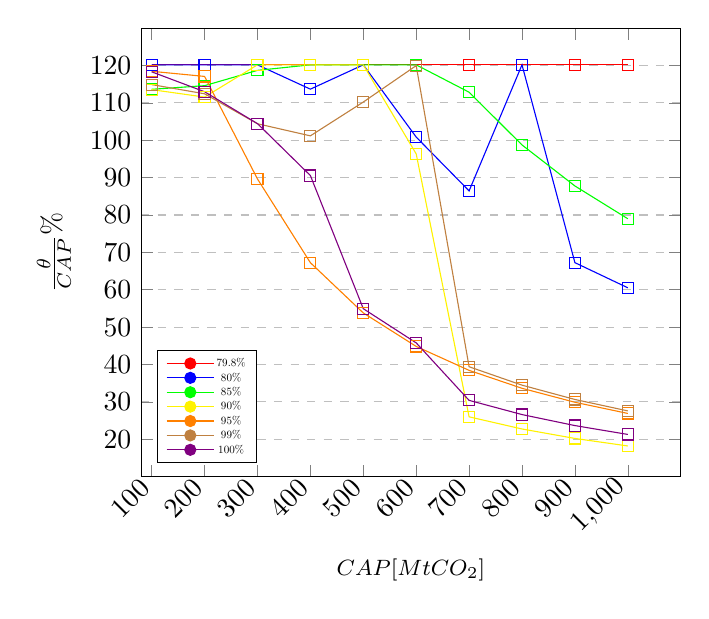
\begin{tikzpicture}
\centering
\begin{axis}[legend style={nodes={scale=0.4, transform shape}}, 
        legend image post style={mark=*},
    xlabel={{\footnotesize $CAP[MtCO_2]$}},
    ylabel={$\frac{\theta}{CAP}\%$},
    xmin=80, xmax=1100,
    ymin=10, ymax=130,
    xtick={100,200,300,400,500,600,700,800,900,1000},
    xticklabel style = {rotate=45,anchor=east},
    ytick={20,30,40,50,60,70,80,90,100,110,120},
    legend pos=south west,
    ymajorgrids=true,
    grid style=dashed,
]

\addplot[
    color=red,
    mark=square,
    ]
    coordinates {
    (100,120.2)(200,120.2)(300,120.2)(400,120.2)(500,120.2)(600,120.2)(700,120.2)(800,120.2)(900,120.2)(1000,120.2)
    };

\addplot[
    color=blue,
    mark=square,
    ]
    coordinates {
    (100,120.2)(200,120.2)(300,120.2)(400,113.69)(500,120.2)(600,100.87)(700,86.46)(800,120.2)(900,67.25)(1000,60.52)
    };
\addplot[
    color=green,
    mark=square,
    ]
    coordinates {
    (100,113.65)(200,114.62)(300,118.72)(400,120.2)(500,120.2)(600,120.2)(700,112.87)(800,98.76)(900,87.78)(1000,79)
    };
\addplot[
    color=yellow,
    mark=square,
    ]
    coordinates {
    (100,113.56)(200,111.57)(300,120.2)(400,120.2)(500,120.2)(600,96.37)(700,25.98)(800,22.73)(900,20.2)(1000,18.18)
    }; 
\addplot[
    color=orange,
    mark=square,
    ]
    coordinates {
    (100,118.47)(200,117.1)(300,89.66)(400,67.24)(500,53.79)(600,44.83)(700,38.42)(800,33.62)(900,29.88)(1000,26.89)
    };
\addplot[
    color=brown,
    mark=square,
    ]
    coordinates {
    (100,114.91)(200,112.45)(300,104.43)(400,101.19)(500,110.24)(600,119.99)(700,39.39)(800,34.46)(900,30.63)(1000,27.57)
    };
\addplot[
    color=violet,
    mark=square,
    ]
    coordinates {
    (100,118.33)(200,113)(300,104.46)(400,90.57)(500,54.93)(600,45.78)(700,30.39)(800,26.59)(900,23.64)(1000,21.27)
    };
    \legend{79.8\%, 80\%,85\%,90\%,95\%,99\%,100\%}  
\end{axis}

\end{tikzpicture}
}
\caption{{\footnotesize Rendimiento por CAP \textit{Profit Oriented}}}
\label{rendcap}
\end{figure}

Esta muestra que a mayor rendimiento mayor es la desviación de los permisos emitidos respecto al CAP. También se observa que a menor CAP, menor será la desviación de los permisos emitidos. 
\vspace{2.5mm}

Con lo anterior se concluye que mientras más se invierta en investigación, menor será la cantidad de permisos emitidos, esto puede ser respuesta a que el la información le indica que las emisiones deben disminuir. También, se cumple que mientras no exista inversión en información $P=d=0.798$, se emitirá el máximo de permisos posibles. Esto debido a que el subastador intentará maximizar sus ganancias.
\vspace{2.5mm}

\begin{figure}[H]
  \centering
  \begin{minipage}[b]{0.49\textwidth}
    \includegraphics[width=\textwidth]{docs/DocumentoMemoria/core/images/distribucion primera etapa.png}
    \caption{{\footnotesize Primera etapa y $P=80\%$}}
    \label{petapaPO}
  \end{minipage}
  \hfill
  \begin{minipage}[b]{0.49\textwidth}
    \includegraphics[width=\textwidth]{docs/DocumentoMemoria/core/images/distribucion segunda etapa.png}
    \caption{{\footnotesize Segunda etapa y $P=80\%$}}
    \label{setapaPO}
  \end{minipage}
\end{figure}

Para entender como este modelo afecta los permisos comprados por cada tecnología emisora de contaminante (al igual que el modelo original se consideran que estas son las empresas que usan Carbón, Gas y Petroleo como generador de electricidad), se grafican sus compras para cada cantidad de permisos emitidos (variando el CAP, manteniendo el rendimiento constante en $P=0.8$) en las figuras \ref{petapaPO} y \ref{setapaPO}.
\vspace{2.5mm}

En primer lugar, se grafica las distribuciones en la primera etapa, o sea, antes de que se revele el escenario de demanda energética en el futuro, en el cuál las empresas le compran los permisos al subastador. En segundo lugar, se grafica la nueva distribución para cada cantidad de permisos emitidos. Esta nueva distribución ocurre en la segunda etapa, donde las empresas forman un mercado de compra y venta de permisos entre ellas.
\vspace{2.5mm}

Por ejemplo, para un $CAP=100MtCO_2$, se emitieron 120 millones de permisos de contaminación. De los cuales el Gas compró un $61\%$ de esto, el Carbón un $32\%$ y el Petro Diesel un $7\%$. Luego, en la segunda etapa, estas tecnologías negociaron entre ellas (compras y ventas) y reajustaron su inversión en capacidad, llegando, finalmente, a que el GAS tiene un $67\%$ del total de permisos, el carbón un $33\%$ y el Petro Diesel vendió todos sus permisos. 
\vspace{2.5mm}

Estos resultados muestran que la dominancia (en cuanto a cantidad de permisos comprados) se mantiene estable entre etapas, siendo para casi todo presupuesto de carbono el Gas el mayor comprador. En adición a lo anterior, se ecuentra que para una emisión de 920 millones de permisos, existe una venta casi total de permisos. Esto no debería suceder ya que existe la restricción de condiciones de mercado \ref{rescom:2}, lo que puede significar que la alta no linealidad del modelo puede estar presentando errores para algunos valores o que existe la posibilidad de inclusión de recompra de permisos por parte del subastador, lo que permite disminuir las emisiones a pesar de existir una gran cantidad de permisos.
\vspace{2.5mm}

\begin{table}[H]
\begin{footnotesize}
    \centering
    \begin{tabular}{|l|l|l|l|l|l|l|l|l|l|l|}
    \hline
        $CAP$ & 100M & 200M & 300M & 400M & 500M & 600M & 700M & 800M & 900M & 1000M \\ \hline
        $\theta$  & 120M & 240M & 361M & 455M & 601M & 605M & 605M & 961M & 605M & 605M \\ \hline
        $\pi^d$  &  \$264.03   &  \$119.37   &  \$136.85   &  \$95.39   &  \$102.94   &  \$83.32   &  \$83.32   &  \$174.56   &  \$83.32   &  \$83.32   \\ \hline
    \end{tabular}
    \caption{{\footnotesize Precio de electricidad ($\pi^d$) por CAP y $P=80\%$}}
    \label{POpidporcap}
\end{footnotesize}
\end{table}

Una de las variables indirectas al modelo del subastador pero sobre la cual es importante estudiar el efecto de la reformulación del subastador es el precio de venta de electricidad que las empresas le cobran a las personas en el periodo 2018-2050. Su estudio puede entregar información valiosa sobre el bienestar social que estos nuevos modelos produzcan.
\vspace{2.5mm}

En el Cuadro \ref{POpidporcap} se encuentran los precios de electricidad $\pi^d$ ofrecido por las empresas generadoras de electricidad en el año 2018 (primera etapa) para todos los CAP y sus permisos emitidos resultantes. Los resultados muestran que mayores CAP resultan en menores precios de electricidad, a excepción del $CAP= 800MtCO_2$, en el cuál el precio es el segundo mayor de la tabla. Esto puede deberse a que, según lo mostrado en la Figura \ref{setapaPO}, las empresas generadoras contaminadoras, venden todos sus permisos en la segunda etapa, entonces, estas suben sus precios de venta de electricidad en la primera etapa.
\vspace{2.5mm}

\begin{figure}[H]
\centering
\resizebox{12cm}{9cm}{%
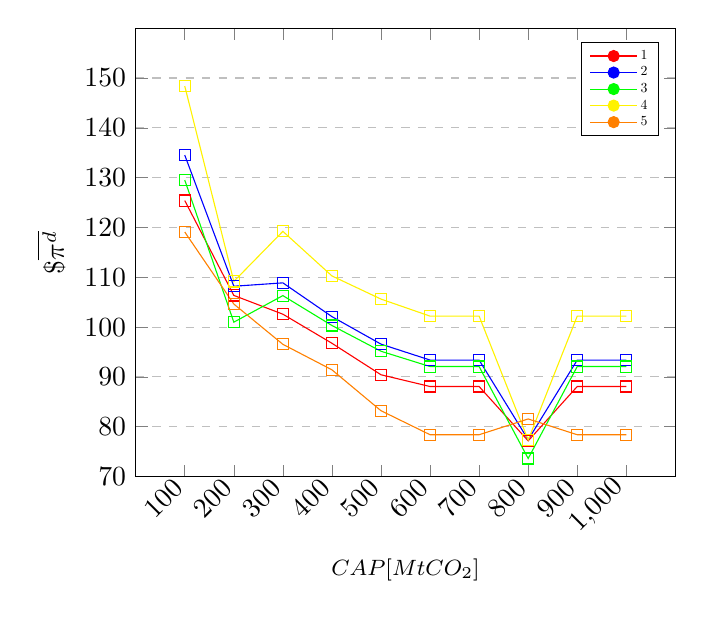
\begin{tikzpicture}
\centering
\begin{axis}[legend style={nodes={scale=0.5, transform shape}}, 
        legend image post style={mark=*},
    xlabel={{\footnotesize $CAP[MtCO_2]$}},
    xticklabel style = {rotate=45,anchor=east},
    ylabel={$\$ \overline{\pi^d}$},
    xmin=0, xmax=1100,
    ymin=70, ymax=160,
    xtick={100,200,300,400,500,600,700,800,900,1000},
    ytick={70,80,90,100,110,120,130,140,150},
    legend pos=north east,
    ymajorgrids=true,
    grid style=dashed,
]

\addplot[
    color=red,
    mark=square,
    ]
    coordinates {
    (100,125.4)(200,106.36)(300,102.59)(400,96.75)(500,90.43)(600,88.07)(700,88.07)(800,77.16)(900,88.07)(1000,88.07)
    };

\addplot[
    color=blue,
    mark=square,
    ]
    coordinates {(100,134.52)(200,108.2)(300,108.88)(400,102.1)(500,96.58)(600,93.38)(700,93.38)(800,77.39)(900,93.38)(1000,93.38)
    };
\addplot[
    color=green,
    mark=square,
    ]
    coordinates {
    (100,129.51)(200,100.99)(300,106.32)(400,100.32)(500,95.15)(600,92.08)(700,92.08)(800,73.62)(900,92.08)(1000,92.08)

    };
\addplot[
    color=yellow,
    mark=square,
    ]
    coordinates {
    (100,148.38)(200,109.17)(300,119.22)(400,110.27)(500,105.62)(600,102.2)(700,102.2)(800,77.33)(900,102.2)(1000,102.2)
    }; 
\addplot[
    color=orange,
    mark=square,
    ]
    coordinates {
    (100,119.09)(200,104.63)(300,96.54)(400,91.42)(500,83.21)(600,78.39)(700,78.39)(800,81.56)(900,78.39)(1000,78.39)
    };
    \legend{1,2,3,4,5}  
\end{axis}

\end{tikzpicture}
}

\caption{{\footnotesize Promedio de precios de electricidad (2019-2050)  por escenario}}
\label{pidcap}
\end{figure}

Finalmente, se comparan los precios promedio de electricidad en la segunda etapa (años 2019-2050) para cada uno de los escenarios del modelo en la Figura \ref{pidcap}, los cuales siguen la lógica de mayor precio por mayor demanda energética, pero se distingue una caída pronunciada en los precios para todos los escenarios cuando el $CAP=800MtCO_2$ . Esto puede deberse, como se muestra en el Cuadro \ref{efectocapthetapia}, a la alta emisión de permisos en ese periodo, resultando en una mayor producción por parte de las empresas contaminantes en comparación a las renovables.
\vspace{2.5mm}

Los escenarios, que pronostican la demanda eléctrica en los años mencionados anteriormente, son los mismos que en el modelo original, mostradas en la Figura \ref{fig:demandaescenarios}. 
\vspace{2.5mm}

El escenario 1 corresponde a un futuro de Chile con bajo PIB, el escenario 2 corresponde a un Chile con PIB medio, el escenario 3 corresponde a un Chile con electrificación, el escenario 4 corresponde a un PIB alto y el escenario 5 corresponde a alta intención de bajar uso eléctrico. 
\vspace{2.5mm}


\begin{figure}[H]
    \centering
    \includegraphics[width=10cm]{docs/DocumentoMemoria/core/images/demanda energetica segun escenario.png}
    \caption{{\footnotesize Demanda energética (Fuente: \protect\citeB{amigo_two_2021})}}
    \label{fig:demandaescenarios}
\end{figure}


\section{Modelo de Bienestar Social con tasa cuadrada}

Este modelo, explicado en el capítulo \ref{tasacuadrada}, es resuelto como un único MCP de problema de equilibrio de la siguiente forma:
\vspace{2.5mm}

\textbf{MCP productor}

Se repite el MCP del productor presente en el capítulo anterior \ref{resultadosprofit}.

\textbf{MCP condiciones de mercado}

Al igual que el productor, este es el mismo MCP de las condiciones de mercado presente en el Capítulo \ref{resultadosprofit}.

\textbf{MCP subastador}

\begin{tiny}
\begin{align}
    0 \leq \theta \perp - \pi^a + c(-2\theta + 2\hat{\theta})\frac{(2-2d-2(\frac{\theta - \hat{\theta}}{\hat{\theta}})^2)}{\hat{\theta}^2} - \eta \pi^a + c\eta((-2\theta + 2\hat{\theta})\frac{(2-2d-2(\frac{\theta - \hat{\theta}}{\hat{\theta}})^2)}{\hat{\theta}^2}) - \mu(\frac{-2\theta + 2\hat{\theta}}{\hat{\theta}^2}) - \lambda(\frac{2\theta-2\hat{\theta}}{\hat{\theta}^2}) \geq 0
\end{align}
\end{tiny}

\begin{footnotesize}
\begin{align}
    0 \leq \mu \perp 1 - \frac{(\theta-\hat{\theta})^2}{\hat{\theta}^2} - d  \geq 0\\
    0 \leq \lambda \perp \frac{(\theta-\hat{\theta})^2}{\hat{\theta}^2 }+ d \geq 0 \\
    0 \leq \eta \perp \theta \pi^a - c(1-\frac{(\theta - \hat{\theta})^2}{\hat{\theta}^2}-d)^2 \geq 0
\end{align}
\end{footnotesize}

\subsection{Calibración del modelo}

\begin{table}[H]
    \centering
    \begin{tabular}{|l|l|l|l|l|l|}
    \hline
        c & $\pi^a$ & $\theta$ & $\pi^a$ original &  CAP& $\Delta \pi^a$    \\ \hline
         \$1,000,000  &  \$51.76  & 3.02E+08 &  \$315.83  & 1.00E+08 &  \$264.07   \\ \hline
         \$10,000,000  &  \$212.84  & 1.63E+08 &  \$315.83  & 1.00E+08 &  \$102.98   \\ \hline
         \$100,000,000  &  \$220.51  & 1.55E+08 &  \$315.83  & 1.00E+08 &  \$95.31   \\ \hline
         \$109,000,000  &  \$142.81  & 9.10E+07 &  \$315.83  & 1.00E+08 &  \$173.02   \\ \hline
         \$9,000,000,000  &  \$181.21  & 1.98E+08 &  \$315.83  & 1.00E+08 &  \$134.62   \\ \hline
         \$9,500,000,000  &  \$184.11  & 1.97E+08 &  \$315.83  & 1.00E+08 &  \$131.72   \\ \hline
         \$9,900,000,000  &  \$232.82  & 1.45E+08 &  \$315.83  & 1.00E+08 &  \$83.01   \\ \hline
         \$9,999,000,000  &  \$232.82  & 1.45E+08 &  \$315.83  & 1.00E+08 &  \$83.01   \\ \hline
         \$9,999,005,000  &  \$207.55  & 1.69E+08 &  \$315.83  & 1.00E+08 &  \$108.27   \\ \hline
         \$9,999,500,000  &  \$232.82  & 1.45E+08 &  \$315.83  & 1.00E+08 &  \$83.01   \\ \hline
         \$9,999,900,000  &  \$182.38  & 1.98E+08 &  \$315.83  & 1.00E+08 &  \$133.45   \\ \hline
         \$10,000,000,000  &  \$182.27  & 1.95E+08 &  \$315.83  & 1.00E+08 &  \$133.56   \\ \hline
         \$90,000,000,000  &  \$146.83  & 1.54E+08 &  \$315.83  & 1.00E+08 &  \$168.99   \\ \hline
         \$100,000,000,000  &  \$211.29  & 1.57E+08 &  \$315.83  & 1.00E+08 &  \$104.54   \\ \hline
         \$110,000,000,000  &  \$144.07  & 1.52E+08 &  \$315.83  & 1.00E+08 &  \$171.76   \\ \hline
         \$150,000,000,000  &  \$164.89  & 1.51E+08 &  \$315.83  & 1.00E+08 &  \$150.93   \\ \hline
         \$200,000,000,000  &  \$143.18  & 1.49E+08 &  \$315.83  & 1.00E+08 &  \$172.65   \\ \hline
    \end{tabular}
    \caption{{\footnotesize Precio de electricidad ($\pi^d$) por CAP}}
    \label{calibracioncuadrado}
\end{table}

Los resultados de la calibración, en el Cuadro \ref{calibracioncuadrado}, muestran que el costo marginal $c$ con el cuál se tiene una variable $\pi^a$ más cercana al original (manteniendo un CAP de $100MtCO_{2}e$), es con un $c=\$9,900,000,000$.

\subsection{Resultados}

Contrario al anterior, en este modelo, el siguiente (Modelo con Precisión) y el original, el único parámetro que se varía para encontrar resultados es el presupuesto de carbono establecido por el gobierno (CAP). El rendimiento (P) se calcula con los valores de las variables encontradas.
\vspace{2.5mm}

Según lo explicado en el Capítulo \ref{tasacuadrada}, el rendimiento se calcula de las siguiente forma: 
\vspace{2.5mm}

\begin{equation}
\begin{array}{rrclcl}
\displaystyle P = 1- (\frac{{\theta - \hat{\theta}}}{\hat{\theta}})^2 \\
\end{array}
\end{equation}

Considerando lo anterior, se tienen los siguientes resultados:

\begin{table}[H]
    \centering
    \begin{tabular}{|l|l|l|l|l|}
    \hline
        CAP & $\theta$ & Rend[P] & $\frac{\theta}{CAP}$  & $\pi^a$  \\ \hline
        100,000,000 & 144,944,410  & 0.798  & 1.449  &  \$232.82   \\ \hline
        200,000,000 & 289,888,820  & 0.798  & 1.449  &  \$141.56   \\ \hline
        300,000,000 & 434,833,230  & 0.798  & 1.449  &  \$103.33   \\ \hline
        400,000,000 & 579,777,640  & 0.798  & 1.449  &  \$-   \\ \hline
        500,000,000 & 653,754,577  & 0.905  & 1.308  &  \$37.27   \\ \hline
        600,000,000 & 619,939,821  & 0.999  & 1.033  &  \$40.43   \\ \hline
        700,000,000 & 661,258,561  & 0.997  & 0.945  &  \$36.42   \\ \hline
        800,000,000 & 610,913,181  & 0.944  & 0.764  &  \$31.28   \\ \hline
        900,000,000 & 609,127,279  & 0.896  & 0.677  &  \$31.21   \\ \hline
        1,000,000,000 & 698,676,376  & 0.909  & 0.699  &  \$30.00   \\ \hline
    \end{tabular}
    \caption{{\footnotesize Resultados modelo tasa al cuadrado}}
    \label{resultadostasacuadrada}
\end{table}

El Cuadro \ref{resultadostasacuadrada}, muestra que este modelo entrega rendimientos variados para la mayoría de los CAP. A pesar de lo anterior, en los primeros cuatro CAP, el subastador prefiere no invertir en información $(P-d=0)$. También, presenta una caída sostenible de los precios mientras mayor es el CAP, existiendo eso si una anomalía en el cuarto CAP donde existe un precio de venta de permisos $pi^a=0$. Esto probablemente es debido a una falla en el modelo por su alta no linealidad o se debe buscar otra formulación del modelo para encontrar mejores resultados.
\vspace{2.5mm}

\begin{figure}[H]
\centering
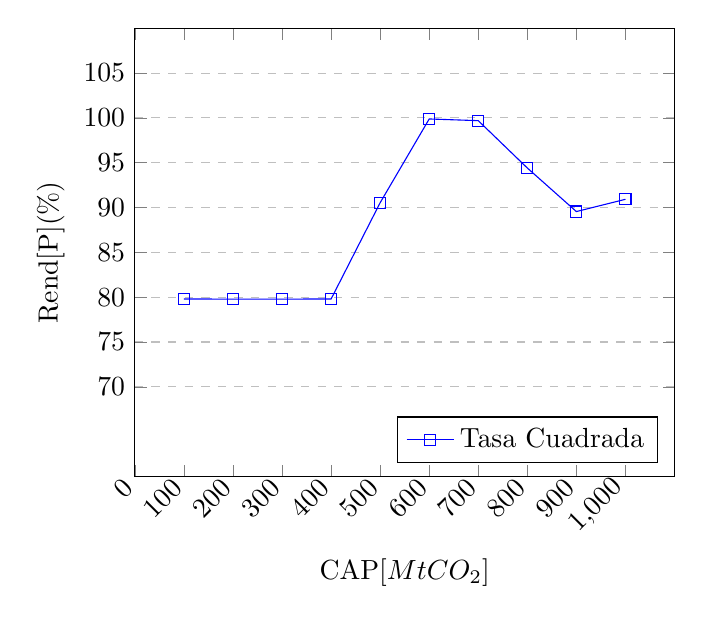
\begin{tikzpicture}
\begin{axis}[
    xlabel={CAP[$MtCO_2$]},
    ylabel={Rend[P](\%)},
    xmin=0, xmax=1100,
    ymin=60, ymax=110,
    xtick={0,100,200,300,400,500,600,700,800,900,1000},
    xticklabel style = {rotate=45,anchor=east},
    ytick={70,75,80,85,90,95,100,105},
    legend pos=south east,
    ymajorgrids=true,
    grid style=dashed,
]

\addplot[
    color=blue,
    mark=square,
    ]
    coordinates {
    (100,79.8)(200,79.79)(300,79.79)(400,79.8)(500,90.54)(600,99.88)(700,99.69)(800,94.41)(900,89.55)(1000,90.92)
    };
    \legend{Tasa Cuadrada}
    
\end{axis}
\end{tikzpicture}
\caption{{\footnotesize Efecto del CAP sobre P}}
\label{rendcapTC}
\end{figure}

Cuando se grafica el cambio del rendimiento en la Figura \ref{rendcapTC}, se observa un aumento de rendimiento entre los CAP 400 y 700, los cuales representan los escenarios donde existe una caída significativa a menor cociente $\frac{\theta}{CAP}$ según lo mostrado en la Figura \ref{rendcapTC2}.
\vspace{2.5mm}

Lo anterior, puede deberse a que mientras el subastador más invierte en información,entiende que menos se permisos de deben emitir para disminuir el costo social.
\vspace{2.5mm}

\begin{figure}[H]
\centering
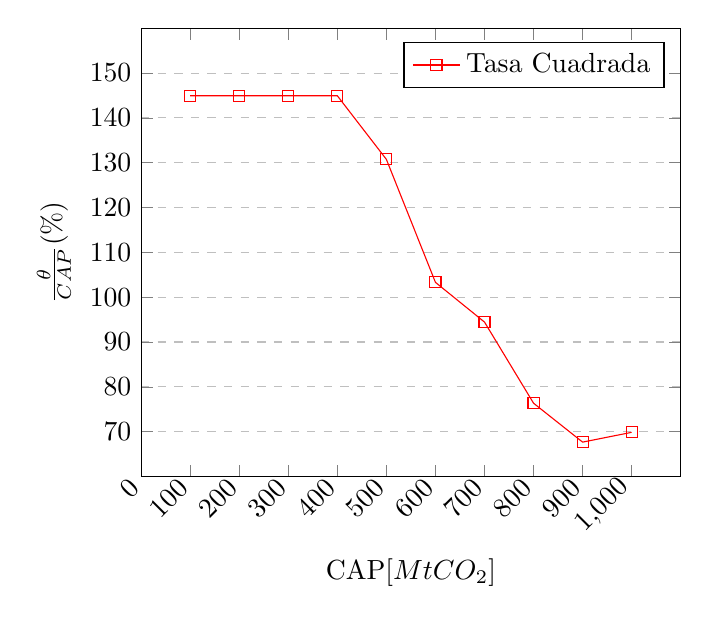
\begin{tikzpicture}
\begin{axis}[
    xlabel={CAP[$MtCO_2$]},
    ylabel={$\frac{\theta}{CAP}(\%)$},
    xmin=0, xmax=1100,
    ymin=60, ymax=160,
    xtick={0,100,200,300,400,500,600,700,800,900,1000},
    xticklabel style = {rotate=45,anchor=east},
    ytick={70,80,90,100,110,120,130,140,150},
    legend pos=north east,
    ymajorgrids=true,
    grid style=dashed,
]

\addplot[
    color=red,
    mark=square,
    ]
    coordinates {
    (100,144.94)(200,144.94)(300,144.94)(400,144.94)(500,130.75)(600,103.32)(700,94.46)(800,76.36)(900,67.68)(1000,69.86)
    };
    \legend{Tasa Cuadrada}
    
\end{axis}
\end{tikzpicture}
\caption{{\footnotesize Efecto del CAP sobre $\frac{\theta}{CAP}$}}
\label{rendcapTC2}
\end{figure}

En cuanto a la comparación de distribución de permisos entre las empresas contaminadoras, las figuras \ref{comptc1} y \ref{comptc2} muestras que, al igual que el modelo pasado, el Gas domina entre su competencia en la mayoría de los casos. 
\vspace{2.5mm}

A pesar de lo anterior, el Petro Diesel es el comprador mayoritario en los $CAP= 100$ y $CAP=200$ en la primera etapa. En la segunda etapa, estos venden casi todos sus permisos, entendiendo que lo hicieron como medida de inversión en corto plazo ya que con este modelo, probablemente los costos de producción son muy altos para bajas emisiones.
\vspace{2.5mm}

\begin{figure}[H]
  \centering
  \begin{minipage}[b]{0.49\textwidth}
    \includegraphics[width=\textwidth]{docs/DocumentoMemoria/core/images/distr primera etapa tasa cuadrada.png}
    \caption{{\footnotesize Distribución Primera Etapa}}
    \label{comptc1}
  \end{minipage}
  \hfill
  \begin{minipage}[b]{0.49\textwidth}
    \includegraphics[width=\textwidth]{docs/DocumentoMemoria/core/images/distr segunda etapa tasa cuadrada.png}
    \caption{{\footnotesize Distribución Segunda Etapa}}
    \label{comptc2}
  \end{minipage}
\end{figure}

Los precios de electricidad en la primera etapa resultantes, en el Cuadro \ref{TCpidporcap}, no muestran gran varianza entre los CAP 400 y 1000. Esto puede ser producto de que el subastador emite una cantidad similar de permisos en esos casos.
\vspace{2.5mm}

\begin{table}[H]
\begin{footnotesize}
    \centering
    \begin{tabular}{|l|l|l|l|l|l|l|l|l|l|l|}
    \hline
        CAP[$MtCO_2$] & 100 & 200 & 300 & 400 & 500 & 600 & 700 & 800 & 900 & 1000 \\ \hline
       $\theta$[Millones]  & 145  & 290  & 435  & 580  & 654  & 620  & 661  & 611  & 609  & 699  \\ \hline
        $\pi^d$  &  \$232.54   &  \$155.49   &  \$123.21   &  \$93.90   &  \$87.48   &  \$90.44   &  \$105.74   &  \$95.05   &  \$93.38   &  \$94.53   \\ \hline
    \end{tabular}
    \caption{{\footnotesize Precio de electricidad ($\pi^d$) en el año 2018 por CAP }}
    \label{TCpidporcap}
\end{footnotesize}
\end{table}


Finalmente, se comparan los promedios de precios de electricidad entre los años 2019-2050 para todos lo escenarios de demanda en la Figura \ref{TCrendcap}. Este modelo muestra consistencia en estos resultados ya que los precios para todos los escenarios se mueven consistentemente entre los CAP. Particularmente, se distingue un salto en los precios para todos los escenarios en el $CAP=700$, entregando información de que este puede no ser un modelo adecuado para altos CAP ya que produciría altos precios de electricidad para las personas. 

\begin{figure}[H]
\centering
\resizebox{12cm}{9cm}{%
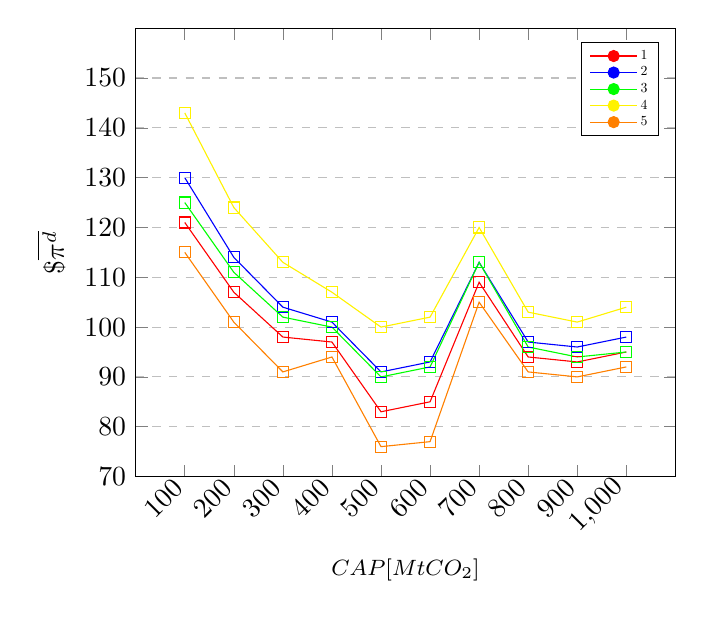
\begin{tikzpicture}
\centering
\begin{axis}[legend style={nodes={scale=0.5, transform shape}}, 
        legend image post style={mark=*},
    xlabel={{\footnotesize $CAP[MtCO_2]$}},
    xticklabel style = {rotate=45,anchor=east},
    ylabel={$\$ \overline{\pi^d}$},
    xmin=0, xmax=1100,
    ymin=70, ymax=160,
    xtick={100,200,300,400,500,600,700,800,900,1000},
    ytick={70,80,90,100,110,120,130,140,150},
    legend pos=north east,
    ymajorgrids=true,
    grid style=dashed,
]

\addplot[
    color=red,
    mark=square,
    ]
    coordinates {
    (100,121)(200,107)(300,98)(400,97)(500,83)(600,85)(700,109)(800,94)(900,93)(1000,95)
    };

\addplot[
    color=blue,
    mark=square,
    ]
    coordinates {(100,130)(200,114)(300,104)(400,101)(500,91)(600,93)(700,113)(800,97)(900,96)(1000,98)
    };
\addplot[
    color=green,
    mark=square,
    ]
    coordinates {
    (100,125)(200,111)(300,102)(400,100)(500,90)(600,92)(700,113)(800,96)(900,94)(1000,95)
    };
\addplot[
    color=yellow,
    mark=square,
    ]
    coordinates {
    (100,143)(200,124)(300,113)(400,107)(500,100)(600,102)(700,120)(800,103)(900,101)(1000,104)
    }; 
\addplot[
    color=orange,
    mark=square,
    ]
    coordinates {
   (100,115)(200,101)(300,91)(400,94)(500,76)(600,77)(700,105)(800,91)(900,90)(1000,92)
    };
    \legend{1,2,3,4,5}

\end{axis}
\end{tikzpicture}
}
\caption{{\footnotesize Precios de electricidad (2019-2050)  por escenario}}
\label{TCrendcap}
\end{figure}


\section{Modelo de Bienestar Social con precisión}

Esta versión, utilizando el concepto de precisión, se resuelve, al igual que los dos anteriores, como un problema de equilibrio en formato MCP:
\vspace{2.5mm}

\textbf{MCP productor}

Se repite el MCP del productor presente en el capítulo \ref{resultadosprofit}.

\textbf{MCP condiciones de mercado}

Al igual que del productor, este es el mismo MCP de la condiciones de mercado presente en el capítulo \ref{resultadosprofit}.

\textbf{MCP subastador}

\begin{footnotesize}
\begin{align}
    0 \leq \theta \perp -\pi^a   - \eta\pi^a  + \lambda -  \delta \geq 0\\
   0 \leq r \perp 2c\frac{(-1+d+\frac{r}{\hat{\theta}})}{\hat{\theta}} + 2c\eta \frac{(-1+d+\frac{r}{\hat{\theta}})}{\hat{\theta}} - \lambda - \delta  \geq 0\\
0 \leq \eta \perp \theta \pi^a - c(1-\frac{r}{\hat{\theta}}-d)^2 \geq 0 \\
0 \leq \lambda \perp r - \theta + \hat{\theta} \geq 0 \\
0 \leq \delta \perp r + \theta - \hat{\theta} \geq 0\\
0 \leq \mu \perp 1-\frac{r}{\hat{\theta}}-d \geq 0\\
0 \leq\chi \perp \frac{r}{\hat{\theta}} + d \geq 0 
\end{align}
\end{footnotesize}

\subsection{Calibración del modelo}

\begin{table}[H]
    \centering
    \begin{tabular}{|l|l|l|l|l|l|}
    \hline
          c & $\pi^a$ & $\theta$ & $\pi^a$ original &  CAP & $\Delta \pi^a$   \\ \hline
         \$50  &  \$244.34  & 1.20E+08 &  \$315.83  & 1.00E+08 & 71.482  \\ \hline
         \$500  &  \$219.60  & 1.20E+08 &  \$315.83  & 1.00E+08 & 96.229  \\ \hline
         \$5,000  &  \$209.14  & 1.20E+08 &  \$315.83  & 1.00E+08 & 106.689  \\ \hline
         \$50,000  &  \$219.41  & 1.20E+08 &  \$315.83  & 1.00E+08 & 96.415  \\ \hline
         \$500,000  &  \$213.10  & 1.20E+08 &  \$315.83  & 1.00E+08 & 102.723  \\ \hline
         \$3,000,000  &  \$205.23  & 1.20E+08 &  \$315.83  & 1.00E+08 & 110.593  \\ \hline
         \$3,500,000  &  \$198.96  & 1.20E+08 &  \$315.83  & 1.00E+08 & 116.864  \\ \hline
         \$3,900,000  &  \$218.76  & 1.20E+08 &  \$315.83  & 1.00E+08 & 97.067  \\ \hline
         \$4,000,000  &  \$270.13  & 1.20E+08 &  \$315.83  & 1.00E+08 & 45.699  \\ \hline
         \$4,000,001  &  \$194.42  & 1.20E+08 &  \$315.83  & 1.00E+08 & 121.405  \\ \hline
         \$4,000,005  &  \$270.13  & 1.20E+08 &  \$315.83  & 1.00E+08 & 45.699  \\ \hline
         \$5,000,000  &  \$270.13  & 1.20E+08 &  \$315.83  & 1.00E+08 & 45.699  \\ \hline
         \$6,000,000  &  \$212.54  & 1.20E+08 &  \$315.83  & 1.00E+08 & 103.286  \\ \hline
         \$50,000,000  &  \$270.13  & 1.20E+08 &  \$315.83  & 1.00E+08 & 45.699  \\ \hline
         \$500,000,000  &  \$270.13  & 1.20E+08 &  \$315.83  & 1.00E+08 & 45.699  \\ \hline
         \$5,000,000,000  &  \$270.13  & 1.20E+08 &  \$315.83  & 1.00E+08 & 45.699  \\ \hline
         \$50,000,000,000  &  \$237.74  & 1.20E+08 &  \$315.83  & 1.00E+08 & 78.09  \\ \hline
    \end{tabular}
    \caption{{\footnotesize Calibración modelo Precisión }}
    \label{calibracionprecision}
\end{table}

Los resultados de la calibración, en el Cuadro \ref{calibracionprecision}, muestran que el costo marginal $c$ con el cuál se tiene una variable $\pi^a$ más cercana al original (manteniendo un CAP de $100MtCO_{2}e$), es con un $c=\$4,000,000$.

\subsection{Resultados}

Según lo explicado en el Capítulo \ref{modeloconprecision}, el rendimiento se calcula de la siguiente forma: 
\vspace{2.5mm}

\begin{equation}
\begin{array}{rrclcl}
\displaystyle P = 1- \frac{r}{\hat{\theta}} \\
\end{array}
\end{equation}

Considerando lo anterior, se tienen los siguientes resultados:

\begin{table}[H]
    \centering
    \begin{tabular}{|l|l|l|l|l|}
    \hline
        CAP & $\theta$ & Rend[P] & $\frac{\theta}{CAP}$  & $\pi^a$ \\ \hline
        100,000,000 & 120,200,000  & 0.798  & 1.202  &  \$270.13   \\ \hline
        200,000,000 & 240,400,000  & 0.798  & 1.202  &  \$155.15   \\ \hline
        300,000,000 & 354,508,234  & 0.798  & 1.182  &  \$39.07   \\ \hline
        400,000,000 & 435,648,945  & 0.798  & 1.089  &  \$33.93   \\ \hline
        500,000,000 & 590,042,475  & 0.798  & 1.180  &  \$38.83   \\ \hline
        600,000,000 & 721,200,000  & 0.798  & 1.202  &  \$39.20   \\ \hline
        700,000,000 & 673,836,382  & 0.798  & 0.963  &  \$35.74   \\ \hline
        800,000,000 & 757,247,245  & 0.798  & 0.947  &  \$35.74   \\ \hline
        900,000,000 & 851,903,151  & 0.798  & 0.947  &  \$35.74   \\ \hline
        1,000,000,000 & 947,173,004  & 0.798  & 0.947  &  \$35.74   \\ \hline
    \end{tabular}
    \caption{{\footnotesize Resultados modelo Precisión}}
    \label{resultadosprecision}
\end{table}

En el Cuadro \ref{resultadosprecision} se distingue el rendimiento constante a lo largo de todos los CAP. Esto significa que el subastador encuentró como óptimo no invertir en información para disminuir el ruido. Para mejorar esto se debe formular de mejor forma la necesidad del subastador de sí invertir en información para aumentar el bienestar social. Esto se repite en todos lo modelos en diferentes niveles.
\vspace{2.5mm}

Como resultado de lo anterior, se entiende que existe espacio para mejorar los modelos y en especial para formular la atención racional enfocada en el subastador de una forma que este busque con mayor nivel el bienestar social. Una idea a seguir es la de encontrar la forma en que el error de cálculo de presupuesto se puede disminuir y asignarle esta tarea al subastador. Entonces mientras más se invierta en información, se estaría invirtiendo en disminuir el error de cálculo de presupuesto, lo que estaría buscando un mejor bienestar social.
\vspace{2.5mm}

La conclusión anterior se desarrolla con mayor detalle en los siguientes capítulos.
\vspace{2.5mm}


\begin{figure}[H]
\centering
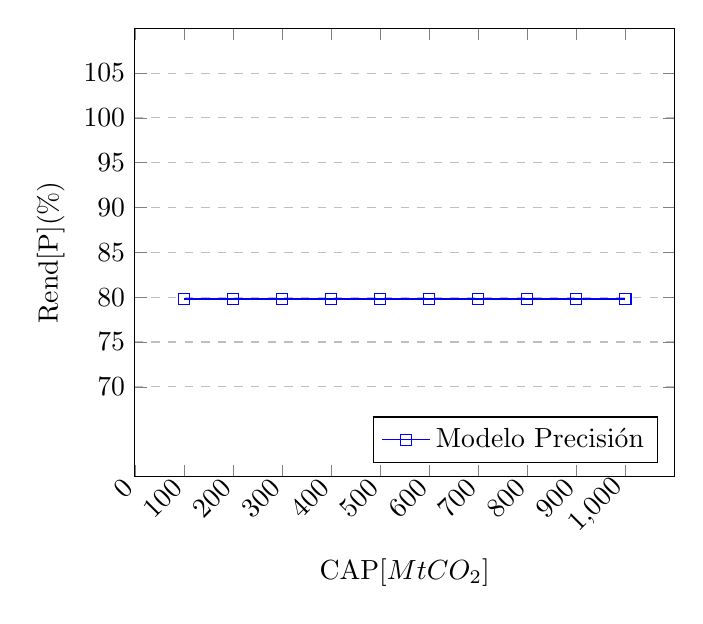
\begin{tikzpicture}
\begin{axis}[
    xlabel={CAP[$MtCO_2$]},
    ylabel={Rend[P](\%)},
    xmin=0, xmax=1100,
    ymin=60, ymax=110,
    xtick={0,100,200,300,400,500,600,700,800,900,1000},
    xticklabel style = {rotate=45,anchor=east},
    ytick={70,75,80,85,90,95,100,105},
    legend pos=south east,
    ymajorgrids=true,
    grid style=dashed,
]

\addplot[
    color=blue,
    mark=square,
    ]
    coordinates {
    (100,79.8)(200,79.8)(300,79.8)(400,79.8)(500,79.8)(600,79.8)(700,79.8)(800,79.8)(900,79.8)(1000,79.8)
    };
    \legend{Modelo Precisión}
    
\end{axis}
\end{tikzpicture}
\caption{{\footnotesize Efecto del CAP sobre P}}
\label{rendcapMP}
\end{figure}

La consistencia en los rendimientos, graficados en la Figura \ref{rendcapMP}, producen una disminución sostenida en los precios de los permisos $\pi^a$, sin saltos repentinos, pero si encontrando un límite inferior con un $CAP=700$.
\vspace{2.5mm}

En este modelo, como los otros, el cociente $\frac{\theta}{CAP}$, graficado en la Figura \ref{rendcapMP2}, disminuye mientras mayor es el CAP. Emitiendo cantidades similares a sus CAP ($\frac{\theta}{CAP} = 1$), producto de que el subastador no invierte en información, entonces este produce cercano al CAP propuesto.
\vspace{2.5mm}


\begin{figure}[H]
\centering
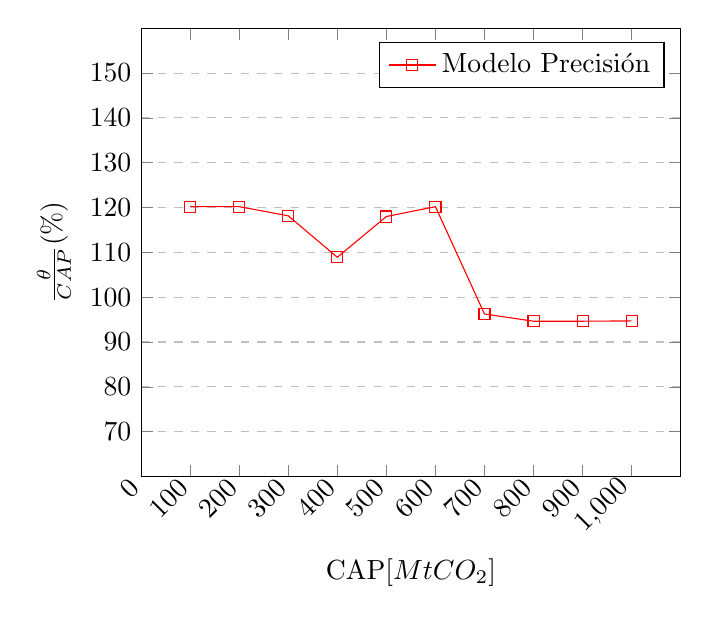
\begin{tikzpicture}
\begin{axis}[
    xlabel={CAP[$MtCO_2$]},
    ylabel={$\frac{\theta}{CAP}(\%)$},
    xmin=0, xmax=1100,
    ymin=60, ymax=160,
    xtick={0,100,200,300,400,500,600,700,800,900,1000},
    xticklabel style = {rotate=45,anchor=east},
    ytick={70,80,90,100,110,120,130,140,150},
    legend pos=north east,
    ymajorgrids=true,
    grid style=dashed,
]

\addplot[
    color=red,
    mark=square,
    ]
    coordinates {
    (100,120.2)(200,120.2)(300,118.16)(400,108.91)(500,118)(600,120.2)(700,96.26)(800,94.65)(900,94.65)(1000,94.71)
    };
    \legend{Modelo Precisión}
    
\end{axis}
\end{tikzpicture}
\caption{{\footnotesize Efecto del CAP sobre $\frac{\theta}{CAP}$}}
\label{rendcapMP2}
\end{figure}

La distribución de permisos entre las empresas contaminantes (figuras \ref{distriMP1} y \ref{distriMP3}) es similar al del modelo anterior, mostrando una dominancia del Gas.
\vspace{2.5mm}

Mientras que, en la segunda etapa, de forma progresiva, existen menos permisos que en el periodo anterior. Esto muestra que el modelo disminuye las emisiones a largo plazo.

\begin{figure}[H]
  \centering
  \begin{minipage}[b]{0.49\textwidth}
    \includegraphics[width=\textwidth]{docs/DocumentoMemoria/core/images/distr primera etapa precision.png}
    \caption{{\footnotesize Distribución Primera Etapa}}
    \label{distriMP1}
  \end{minipage}
  \hfill
  \begin{minipage}[b]{0.49\textwidth}
    \includegraphics[width=\textwidth]{docs/DocumentoMemoria/core/images/distr segunda etapa precision.png}
    \caption{{\footnotesize Distribución Segunda Etapa}}
     \label{distriMP3}
  \end{minipage}
\end{figure}

Los precios de electricidad en la primera (mostrados en el Cuadro \ref{Ppidporcap}), presentan una baja varianza entre los CAP 300 y 1000. Junto con el análisis realizado sobre la distribución de permisos, se anticipa que estos precios pueden no bajar cambiar mucho en la segunda etapa debido a que las empresas contaminadoras, las cuales producen electricidad más barata, venden gran parte de sus permisos.
\vspace{2.5mm}


\begin{table}[H]
\begin{footnotesize}
    \centering
    \begin{tabular}{|l|l|l|l|l|l|l|l|l|l|l|}
    \hline
       CAP[$MtCO_2$] & 100 & 200 & 300 & 400 & 500 & 600 & 700 & 800 & 900 & 1000 \\ \hline
          $\theta$[Millones] & 120 & 240 & 355 & 436 & 590 & 721 & 674 & 757 & 852 & 947 \\ \hline
    $\pi^d$  &  \$264.03   &  \$169.98   &  \$106.88   &  \$98.92   &  \$110.36   &  \$93.00   &  \$105.33   &  \$99.07   &  \$97.95   &  \$92.09   \\ \hline
    \end{tabular}
    \caption{{\footnotesize Precio de electricidad ($\pi^d$) en el año 2018 por CAP }}
    \label{Ppidporcap}
\end{footnotesize}
\end{table}

La Figura \ref{MPrendcap} confirma el análisis anterior, ya que los precios muestran una menor pendiente que los otros modelos para cada uno de los escenarios.
\vspace{2.5mm}

\begin{figure}[H]
\centering
\resizebox{12cm}{9cm}{%
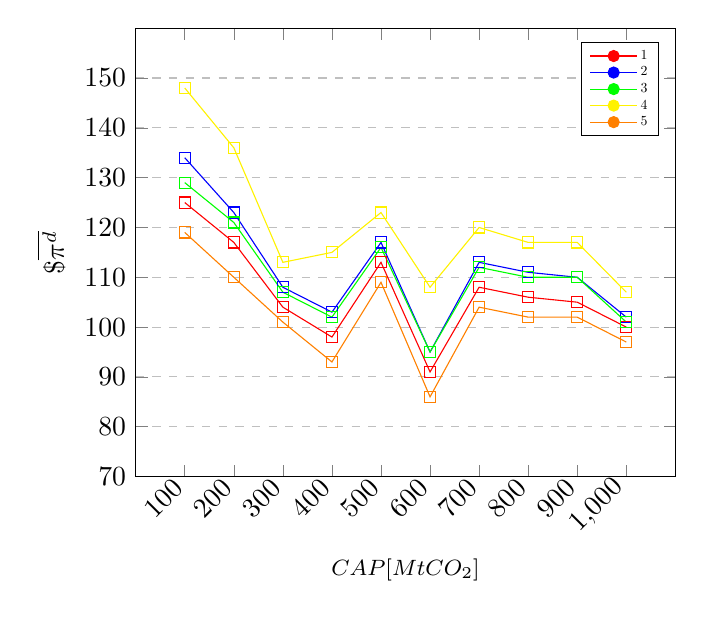
\begin{tikzpicture}
\centering
\begin{axis}[legend style={nodes={scale=0.5, transform shape}}, 
        legend image post style={mark=*},
    xlabel={{\footnotesize $CAP[MtCO_2]$}},
    xticklabel style = {rotate=45,anchor=east},
    ylabel={$\$ \overline{\pi^d}$},
    xmin=0, xmax=1100,
    ymin=70, ymax=160,
    xtick={100,200,300,400,500,600,700,800,900,1000},
    ytick={70,80,90,100,110,120,130,140,150},
    legend pos=north east,
    ymajorgrids=true,
    grid style=dashed,
]

\addplot[
    color=red,
    mark=square,
    ]
    coordinates {
    (100,125)(200,117)(300,104)(400,98)(500,113)(600,91)(700,108)(800,106)(900,105)(1000,100)
    };

\addplot[
    color=blue,
    mark=square,
    ]
    coordinates {(100,134)(200,123)(300,108)(400,103)(500,117)(600,95)(700,113)(800,111)(900,110)(1000,102)
    };
\addplot[
    color=green,
    mark=square,
    ]
    coordinates {
    (100,129)(200,121)(300,107)(400,102)(500,116)(600,95)(700,112)(800,110)(900,110)(1000,101)
    };
\addplot[
    color=yellow,
    mark=square,
    ]
    coordinates {
    (100,148)(200,136)(300,113)(400,115)(500,123)(600,108)(700,120)(800,117)(900,117)(1000,107)
    }; 
\addplot[
    color=orange,
    mark=square,
    ]
    coordinates {
    (100,119)(200,110)(300,101)(400,93)(500,109)(600,86)(700,104)(800,102)(900,102)(1000,97)
    };

    \legend{1,2,3,4,5}

\end{axis}
\end{tikzpicture}
}
\caption{{\footnotesize Precios de electricidad (2019-2050)  por escenario}}
\label{MPrendcap}
\end{figure}

\section{Comparación de Modelos}

Finalmente, se realiza una comparación entre todos los modelos creados en este trabajo y el modelo original de \citeB{amigo_two_2021}. La idea de esto es entender el efecto del subastador en sus utilidades,  en el bienestar social y entender si utilizar el efecto de atención racional mejora estos efectos. También, es una medida para entender el efecto particular de cada modelo. 
\vspace{2.5mm}

Esta es una primera aproximación de inclusión de atención racional en el subastador. Por lo tanto, para juzgar si la reformulación del modelo es efectiva en cuanto al aumento de bienestar social, se espera que una de estas versiones del modelo presente precios más bajos para las personas ($\pi^d$) en $40\%$ o más de los CAP o menos permisos emitidos en $40\%$ o más de los CAP.
\vspace{2.5mm}



\begin{figure}[H]
    \centering
    \includegraphics[width=12cm]{docs/DocumentoMemoria/core/images/utilidad de todos lo modelos.png}
    \caption{Utilidad del subastador por modelo }
    \label{utilidades}
\end{figure}

Las utilidades del subastador presentadas en la Figura \ref{utilidades}, muestran que en un $70\%$ de los presupuestos de carbono establecidos por el gobierno, el modelo original presenta las más altas ganancias. 
\vspace{2.5mm}

Por un lado, es importante mencionar que no se consideraron gastos para el subastador en este modelo ya que su función objetivo solo consideraba un costo llamado Costo Social del Carbón. El cuál fue despreciado en la solución del modelo de equilibrio ya que se consideró independiente de los permisos emitidos ($\theta$) por los autores originales. 
\vspace{2.5mm}

Por otro lado, los modelos reformulados toman los valores de los costos de información adicional por medio de la calibración del ellos con el original. Por lo que tomar en cuenta las utilidades del subastador para estos, tampoco es el indicador más importante a considerar. En un trabajo posterior, se espera calcular estos costos de forma real. 
\vspace{2.5mm}


\begin{figure}[H]
\centering
\resizebox{12cm}{9cm}{%
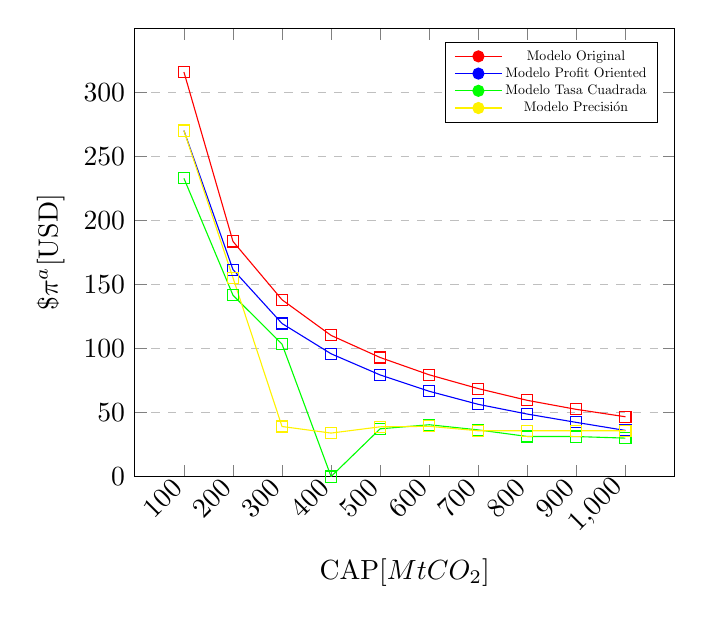
\begin{tikzpicture}
\centering
\begin{axis}[legend style={nodes={scale=0.5, transform shape}}, 
        legend image post style={mark=*},
    xlabel={CAP[$MtCO_2$]},
    ylabel={$\$ \pi^a$[USD]},
    xmin=0, xmax=1100,
    ymin=0, ymax=350,
    xtick={100,200,300,400,500,600,700,800,900,1000},
    xticklabel style = {rotate=45,anchor=east},
     ytick={0,50,100,150,200,250,300},
    legend pos=north east,
    ymajorgrids=true,
    grid style=dashed,
]

\addplot[
    color=red,
    mark=square,
    ]
    coordinates {
    (100,315.82)(200,183.55)(300,138.01)(400,110.18)(500,92.93)(600,79.42)(700,68.65)(800,59.48)(900,52.43)(1000,46.66)
    };

\addplot[
    color=blue,
    mark=square,
    ]
    coordinates {(100,270.12)(200,161.56)(300,119.47)(400,95.83)(500,79.31)(600,66.57)(700,56.37)(800,48.76)(900,42.26)(1000,35.98)

    };
    
\addplot[
    color=green,
    mark=square,
    ]
    coordinates {
    (100,232.82)(200,141.55)(300,103.32)(400,0)(500,37.26)(600,40.43)(700,36.41)(800,31.27)(900,31.21)(1000,30)

    };
    
\addplot[
    color=yellow,
    mark=square,
    ]
    coordinates {
    (100,270.12)(200,155.15)(300,39.06)(400,33.93)(500,38.82)(600,39.2)(700,35.73)(800,35.73)(900,35.73)(1000,35.73)


    }; 
    \legend{Modelo Original, Modelo Profit Oriented,Modelo Tasa Cuadrada,Modelo Precisión}

\end{axis}
\end{tikzpicture}
}
\caption{{\footnotesize Precio de venta de permisos $\pi^a$ por CAP}}
\label{piapormodelo}
\end{figure}

Los precios de venta de permisos son un indicador de la cantidad de permisos emitidos ya que estos obedecen a la ley de demanda. También, son un indicador de los costos asociados a la producción de permisos. La Figura \ref{piapormodelo} muestra que el modelo original presenta los mayores precios para todos los CAP. Esto puede ser un indicador de que los nuevos modelos buscan con mayor efecto el bienestar social, ya que, a pesar de que estos presentan costos de producción, igualmente no transfieren estos costos a los permisos, produciendo potencialmente menores costos de electricidad. 
\vspace{2.5mm}

Por el contrario, estos precios pueden ser producto de más permisos emitidos, y por ende, más emisiones en el medio ambiente.
\vspace{2.5mm}


\begin{figure}[H]
\centering
\resizebox{12cm}{9cm}{%
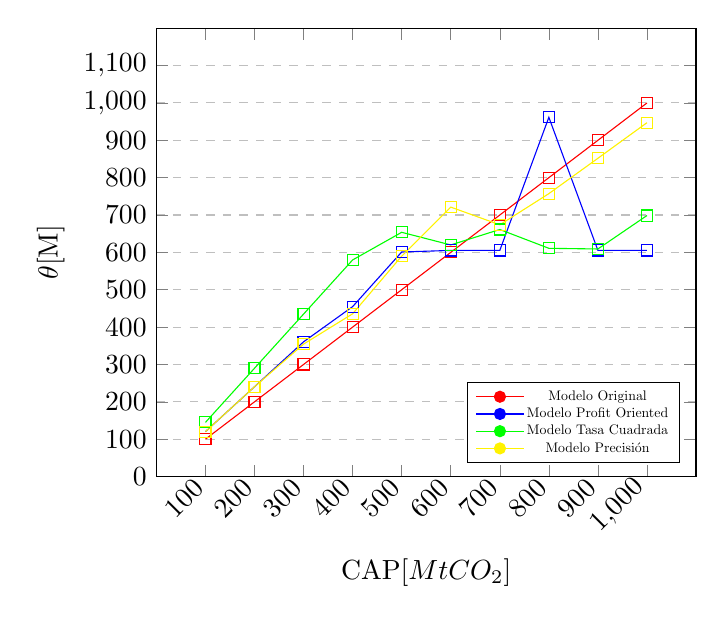
\begin{tikzpicture}
\centering
\begin{axis}[legend style={nodes={scale=0.5, transform shape}}, 
        legend image post style={mark=*},
    xlabel={CAP[$MtCO_2$]},
    ylabel={$\theta$[M]},
    xmin=0, xmax=1100,
    ymin=0, ymax=1200,
    xtick={100,200,300,400,500,600,700,800,900,1000},
    xticklabel style = {rotate=45,anchor=east},
    ytick={0,100,200,300,400,500,600,700,800,900,1000,1100},
    legend pos=south east,
    ymajorgrids=true,
    grid style=dashed,
]

\addplot[
    color=red,
    mark=square,
    ]
    coordinates {
    (100,100)(200,200)(300,300)(400,400)(500,500)(600,600)(700,700)(800,800)(900,900)(1000,1000)
    };

\addplot[
    color=blue,
    mark=square,
    ]
    coordinates {(100,120.2)(200,240.4)(300,360.6)(400,454.79)(500,601)(600,605.27)(700,605.27)(800,961.6)(900,605.27)(1000,605.27)
    };
    
\addplot[
    color=green,
    mark=square,
    ]
    coordinates {
    (100,144.94)(200,289.88)(300,434.83)(400,579.77)(500,653.75)(600,619.93)(700,661.25)(800,610.91)(900,609.12)(1000,698.67)
    };
    
\addplot[
    color=yellow,
    mark=square,
    ]
    coordinates {
    (100,120.2)(200,240.4)(300,354.5)(400,435.64)(500,590.04)(600,721.2)(700,673.83)(800,757.24)(900,851.9)(1000,947.17)
    }; 
    \legend{Modelo Original, Modelo Profit Oriented,Modelo Tasa Cuadrada,Modelo Precisión}

\end{axis}
\end{tikzpicture}
}
\caption{{\footnotesize Permisos emitidos por CAP}}
\label{permisospormodelo}
\end{figure}

La Figura \ref{permisospormodelo} muestra que el análisis anterior no es efectivo para todos los casos. En los primeros 5 CAP establecidos, el subastador en el modelo original emite menos permisos que las nuevas versiones, pero, en $CAP=600$ el modelo de Tasa Cuadrada emite una cantidad muy similar de permisos y en los siguientes,  emite menos permisos, resultando en menores emisiones. También, los otros dos modelos (Precisión y Profit Oriented) emiten menos permisos en 3 y 4 de los últimos 5 CAP respectivamente. 
\vspace{2.5mm}

Con lo anterior se cumple con los criterios mencionados al inicio de este sub capítulo para validar el uso de atención racional en este sistema ya que uno de los modelos tiene menos permisos emitidos en más de un $40\%$ de los CAP, pero lo más destacado es que todos los modelos presentan 3 o más CAP con menores emisiones.
\vspace{2.5mm}

\begin{figure}[H]
\centering
\resizebox{12cm}{9cm}{%
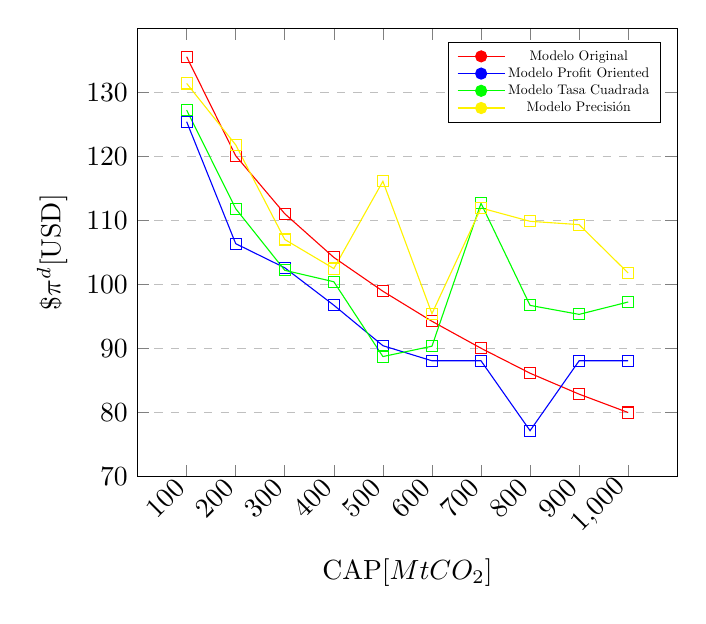
\begin{tikzpicture}
\centering
\begin{axis}[legend style={nodes={scale=0.5, transform shape}}, 
        legend image post style={mark=*},
    xlabel={CAP[$MtCO_2$]},
    ylabel={$\$ \pi^d$[USD]},
    xmin=0, xmax=1100,
    ymin=70, ymax=140,
    xtick={100,200,300,400,500,600,700,800,900,1000},
    xticklabel style = {rotate=45,anchor=east},
     ytick={70,80,90,100,110,120,130},
    legend pos=north east,
    ymajorgrids=true,
    grid style=dashed,
]

\addplot[
    color=red,
    mark=square,
    ]
    coordinates {
    (100,135.54)(200,120.08)(300,111.03)(400,104.21)(500,98.93)(600,94.24)(700,90.03)(800,86.13)(900,82.86)(1000,79.99)

    };

\addplot[
    color=blue,
    mark=square,
    ]
    coordinates {
    (100,125.4)(200,106.36)(300,102.59)(400,96.75)(500,90.43)(600,88.07)(700,88.07)(800,77.16)(900,88.07)(1000,88.07)

    };
    
\addplot[
    color=green,
    mark=square,
    ]
    coordinates {
    (100,127.22)(200,111.82)(300,102.2)(400,100.41)(500,88.73)(600,90.35)(700,112.66)(800,96.72)(900,95.32)(1000,97.25)
    };
    
\addplot[
    color=yellow,
    mark=square,
    ]
    coordinates {
    (100,131.38)(200,121.78)(300,107.01)(400,102.47)(500,116.1)(600,95.43)(700,111.93)(800,109.85)(900,109.33)(1000,101.77)
    }; 
    \legend{Modelo Original, Modelo Profit Oriented,Modelo Tasa Cuadrada,Modelo Precisión}

\end{axis}
\end{tikzpicture}
}
\caption{{\footnotesize Promedio precios de electricidad (2019-2050) $\pi^d$ por CAP}}
\label{pidpormodelo}
\end{figure}

Finalmente, se comparan los precios de electricidad para las personas entre los modelos en cada CAP. La Figura \ref{pidpormodelo} demuestra que los modelos Profit Oriented y Tasa Cuadrada crean menores precios para las personas en un $60\%$ de los CAP. Particularmente, el Profit Oriented lo logra en un $80\%$ de ellos. 
\vspace{2.5mm}

A pesar de que lo anterior es, en parte, producto de la cantidad emitida de permisos, se demuestra que estos modelos sí presentan un potencial de aumentar el bienestar social.

\chapter{Conclusiones y Recomendaciones}
\label{c5} % la etiqueta para referencias

Los resultados muestran que existe potencial para incorporar el concepto de atención racional en el modelo de \textit{cap and trade} de dos etapas, con el fin de aumentar el bienestar social. La comparación entre los modelos, realizada en el capítulo anterior, evidencia que los modelos nuevos entregan menor cantidad de permisos, menor precio de venta de estos y de electricidad en varios presupuestos de carbono establecidos por el gobierno.
\vspace{2.5mm}

Con el análisis anterior, se concluye que se cumplió el objetivo general de este trabajo. Se reformuló el sistema de \textit{cap and trade} de dos etapas creado por \citeB{amigo_two_2021} al incluir el concepto de atención racional satisfactoriamente, entregar resultados coherentes y con pruebas de potencialidad para crear un modelo reproducible en la realidad.
\vspace{2.5mm}

Sumado a lo anterior, se cumplieron todos los objetivos específicos y, adicionalmente, se incorporó y cumplió el objetivo de traducir el modelo al lenguaje de programación Julia. Esta traducción permitirá agilizar nuevas mejoras en el modelo. 
\vspace{2.5mm}

El concepto de atención racional se incorporó al subastador ya que este adquiere el rol de planificador social en el sistema. Él es quien, finalmente, será responsable de las emisiones generadas por las empresas eléctricas en el agregadp. Por lo tanto, tiene la capacidad de determinar la cantidad de permisos emitidos que mayor bienestar social produzcan.
\vspace{2.5mm}

Las dos versiones del modelo, \textit{Profit Oriented} y \emph{Welfare oriented} (modelo Tasa cuadrada y Precisión), demuestran que si el subastador incorpora la atención racional en su perfil de administrador,  disminuirá las emisiones de permisos en comparación con las propuestas por el gobierno (CAP), en especial mientras mayor sea el CAP. 
\vspace{2.5mm}

En el modelo original del subastador, este emite la cantidad de permisos que el CAP permite, sin tener un papel real en el modelo. Esta primera aproximación de incorporación de atención racional, no solo cambia su perfil, sino que también afecta sus utilidades al incorporar un gasto de inversión en información. Una recomendación para mejorar los modelos es que al subastador se le incorporen gastos de operación asociados con la fiscalización de las empresas emisoras y que este tenga un papel de compra de permisos y, tal vez, emisión de nuevos permisos en el largo plazo, si el escenario lo amerita.
\vspace{2.5mm}

Los trabajos realizados por \citeB{andres_new_2014} y \citeB{ballantyne_audit_2015} muestran que existe un error asociado con el cálculo del presupuesto de carbono establecido por Chile. Demuestran que este error se repite en la mayoría de los países, pero con algunas diferencias en su magnitud.
\vspace{2.5mm}

Debido a lo anterior, se realiza la recomendación principal de este trabajo: mejorar los modelos propuestos focalizando la atención racional en cómo los errores de cálculo de presupuestos pueden ser disminuidos. Con esto se debe, en primer lugar, entender de que forma se puede disminuir este error y qué costos implica. En segundo lugar, incorporarlo al modelo del subastador y formular el modelo en que la inversión en información genere un menor error. Finalmente, en esta formulación,  el subastador evaluará cuánto invertir en información, el número de permisos por emitir y el bienestar social como resultado de estas decisiones.





% Ingenieros prefieren la bibliografia antes que los anexos

\cleardoublepage

\addcontentsline{toc}{chapter}{Bibliografía}

\bibliographystyle{newapa}
\bibliography{references}

\appendix % seguido de archivos de apendices

\cleardoublepage

% Escribe 'Anexos' en el Indice General
\addcontentsline{toc}{chapter}{Anexos}

% anexo_a.tex

\chapter{Anexos}
\label{}



\section{Ejemplo Suma ponderada}\label{ej:sumapond}

Se tienen 3 escenarios posibles con $w = 1,2,3$ y parámetros $c_{w}= c_1,c_2,c_3$ y variables de diseño $x_{w}=x_{1}$, $x_{2}$,$x_{3}$. Luego, se tiene una suma ponderada de escenarios  $E_{\Theta}$[$x_{w}$ $c_{w}$] y la probabilidad de ocurrencia de cada escenario w es igual a $\Theta ={0.5 , 0.3 ,0.2 }$.
\vspace{2.5mm}

Con esto se tiene la siguiente expresión:

$$E_{\Theta} [ x_{w} c_{w}] = x_{1}c_{1}0.5 + x_{2}c_{2}0.3 + x_{3}c_{3}0.2 $$

\section{Parámetros Modelo Original}\label{anexo:parametros}


\section{Pruebas iniciales del rendimiento y atención racional en el subastador}\label{anexo:rendimiento}


Para realizar la evaluación del modelo, se realizará un gráfico con los resultados similar a la figura \ref{fig:fig6}. En esta se grafica la cantidad de permisos vendidos por el productor que produce energía con carbón y su influencia en el precio de mercado de los permisos. Esto representa el impacto que puede tener el modelo en eliminar el carbón como productor.

\begin{figure}[H]
    \centering
    \includegraphics[width=15cm]{docs/DocumentoMemoria/images/figura 6 amigo.png}
    \caption{Venta de permisos por generador de carbón (Fuente: \protect\citeB{amigo_two_2021})}
    \label{fig:fig6}
\end{figure}


\subsubsection{Modelo sin restricciones}

Primero se evaluará el modelo al considerar únicamente la función objetivo del subastador con el costo original $\mathcal{F}$ y el costo de rendimiento. También se considera como variable de decisión únicamente los permisos $\theta$.  

\begin{equation}
\begin{array}{rrclcl}
    \displaystyle \min_{\theta} & -\theta \pi^aP + \tilde{\mathcal{F}}(P)+F(\theta)  \label{fo:perfornorest}\\
\end{array}
\end{equation}
\begin{equation}
\begin{array}{cl}
    \theta \geq 0 & (\varrho)\label{res:sub2}
\end{array}
\end{equation}

Con lo anterior se logra el siguiente Lagrangiano:

$$\mathcal{L}(\theta)=-P\theta\pi^a+\mathcal{F}(\theta)+c(P-d)^2 - \varrho\theta $$

Realizando la derivada de primer orden para $\theta$ se obtiene:

\begin{equation}
\begin{array}{rrclcl}
    \frac{\partial\mathcal{L}(\theta)}{\partial (\theta)}=-P\pi^a+\frac{\partial\mathcal{F}(\theta)}{\partial(\theta)}-\varrho=0 \label{lag1}\\
\end{array}
\end{equation}
\begin{equation}
\begin{array}{rrclcl}
    \rightarrow -P\pi^a+\frac{\partial\mathcal{F}(\theta)}{\partial(\theta)}=\varrho \label{lag1}\\
\end{array}
\end{equation}
Con esto se obtiene la siguiente complementariedad para el problema del subastador:

\begin{equation}
\begin{array}{rrclcl}
    0\leq -P\pi^a+\frac{\partial\mathcal{F}(\theta)}{\partial(\theta)}\perp \theta \geq 0 \label{compllag1}\\
\end{array}
\end{equation}

Al igual que en el modelo original de \citeB{amigo_two_2021}, se consideran los siguientes valores para constantes y parámetros:
\begin{enumerate}
    \item $\frac{\partial\mathcal{F}(\theta)}{\partial(\theta)}=0$
    \item $CAP\sim \mathcal{N}(100MtCO_{2}e,0)$
\end{enumerate}

Con esto, al correr el modelo en el \textit{solver}, cambiando únicamente el valor del rendimiento ($P$), se encontraron los siguientes resultados:

\begin{table}[H]
\centering
\begin{tabular}{|l|l|l|}
\hline
\textbf{P($\%$)} & \textbf{$\theta$ (millones)} & \textbf{$\pi^a$($\frac{\$}{\theta}$)} \\ \hline
0 & N/A & N/A \\ \hline
5 & 104 & 223 \\ \hline
10 & 3203 & 0 \\ \hline
15 & 3203 & 0 \\ \hline
20 & 3203 & 0 \\ \hline
25 & 3203 & 0 \\ \hline
30 & 3203 & 0 \\ \hline
35 & 3203 & 0 \\ \hline
40 & 3203 & 0 \\ \hline
45 & 3203 & 0 \\ \hline
50 & 3203 & 0 \\ \hline
55 & 3203 & 0 \\ \hline
60 & 3203 & 0 \\ \hline
65 & 3203 & 0 \\ \hline
70 & 3203 & 0 \\ \hline
75 & 3203 & 0 \\ \hline
80 & 3203 & 0 \\ \hline
85 & 3203 & 0 \\ \hline
90 & 3203 & 0 \\ \hline
95 & 3203 & 0 \\ \hline
100 & 1870 & 0 \\ \hline
\end{tabular}
\caption{Resultados con rendimiento y sin restricciones}
\label{tabla:sinrestr}
\end{table}


Los resultados encontrados en el Cuadro \ref{tabla:sinrestr}, pueden ser resultado de no considerar una restricción para $\theta$ respecto al presupuesto de carbono en el problema del subastador. En la siguiente subsección se desarrolla el problema incluyendo la restricción adicional.

\subsubsection{Modelo con restricción original}

Manteniendo la restricción original de \citeB{amigo_two_2021} mostrada en \ref{res:sub1}. Se tiene el siguiente modelo:

\begin{equation}
\begin{array}{rrclcl}
   \displaystyle \min_{\theta} & -\theta \pi^aP + c(P-d)^2+F(\theta) \\\textrm{s.a.} \label{eq:perforconrestr}\\
\end{array}
\end{equation}
\begin{equation}
\begin{array}{cl}
    \varphi^-1 (\varepsilon )\sigma + \mu - \theta \geq 0 & (\eta)  \label{perforconrestr:r1}
\end{array}
\end{equation}
\begin{equation}
\begin{array}{cl}
    \theta \geq 0 & (\varrho)
\end{array}
\end{equation}

Al igual que el caso anterior, se debe convertir este modelo en un MCP. Para esto se aplican las condiciones de KKT.

$$\mathcal{L}(\theta)=-P\theta\pi^a+\mathcal{F}(\theta)+c(P-d)^2 -\eta(\varphi^-1 (\varepsilon )\sigma + \mu - \theta)- \varrho\theta $$

Realizando la derivada de primer orden para $\theta$ se obtiene:

\begin{equation}
\begin{array}{rrclcl}
    \frac{\partial\mathcal{L}(\theta)}{\partial (\theta)}=-P\pi^a+\frac{\partial\mathcal{F}(\theta)}{\partial(\theta)}-\eta -\varrho=0 \label{lag20}\\
\end{array}
\end{equation}
\begin{equation}
\begin{array}{rrclcl}
    \rightarrow -P\pi^a+\frac{\partial\mathcal{F}(\theta)}{\partial(\theta)}-\eta=\varrho \label{lag21}\\
\end{array}
\end{equation}

Obteniendo la primera complementariedad:

\begin{equation}
\begin{array}{rrclcl}
    0\leq -P\pi^a+\frac{\partial\mathcal{F}(\theta)}{\partial(\theta)}-\eta \perp \theta \geq 0 \label{compllag2}\\
\end{array}
\end{equation}

La segunda complementariedad se obtiene al considera la restricción \ref{perforconrestr:r1} con su variable dual respectiva $\eta$. Obteniendo:

\begin{equation}
\begin{array}{rrclcl}
    0 \leq \varphi^-1 (\varepsilon )\sigma + \mu - \theta \perp \eta \geq 0 \label{compllag2}\\
\end{array}
\end{equation}

Nuevamente, al igual que en el modelo original de \citeB{amigo_two_2021}, se consideran los siguientes valores para constantes y parámetros:
\begin{enumerate}
    \item $\frac{\partial\mathcal{F}(\theta)}{\partial(\theta)}=0$
    \item $CAP\sim \mathcal{N}(100MtCO_{2}e,0)$
\end{enumerate}

Con esto, al correr el modelo en el \textit{solver}, cambiando únicamente el valor del rendimiento ($P$), se encontraron los siguientes resultados:

\begin{table}[H]
\centering
\begin{tabular}{|l|l|l|}
\hline
\textbf{P($\%$)} & \textbf{$\theta$ (millones)} & \textbf{$\pi^a$($\frac{\$}{\theta}$)} \\ \hline
0 & 0.3336 & 30130 \\ \hline
5 & 100 & 315.825 \\ \hline
10 & 100 & 315.825 \\ \hline
15 & 100 & 315.825 \\ \hline
20 & 100 & 315.825 \\ \hline
25 & 100 & 315.825 \\ \hline
30 & 100 & 315.825 \\ \hline
35 & 100 & 315.825 \\ \hline
40 & 100 & 315.825 \\ \hline
45 & 100 & 315.825 \\ \hline
50 & 100 & 315.825 \\ \hline
55 & 100 & 315.825 \\ \hline
60 & 100 & 315.825 \\ \hline
65 & 100 & 315.825 \\ \hline
70 & 100 & 315.825 \\ \hline
75 & 100 & 315.825 \\ \hline
80 & 100 & 315.825 \\ \hline
85 & 100 & 315.825 \\ \hline
90 & 100 & 315.825 \\ \hline
95 & 100 & 315.825 \\ \hline
100 & 100 & 315.825 \\ \hline
\end{tabular}
\caption{Resultados con rendimiento y restricción original}
\label{tabla:conrestr}
\end{table}

Del Cuadro \ref{tabla:conrestr} se entiende que al incluir únicamente las restricciones del problema original solo existe un efecto en el precio y cantidad de permisos cuando el rendimiento es 0. Pero esto no debería ocurrir ya que por lo menos se tiene la información pública $d$. Cabe notar que una cantidad de $100 MtCO_2 e$ con un precio de 315.825 USD cada una, son los valores de resolución del problema original con los mismos parámetros. Este resultado puede resultar debido a que no se a incluido una restricción que describa de mejor forma el costo de rendir.

\section{GAMS de Amigo et al. (2021)}\label{anexo:GAMScomp}
\subsection{MCP del Productor}

\subsubsection{Derivada parcial respecto a $x_i(0)$}

En el código GAMS , se escribió la kkt de esta complementariedad de la siguiente forma en la línea 654:
\begin{verbatim}
kkt_x_first_producer(i).. Inv(i)*(1+percent(i)) + sum(w, psi(i,w))- CF(i)*t_year
*sum(w, sum( tau2,alpha(i,w,tau2))) - xi(i)=g=0;
\end{verbatim}
Siendo xi(i) la variable dual $\xi_i$ . Donde esta kkt se complementa con la variable respectiva $x_i(0)$ en la línea 724 del código.
\begin{verbatim}
kkt_x_first_producer.x_first
\end{verbatim}

\subsubsection{Derivada parcial respecto a $x_i(t,\omega)$}

Al igual que en el caso anterior, el código mantiene la variable dual, se puede ver en la línea 657 del código el KKT respectivo:

\begin{verbatim}
kkt_x_second_producer(i,tau2,w).. ((1/(1+R))**(ord(tau2)))*Prob(w)*Inv(i)*
(1+percent(i))*TCR(i,tau2)- CF(i)*t_year*sum(tau3$(tauAlpha_i(i,tau2,
tau3)),alpha(i,w,tau3)) + psi(i,w) -varphi(i,w,tau2)  =g=0;
\end{verbatim}

Con varphi(i,w,tau2) como la variable dual mencionada $\varphi_{i,\omega,t}$. 

\subsubsection{Derivada parcial respecto a $Q_i(0)$}

Como en los anteriores, en el código no se despeja la variable dual $\lambda_i$, se mantiene y se programa el MCP respectivo con la variable $Q_i(0)$. Se puede ver en la línea 660 del código de la siguiente forma:

\begin{verbatim}
kkt_q1_producer(i,tau).. (int(i)+C(i)*Q_first(i,tau))-pi_d(tau) + kappa(i,tau) - 
lambda(i,tau)+sum(w,gamma(i,w)*epsilon(i))=g= 0;
\end{verbatim}

Programando la complementariedad en la línea 728:

\begin{verbatim}
kkt_q1_producer.Q_first    
\end{verbatim}

\subsubsection{Derivada parcial respecto a $Q_i(t,\omega)$}

La línea 662 del código completa la kkt de la siguiente forma: 

\begin{verbatim}
kkt_qtau_producer(i,tau2,w).. 
((1/(1+R))**(ord(tau2)))*Prob(w)*((TC(i,tau2)*(int(i)+C(i)*Q_second(i,tau2,w)))- 
\end{verbatim}
\begin{verbatim}
pi2_d(tau2,w))+alpha(i,w,tau2)+gamma(i,w)*epsilon(i)-delta(i,tau2,w) =g= 0;
\end{verbatim}

Con la complementariedad escrita de la siguiente forma en la línea 729 del código:
\begin{verbatim}
kkt_qtau_producer.Q_second    
\end{verbatim}

\subsubsection{Derivada parcial respecto a $A_i(t)$}

En el código se tiene lo siguiente en la línea 664:
\begin{verbatim}
   kkt_A_producer(i).. pi_a - sum(w, beta(i,w)) - sum(w, gamma(i,w))=g= 0 
\end{verbatim}

Y efectuando la complementariedad en la línea 730:
\begin{verbatim}
    kkt_A_producer.A
\end{verbatim}

\subsubsection{Derivada parcial respecto a $V_i(w)$}
Programando la kkt en el código en la línea 667:
\begin{verbatim}
    kkt_V_producer(i,w)..  -Prob(w)*pi_v(i,w)+beta(i,w)+gamma(i,w)=g= 0
\end{verbatim}

Completando la complementariedad en la línea 731:
\begin{verbatim}
    kkt_V_producer.V
\end{verbatim}

\subsubsection{Derivada parcial respecto a $P_i(w)$}

Programando la kkt en el código en la línea 670:
\begin{verbatim}
    kkt_P_producer(i,j,w)$(ord(j) <> ord(i))..      Prob(w)* pi_v(j,w)-gamma(i,w) =g= 0
\end{verbatim}

Completando la complementariedad en la línea 732:
\begin{verbatim}
    kkt_P_producer.P  
\end{verbatim}

\subsubsection{Completando el problema del productor}

Las cuales se encuentran programadas entre las líneas 609 y 703 del código:

\begin{verbatim}
    capacity_stage_2_xnext(i,w,tau2).. CF(i)*t_year*(sum(tau3$(tau3_i(i,tau2,tau3)),
    x_next(i,tau3,w))+x_first(i)+Q_barT2(i,tau2) +Q_bar(i))-Q_second(i,tau2,w) =g=0;
\end{verbatim}
\begin{verbatim}
    capacity_stage_1(i,tau)..  CF(i)*t_year*Q_bar(i)- Q_first(i,tau) =g=0;
\end{verbatim}
\begin{verbatim}
    trading_permits(i,w)..  A(i)-V(i,w) =g= 0;
\end{verbatim}
\begin{verbatim}
    total_allowances(i,w)..  A(i) + sum(j$(ord(j) <> ord(i)),P(i,j,w))-V(i,w) - 
    sum(tau2,Q_second(i,tau2,w)*epsilon(i)) - sum(tau,Q_first(i,tau)*epsilon(i))   
    =g= 0;
\end{verbatim}
\begin{verbatim}
    resource_potential(i,w)..   -Q_bar(i) - x_first(i) - sum(tau3,x_next(i,tau3,w))+
    sum(tau2,Q_barT2(i,tau2)) + RP(i) =g= 0;
\end{verbatim}

Existiendo sus complementariedades entre las líneas 734 y 744:

\begin{verbatim}
    capacity_stage_1.kappa
    capacity_stage_2_xnext.alpha
    resource_potential.psi
    trading_permits.beta
\end{verbatim}

\subsection{MCP condiciones de mercado}

\subsubsection{Restricción de permisos disponibles}
En el código se encuentra la restricción y complementariedad en las líneas 708 y 751 respectivamente: 
\begin{verbatim}
    kkt_A_theta..    theta - sum(i,A(i))=e= 0;
    kkt_A_theta.pi_a
\end{verbatim}

\subsubsection{Restricción de equilibrio en el mercado de compra y venta de permisos}
En el código se encuentra la restricción y complementariedad en las líneas 713 y 752 respectivamente: 
\begin{verbatim}
    kkt_P_V(i,w).. V(i,w)=e=sum(j$(ord(j) <> ord(i)),P(j,i,w));
    kkt_P_V.pi_v 
\end{verbatim}

\subsubsection{Abastecimiento de demanda en la primera etapa}
\begin{verbatim}
    kkt_Q_D_first(tau).. sum(i,Q_first(i,tau))=e=D1(tau);
    kkt_Q_D_first.pi_d
\end{verbatim}

\subsubsection{Abastecimiento de demanda en la segunda etapa}
En el código se encuentra la restricción y complementariedad en las líneas 711 y 754 respectivamente: 
\begin{verbatim}
    kkt_Q_D_second(tau2,w)..sum(i,Q_second(i,tau2,w))=e=D2(w,tau2);
    kkt_Q_D_second.pi2_d
\end{verbatim}    % archivo de apendice

%\input{apendice_b}    % otro archivo de apendice

\label{end}
\end{document}

%%%%%%%%%%%%%%%%%%%%%%%%%%%%%%%%%%%%%%%%%%%%%%%%%%%%%%%%%%%%
